% Separate supplement. Keep main.tex as the main proposal document.
\documentclass[10pt]{article}
\usepackage[a4paper,margin=1in]{geometry}
\usepackage{amsmath,amssymb,graphicx,pdflscape,booktabs,array,tabularx,longtable}
\usepackage[T1]{fontenc}
\usepackage{hyperref}
\setlength{\emergencystretch}{2em}
\title{Extra Appendix: Five-Minute Experiments}
\author{Soheila Jafari Khouzani}
\date{Fall 2026}
\begin{document}
\maketitle
This supplement preserves twelve earlier performance trials and their plots, tables and monitoring limitations. The main proposal reports the balanced calibration and ten-minute comparisons separately. Each trial here used one minute of warm-up, five minutes of evaluation and two minutes of drain: eight minutes in total.

Completion latency ends when application processing finishes, before offset-commit acknowledgment. P99 uses distinct evaluation messages completed by the drain cutoff. Unfinished percentages and SLO violations use all successfully published evaluation messages; the one-second SLO also counts overdue unfinished messages. Throughput counts distinct completions during evaluation, including any queued warm-up messages. Consumer resource totals cover evaluation and drain. Missing monitoring intervals remain gaps.
\clearpage
\section{Five-Minute Evaluation: Ownership and Intervention Results}
\label{app:five-minute-results}

This extra appendix retains the four fixed-ownership trials and the two four-trial intervention blocks with five minutes of evaluation. Each trial also includes one minute of warm-up and two minutes of drain. These twelve trials are distinct from the twelve balanced-workload trials at different input rates and the twelve ten-minute intervention trials in the main proposal.

\subsection{Relation to the ten-minute comparison}
The main proposal's skewed-workload results use ten minutes of evaluation, whereas the trials in this appendix use five. In the ten-minute comparison, redistribution within three consumers met the recovery criterion at evaluation seconds 372 and 396, beyond the shorter evaluation period. That comparison also includes normal Kafka scaling as a separate configuration. Trial dates, high-traffic partition identities and the monitoring implementation changed between the groups, so differences cannot be attributed to evaluation duration alone. The monitoring correction is described in Section~\ref{app:live-diagnostics}.

\subsection{Partition ownership at the reference rate}
\label{app:ownership-calibration-details}

Four exploratory trials examined the effect of initial ownership at the same aggregate rate of 700 messages/s. The same 12 partition IDs, 0--11, received approximately 80\% of input across 60 partitions. Every consumer owned 20 partitions. One layout assigned four high-traffic partitions to each consumer; the others assigned all 12 to Consumer 0, Consumer 1 or Consumer 2. These partitions are designated high-traffic from the input configuration; a processing hotspot is identified from the observed backlog and growth. Ownership was fixed before traffic, with no scaling or live reassignment.

Each trial lasted eight minutes: one minute of warm-up, five minutes of evaluation and two minutes of drain. Each trial included 210,000 messages produced during evaluation. Exact initial ownership was verified before traffic, and valid observations retained the expected owners and process identities. Recorded consumer pod identities and nodes matched across the four trials, without an additional rule forcing pods onto particular nodes. Table~\ref{tab:ownership-reference-outcomes} reports all four outcomes in the figure display order. Actual execution order was distributed ownership, Consumer 0, Consumer 2 and Consumer 1; later layouts were selected after earlier observations.

\begin{table}[!htbp]
\centering\small
\setlength{\tabcolsep}{3pt}
\renewcommand{\arraystretch}{1.2}
\begin{tabular}{@{}p{0.25\linewidth}rrrrr@{}}
\toprule
\textbf{High-traffic placement} & \shortstack{\textbf{Maximum total}\\\textbf{backlog (offsets)}} & \shortstack{\textbf{Growth}\\\textbf{(offsets/s)}} & \shortstack{\textbf{p99}\\\textbf{(s)}} & \shortstack{\textbf{Unfinished}\\\textbf{(\%)}} & \shortstack{\textbf{Throughput}\\\textbf{(msg/s)}}\\
\midrule
Four per consumer & 59 & $-0.020$ & 0.193 & 0 & 700.08\\
All 12 on Consumer 0 & 141 & $+0.154$ & 0.249 & 0 & 699.99\\
All 12 on Consumer 1 & 58 & $-0.013$ & 0.248 & 0 & 699.99\\
All 12 on Consumer 2 & 102,475 & $+288.319$ & 233.857 & 32.286 & 413.15\\
\bottomrule
\end{tabular}
\caption{Results under four fixed partition assignments. Growth summarizes valid processing-backlog measurements during evaluation; p99 and unfinished messages are evaluated through drain.}
\label{tab:ownership-reference-outcomes}
\end{table}

Concentration on Consumer 2 produced sustained backlog growth and left 67,801 of 210,000 evaluation messages unfinished after drain. Its completion p99 was 233.857 seconds and evaluation throughput was 413.15 messages/s. The other three layouts completed all evaluation messages by the cutoff and sustained approximately 700 completions/s during evaluation. Thus, a reference rate with low balanced-workload lag can still coincide with a bottleneck under a concentrated assignment. Concentration alone did not cause sustained accumulation in every observed layout.

Figures~\ref{fig:ownership-total-lag} and~\ref{fig:ownership-backlog-growth} show the backlog difference, while Figures~\ref{fig:ownership-process-cpu} and~\ref{fig:ownership-throughput} relate it to processing activity. In the Consumer 2 concentration trial, that consumer averaged 1.024 process CPU cores, compared with 0.152 and 0.118 cores for Consumers 0 and 1. These observations do not isolate hardware capacity, scheduling or contention as the cause. The Consumer 2 evaluation also began with backlog accumulated during warm-up; that work remained in the system even though warm-up messages were excluded from latency of evaluation messages and unfinished-message outcomes.

Section~\ref{app:ownership-diagnostics} provides the supporting memory, lag-skew and lag-by-consumer comparisons.

\begin{landscape}
\begin{figure}[p]
\centering
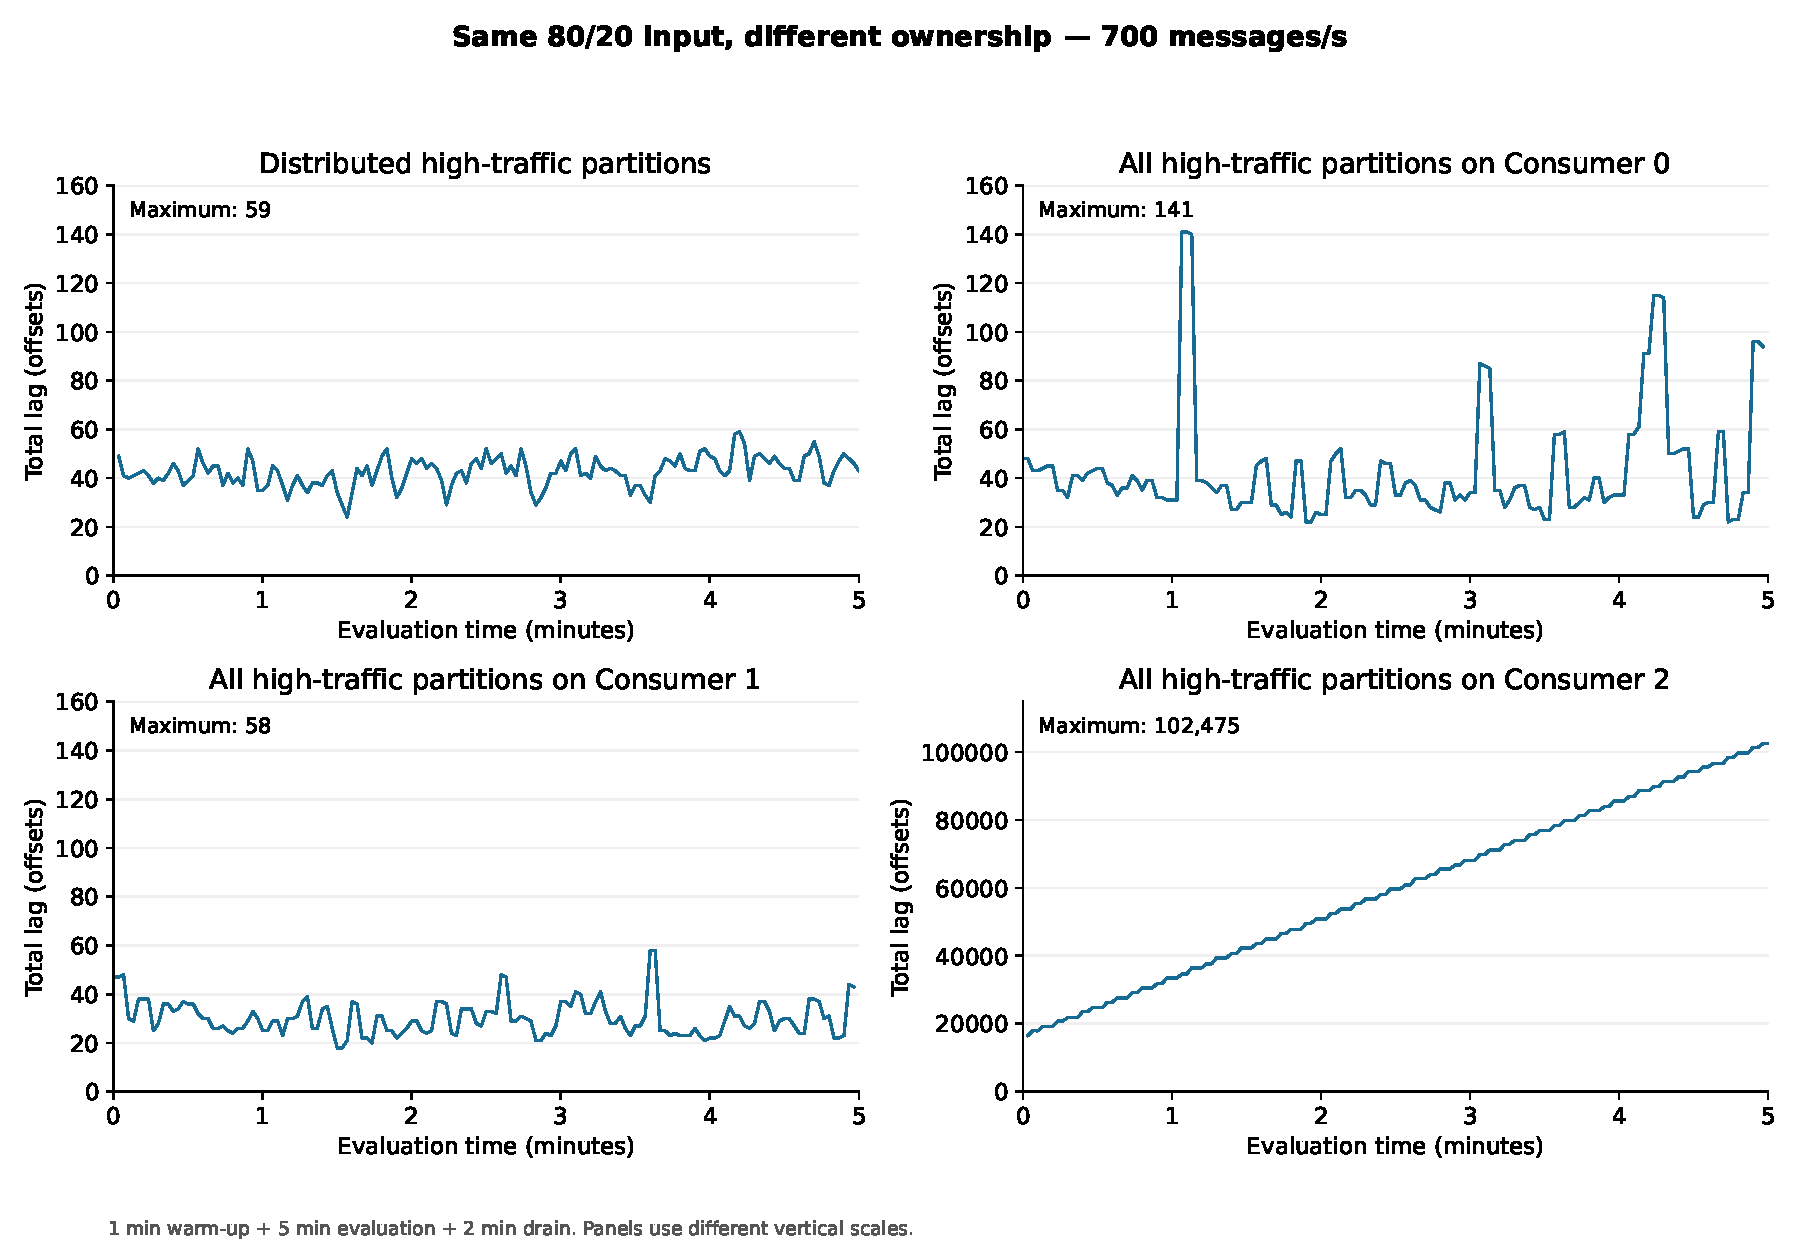
\includegraphics[width=\linewidth,height=5.40in,keepaspectratio]{figures/ownership-lag.pdf}
\caption{Total consumer-position lag during the five-minute evaluation of each fixed-ownership trial. The Consumer 2 concentration panel uses the explicitly labelled larger vertical scale. Panels show different initial layouts, not stages of a live reassignment. The full schedule also includes one minute of warm-up and two minutes of drain.}
\label{fig:ownership-total-lag}
\end{figure}
\end{landscape}

\begin{landscape}
\begin{figure}[p]
\centering
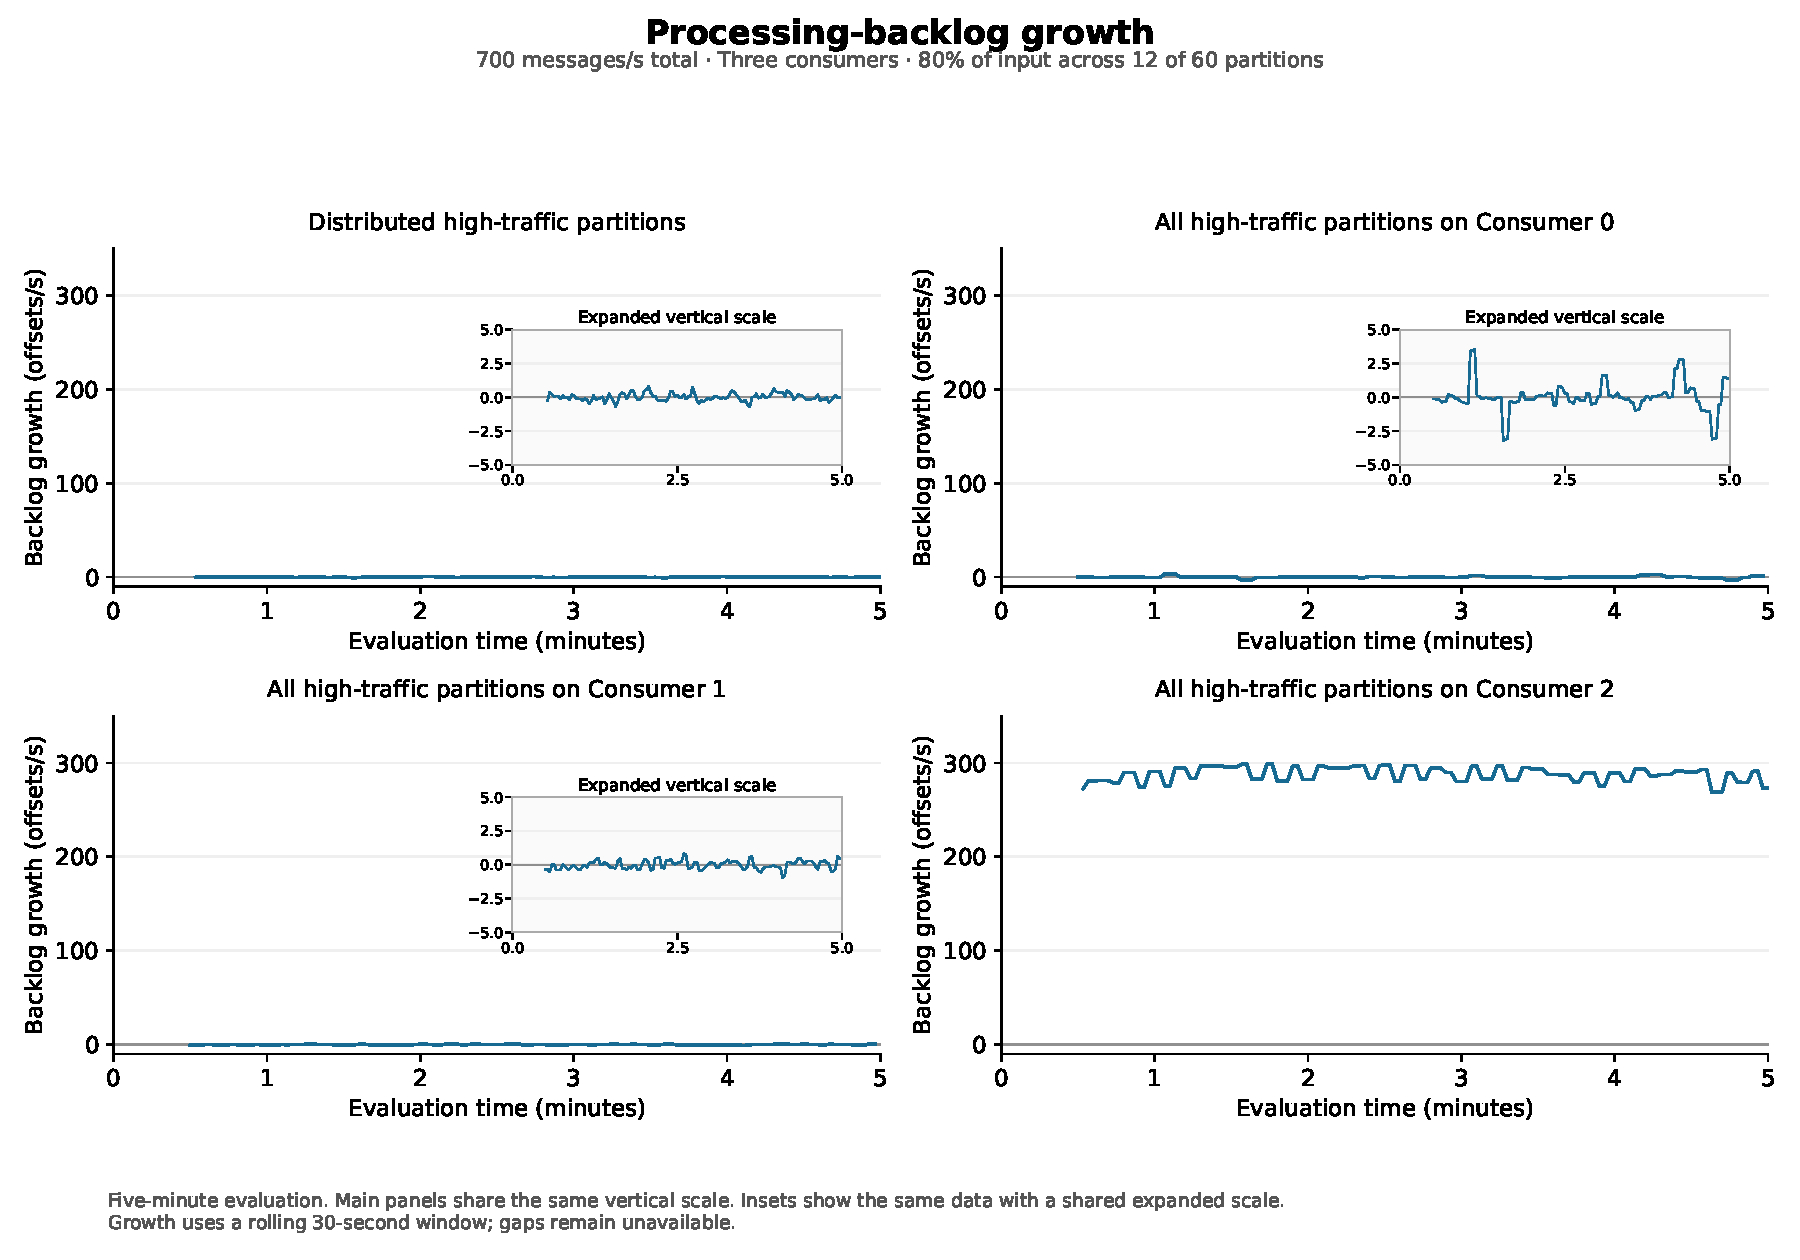
\includegraphics[width=\linewidth,height=4.90in,keepaspectratio]{figures/ownership-growth.pdf}
\caption{Rolling ten-second processing-backlog growth during evaluation. The display window was shortened from thirty seconds after the trials and applied consistently to all four layouts; complete valid windows are required after missing observations or ownership/offset resets. Main panels share a scale; labelled insets show small fluctuations. A positive growth rate indicates continued accumulation, even when the curve is approximately flat. Processing backlog is measured from the position up to which all preceding messages have completed. Consumer-position lag instead uses the position up to which the consumer has received records. The whole-evaluation summaries in Table~\ref{tab:ownership-reference-outcomes} use covered intervals without bridging monitoring gaps.}
\label{fig:ownership-backlog-growth}
\end{figure}
\end{landscape}

\begin{landscape}
\begin{figure}[p]
\centering
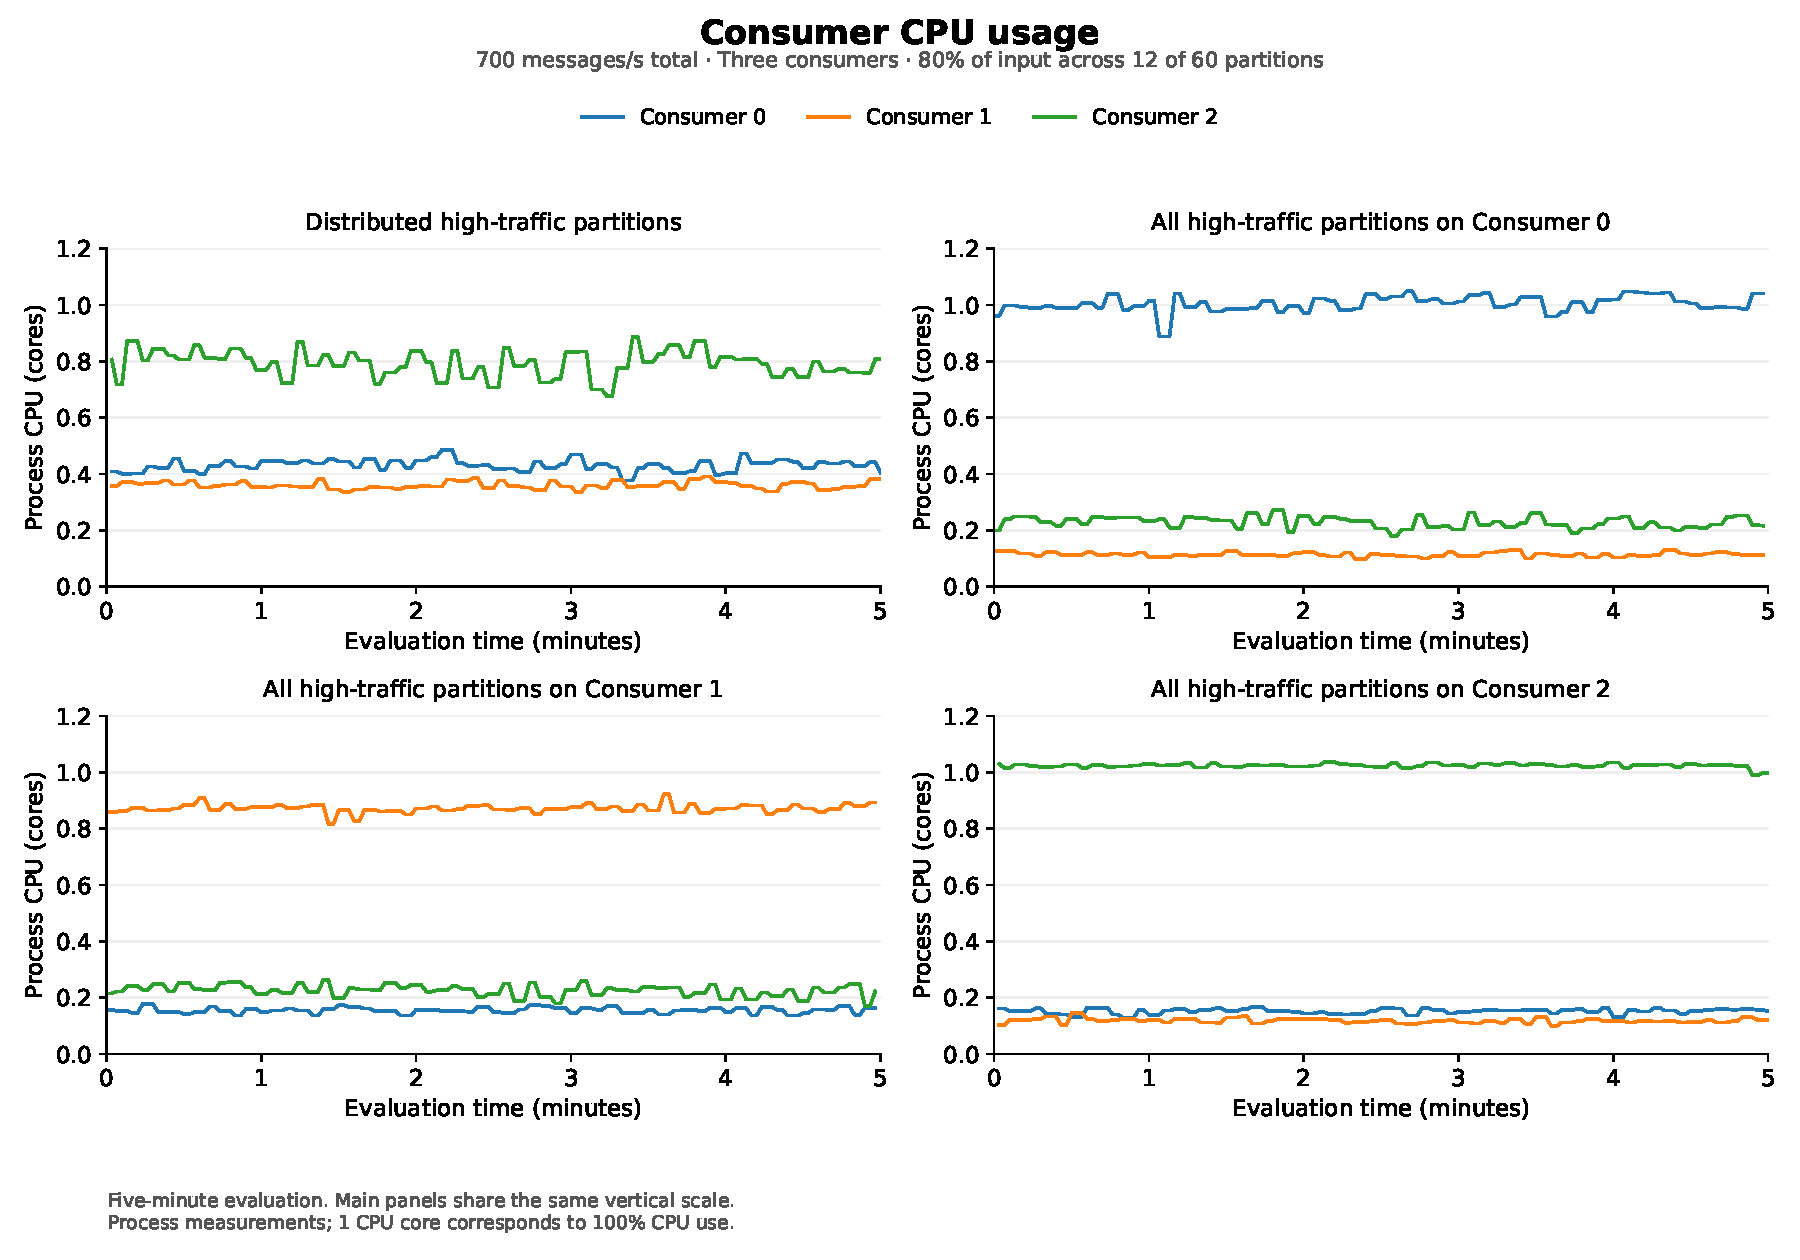
\includegraphics[width=\linewidth,height=5.40in,keepaspectratio]{figures/ownership-cpu.pdf}
\caption{Measured consumer-process CPU use during the five-minute evaluation, in cores. Panels share a scale and consistent consumer colours. These traces are process utilization, not requested CPU resources, whole-container or node utilization, or monetary charges. Shared-machine variation remains a possible influence.}
\label{fig:ownership-process-cpu}
\end{figure}
\end{landscape}

\begin{landscape}
\begin{figure}[p]
\centering
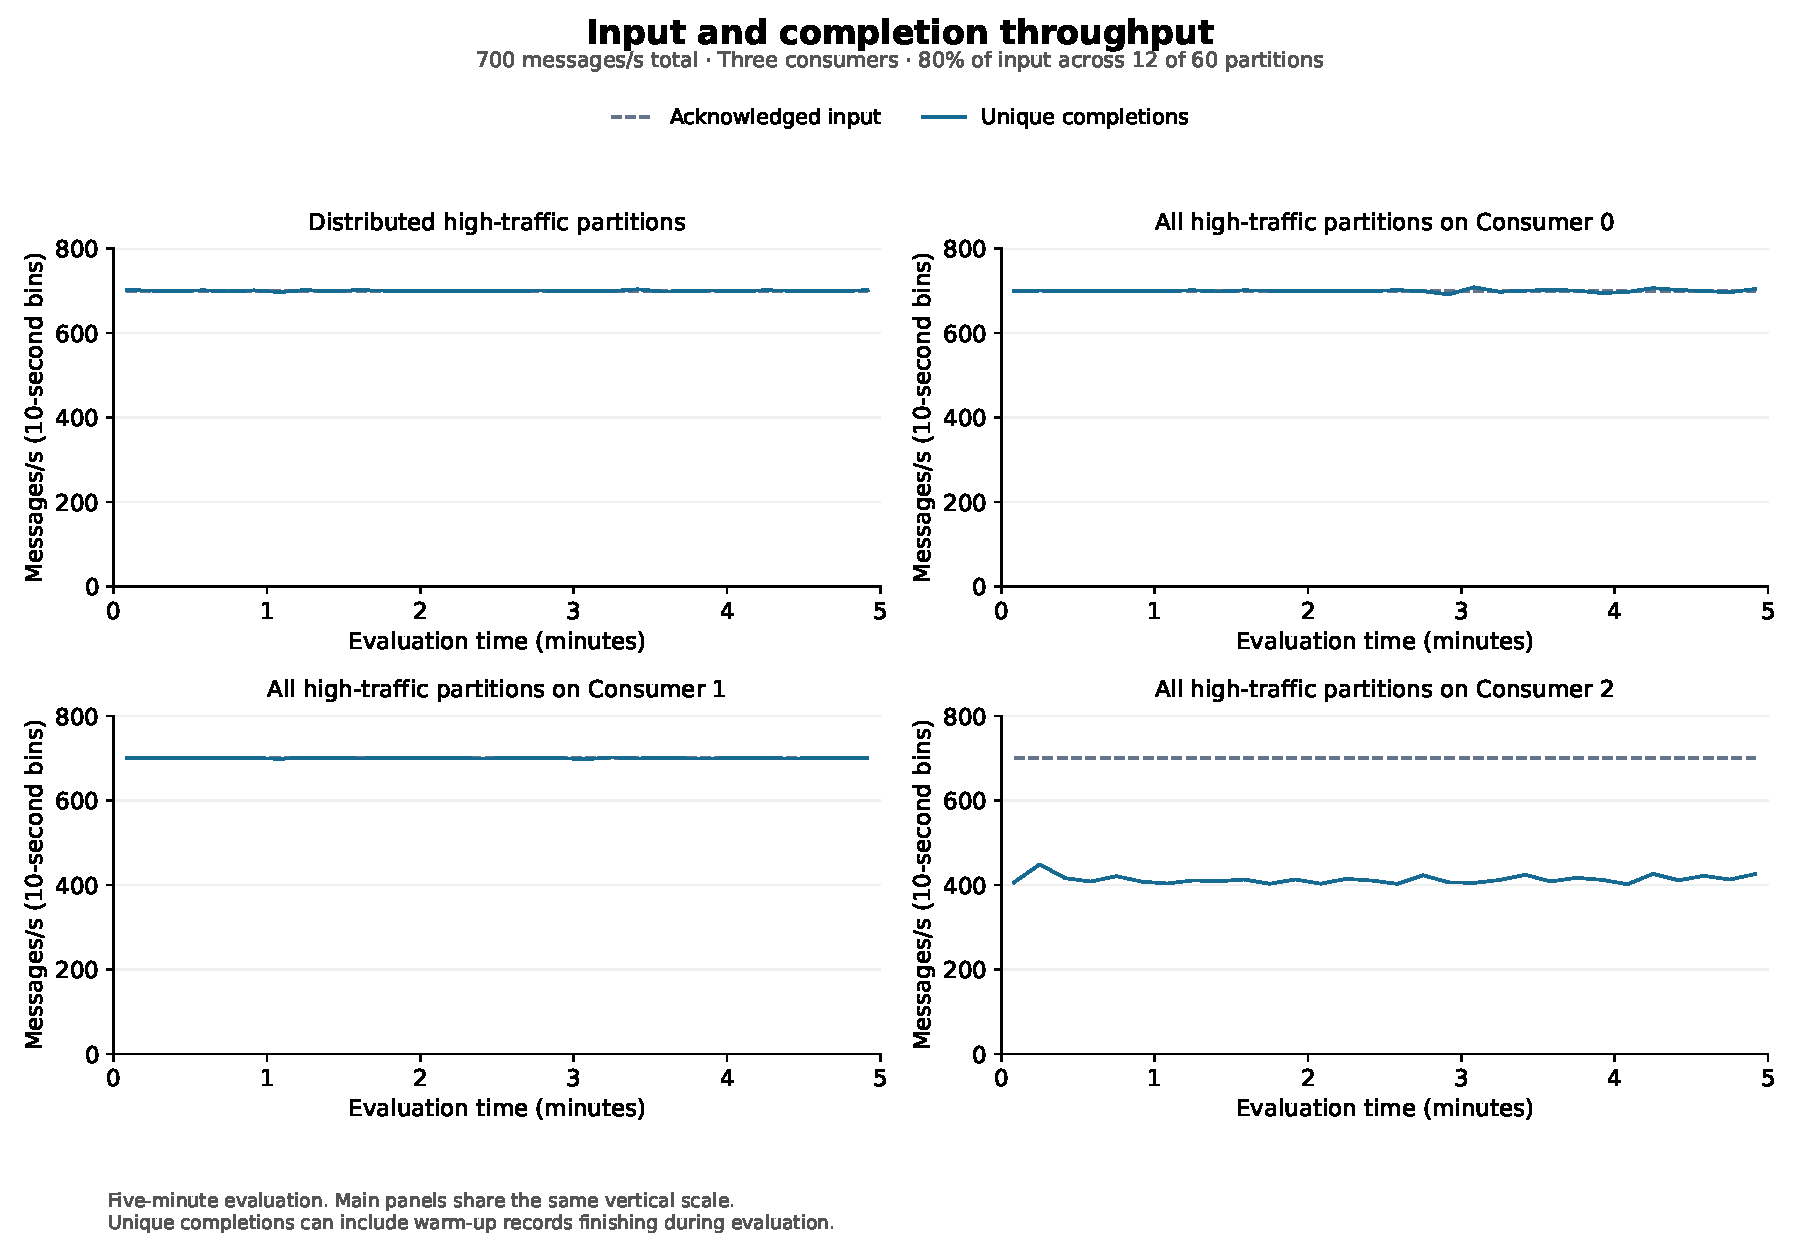
\includegraphics[width=\linewidth,height=5.40in,keepaspectratio]{figures/ownership-throughput.pdf}
\caption{Acknowledged input and distinct processing completions during evaluation. Completion throughput includes warm-up messages completed during evaluation; the latency and unfinished outcomes instead follow the messages produced during evaluation through drain. The Consumer 2 concentration trial completes fewer messages per second than arrive over the observed evaluation.}
\label{fig:ownership-throughput}
\end{figure}
\end{landscape}
\clearpage

\subsection{Live mitigation under concentrated partition ownership}
\label{sec:live-mitigation-results}

The next eight trials tested whether an observed ownership bottleneck could be relieved during processing. We retained the reference input rate of 700 messages/s, three producers, 60 partitions, and the synthetic task of 2,000 SHA-256 iterations per message. Approximately 80\% of traffic was directed to partitions 0--11. All twelve initially belonged to Consumer~2, reproducing the layout that accumulated backlog in the ownership calibration. The experiments therefore concern several busy partitions sharing one consumer, rather than a single hot key or a single indivisible overloaded partition.

Two separate four-trial blocks compared an unchanged assignment with a scheduled intervention. The first added three consumers and explicitly redistributed all 60 partitions, leaving two high-traffic and eight other partitions per consumer. The second redistributed ownership within the existing three consumers, leaving four high-traffic and sixteen other partitions per consumer. The first intervention changes both capacity and ownership; it is not a scaling-only experiment. Neither block uses an automatic decision policy or producer-side key splitting.

Each trial lasted eight minutes: one minute of warm-up, five minutes of evaluation, and two minutes of drain. In each trial, Kafka acknowledged successful publication of 210,000 messages produced during evaluation. The intervention was scheduled 60 seconds after evaluation began. Original consumer identities, nodes, resource requests and initial ownership were checked against the common reference; no additional rule forced pods onto specific nodes, and placement of added consumers remained controlled by Kubernetes. Each block used random-generation seeds 71 and 72 in the sequence unchanged Run~1, intervention Run~1, intervention Run~2, unchanged Run~2. This reverses the order of the unchanged and intervention runs across repetitions; it does not compare the execution order of different mitigation actions.

The transfers used the coordinated stop, transfer and restart procedure described in the proposal. Processing was stopped for handoff, the position up to which all preceding messages had completed and the partition owners were checked, and the new owners resumed from the recorded boundary. The observed identity, offset and handoff checks passed. These checks cover the observed handovers in the stateless synthetic trials. This experimental assignment mode is reported separately from the ordinary cooperative-sticky rebalancing evaluated in the proposal's ten-minute comparison.

\subsubsection{Adding consumers with explicit redistribution}
\label{sec:combined-results}

Adding consumers and redistributing the busy partitions reduced recorded p99 latency in both comparisons (Table~\ref{tab:live-performance}). P99 fell from 231.58 to 110.70 seconds in Run~1 and from 229.28 to 109.47 seconds in Run~2, reductions of approximately 52.2\% in both. The unchanged trials left 66,695 and 65,178 evaluation messages unfinished, whereas both intervention trials completed all evaluation messages by the drain cutoff. Figure~\ref{fig:c2-scale-outcomes} presents these two outcomes together because the baseline p99 excludes its unfinished messages.

Figure~\ref{fig:c2-scale-lag} shows backlog falling after processing resumed under the new assignment. Distinct completion throughput during evaluation increased from approximately 416--419 to 756--757 messages/s. A completion rate above the 700-message/s input rate is possible while earlier queued messages are being cleared; it is not evidence that producers exceeded their configured rate. The combined intervention demonstrates a benefit relative to retaining this concentrated assignment, but it does not establish that six consumers were necessary. Both added capacity and changed ownership contributed to the intervention being tested.

\subsubsection{Redistribution without additional consumers}
\label{sec:redistribution-results}

Redistributing the same partitions among the three existing consumers also improved the recorded outcomes. P99 fell from 226.34 to 103.76 seconds in Run~1 and from 227.13 to 91.38 seconds in Run~2, reductions of 54.2\% and 59.8\%. The unchanged trials left 63,382 and 63,998 evaluation messages unfinished, while both redistribution trials completed all evaluation messages by the cutoff. Completion throughput rose from approximately 422 to 725--728 messages/s. Figure~\ref{fig:c2-redis-outcomes} shows the completion outcomes and available lag observations.

These findings support a specific interpretation: changing whole-partition ownership can use capacity that is already available elsewhere in the consumer group. Before intervention, one consumer handled all twelve high-traffic partitions; after intervention, their processing was shared among three consumers through separate partition ownership. No partition was divided among simultaneous consumers, and no records were rerouted by key. Consequently, this result does not resolve the different case in which one partition remains overloaded even when it has a consumer to itself.

Table~\ref{tab:live-performance} reports the two separate four-trial comparisons; it does not directly rank the two interventions. P99 and unfinished percentages follow the 210,000 evaluation messages through drain. Throughput includes any warm-up messages completed during evaluation.

\begin{table}[!htbp]
\centering\small
\setlength{\tabcolsep}{3pt}
\renewcommand{\arraystretch}{1.1}
\begin{tabular}{@{}lrrrrr@{}}
\toprule
Response & Run & \shortstack{p99\\(s)} & \shortstack{Unfinished\\(\%)} & \shortstack{Misses $>1$ s\\(\%)} & \shortstack{Throughput\\(msg/s)}\\
\midrule
\multicolumn{6}{@{}l@{}}{\textbf{Scaling with targeted redistribution}}\\
Keep 3 & 1 & 231.58 & 31.760 & 83.42 & 415.93\\
Targeted scale 6 & 1 & 110.70 & 0.000 & 57.01 & 757.32\\
Keep 3 & 2 & 229.28 & 31.037 & 83.24 & 418.90\\
Targeted scale 6 & 2 & 109.47 & 0.000 & 58.17 & 755.63\\
\midrule
\multicolumn{6}{@{}l@{}}{\textbf{Redistribution within three consumers}}\\
Keep 3 & 1 & 226.34 & 30.182 & 83.41 & 422.08\\
Redistribute 3 & 1 & 103.76 & 0.000 & 61.59 & 725.25\\
Keep 3 & 2 & 227.13 & 30.475 & 83.24 & 421.76\\
Redistribute 3 & 2 & 91.38 & 0.000 & 60.84 & 727.54\\
\bottomrule
\end{tabular}
\caption{Five-minute completion outcomes and one-second SLO violations. The two blocks have separate baselines.}
\label{tab:live-performance}
\label{tab:short-targeted-scaling-outcomes}
\label{tab:short-redistribution-outcomes}
\end{table}

\clearpage
\begin{figure}[p]
\centering
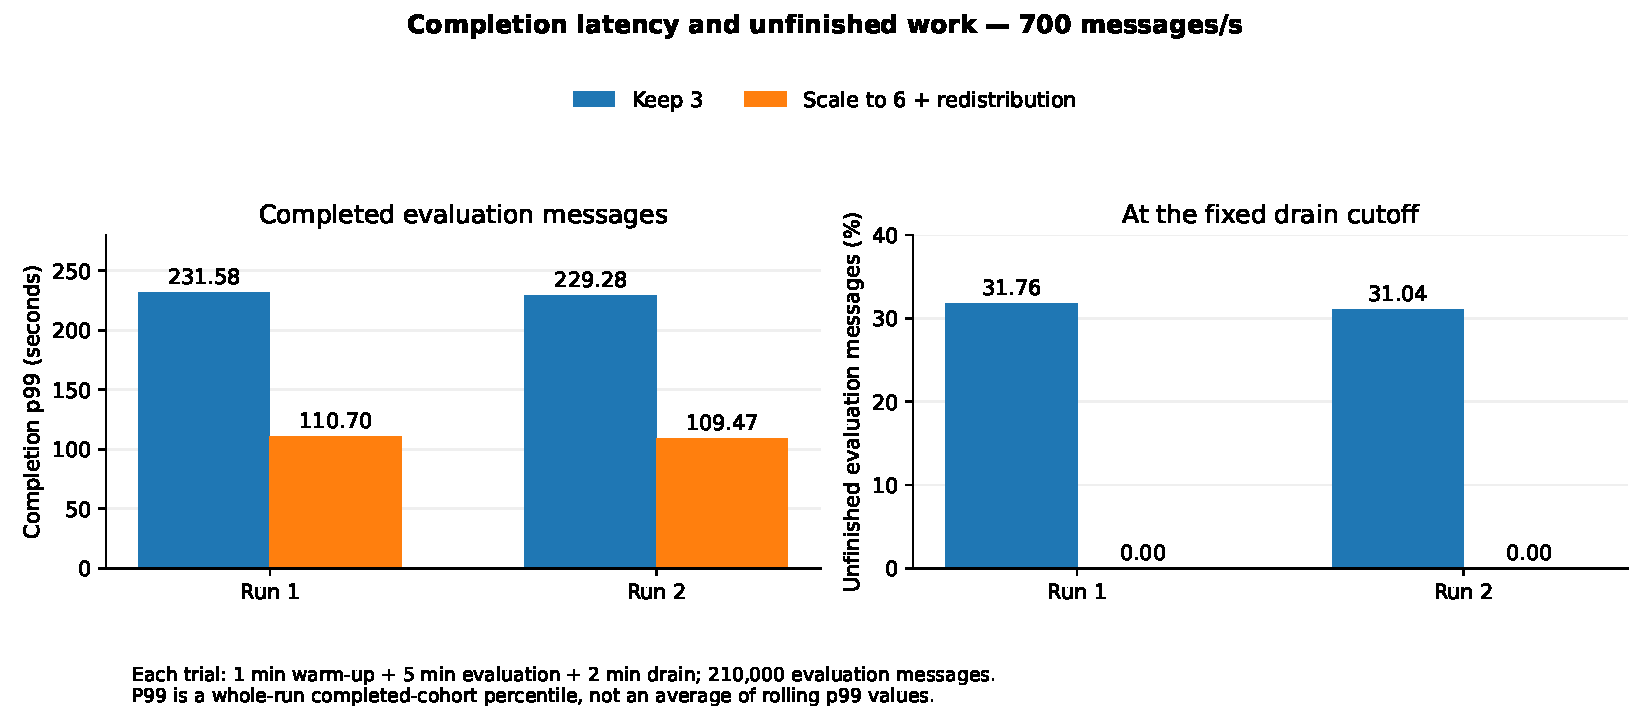
\includegraphics[width=\linewidth]{figures/c2-scaling-p99-unfinished.pdf}
\par\medskip
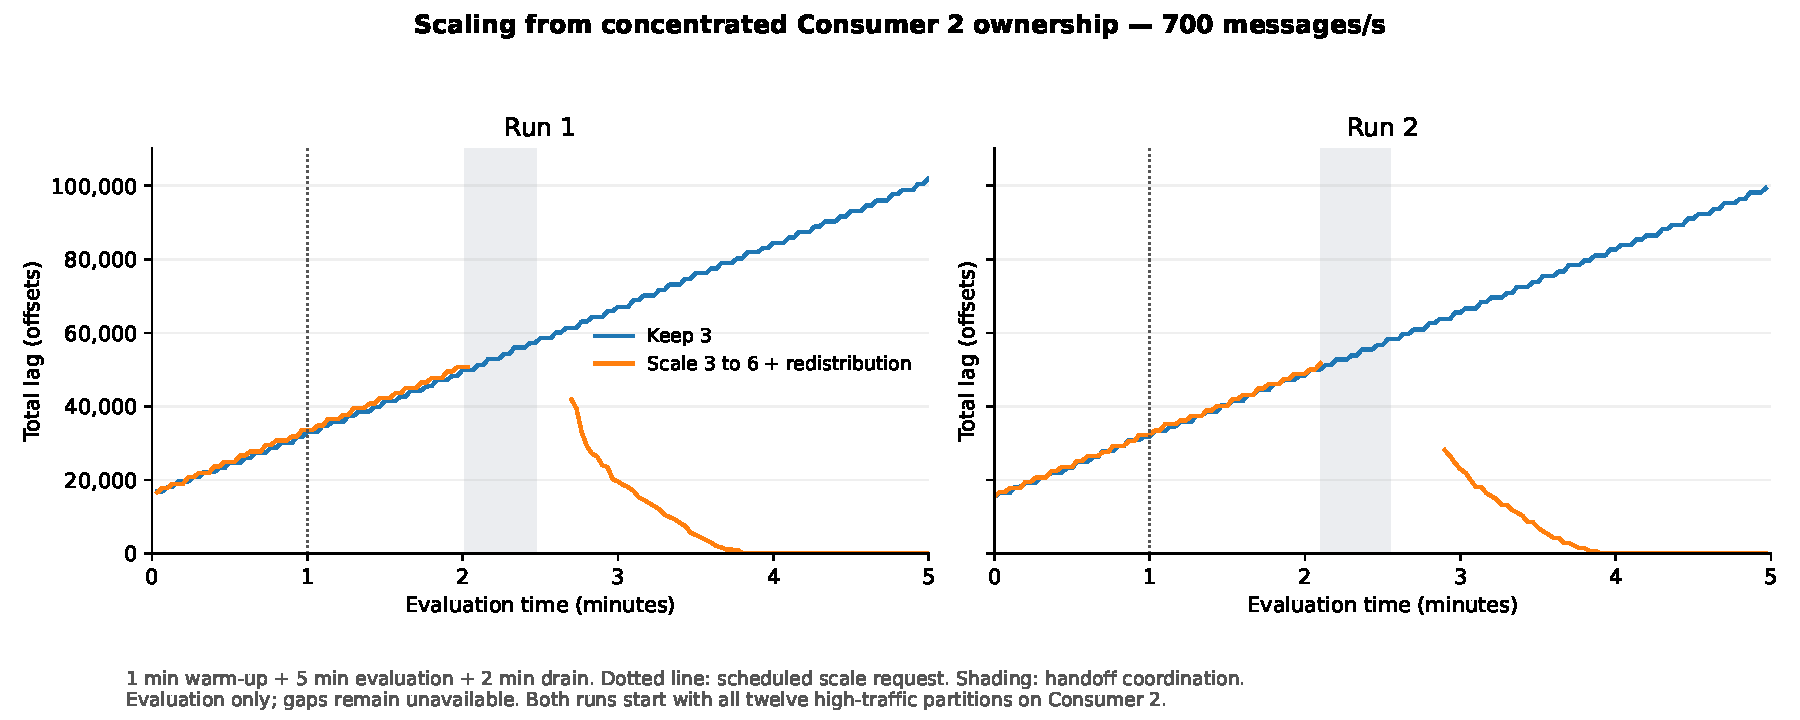
\includegraphics[width=\linewidth]{figures/c2-scaling-lag.pdf}
\caption{Scaling with targeted redistribution. Top: completed-message p99 and unfinished evaluation messages at the drain cutoff. Bottom: consumer-position lag during evaluation. Baseline coverage is 99.3\%; intervention coverage is 86.0\% and 83.3\%. Gaps remain unavailable observations.}
\label{fig:c2-scale-outcomes}
\label{fig:c2-scale-lag}
\end{figure}
\clearpage
\begin{figure}[p]
\centering
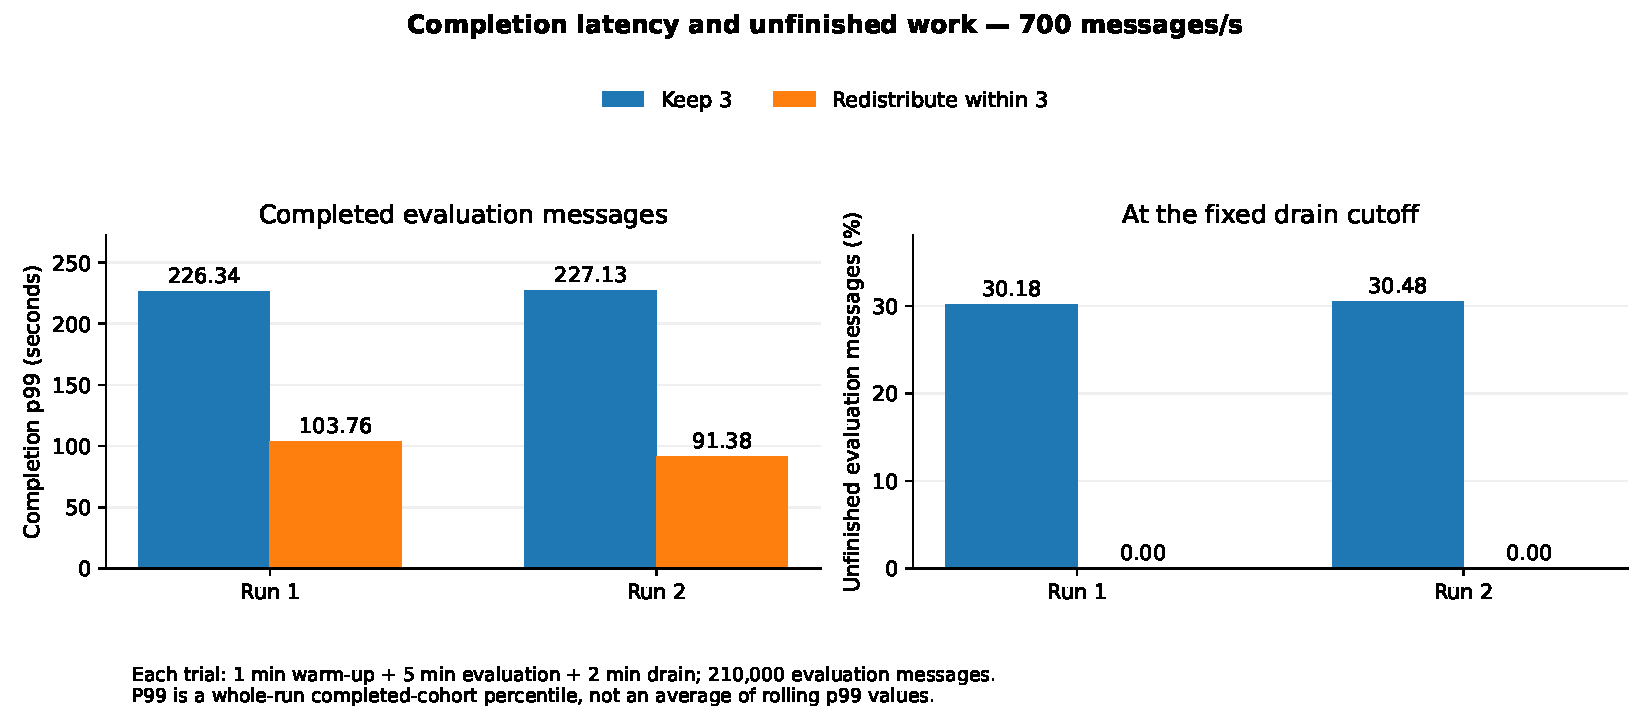
\includegraphics[width=\linewidth]{figures/c2-redistribution-p99-unfinished.pdf}
\par\medskip
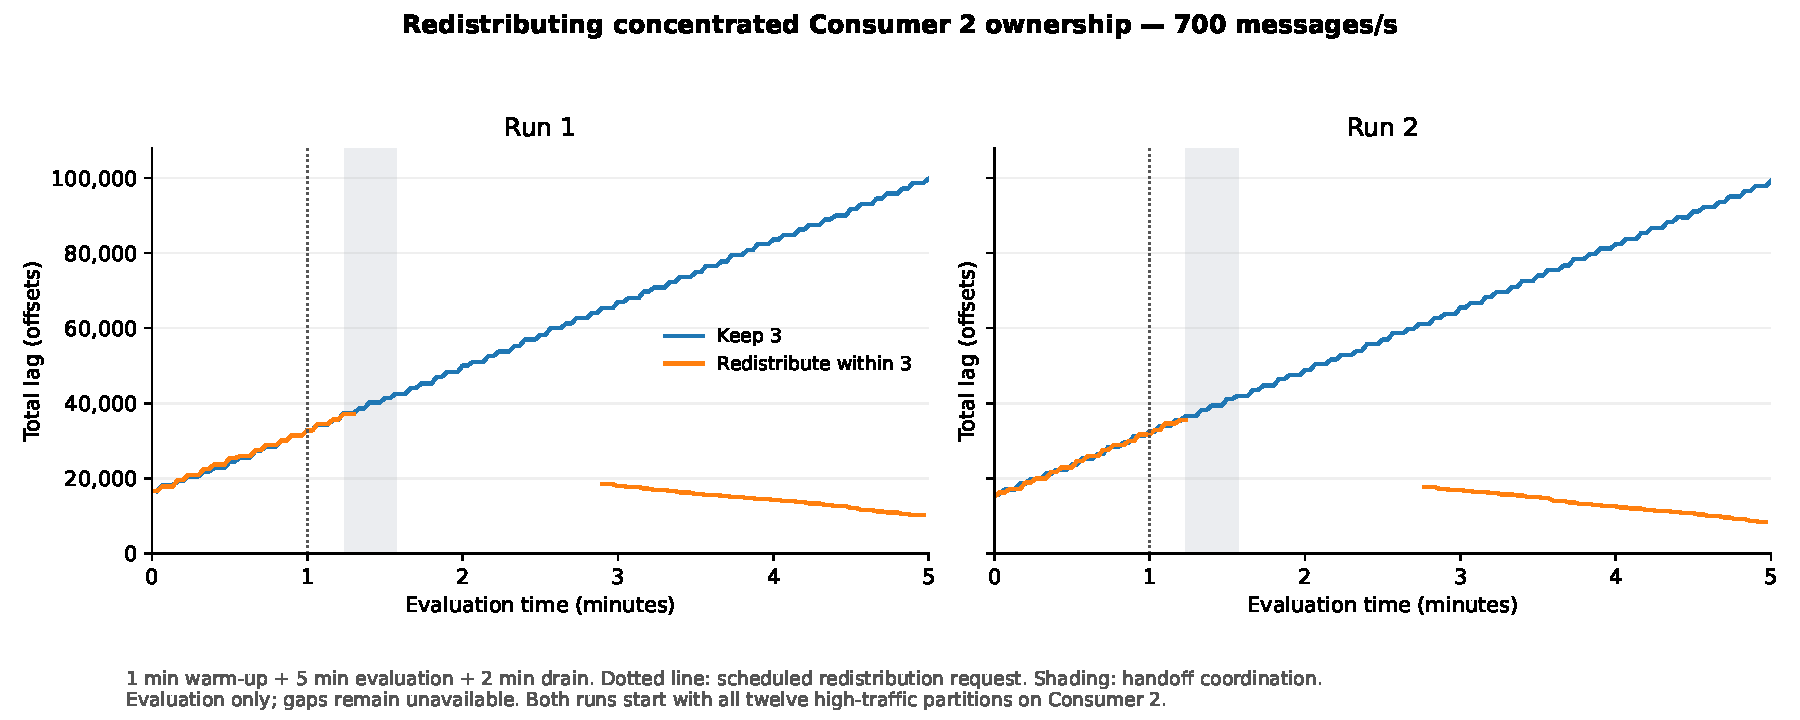
\includegraphics[width=\linewidth]{figures/c2-redistribution-lag.pdf}
\caption{Redistribution within three consumers. Top: completed-message p99 and unfinished evaluation messages at the drain cutoff. Bottom: consumer-position lag during evaluation. Intervention coverage is 67.3\% and 68.7\%, versus 99.3\% in the baselines. These gaps do not represent an equally long processing pause.}
\label{fig:c2-redis-outcomes}
\label{fig:c2-redis-lag}
\end{figure}
\clearpage

\subsection{Resource requirements, interruption and recovery}
\label{sec:live-cost-results}

Redistribution improved completion outcomes without increasing requested consumer resources. All four trials in that block used 42.00 core-minutes of requested CPU and 21.00 GiB-minutes of requested memory over the seven-minute evaluation-plus-drain interval, with complete allocation-history coverage. In contrast, the combined interventions requested approximately 76.70 and 76.81 core-minutes and 38.35 and 38.40 GiB-minutes. Table~\ref{tab:live-resources} keeps CPU and memory separate and identifies the incomplete resource record in the second combined baseline. These quantities measure requested resources over time, not cloud charges.

Unchanged requests do not imply unchanged resource use. In the redistribution block, observed consumer-process CPU increased from 515.77 to 554.06 core-seconds in Run~1 and from 516.49 to 553.41 core-seconds in Run~2 while more messages completed. The corresponding resident memory accumulated over time changed from 93.71 to 88.36 and from 93.07 to 87.44 GiB-seconds. These process integrals cover approximately 99.52\% of evaluation plus drain and exclude unobserved intervals. They describe consumer-process activity and memory footprint, not whole-cluster consumption. CPU, memory, throughput, growth and lag-skew traces are retained in Section~\ref{app:live-diagnostics}.

Table~\ref{tab:live-resources} covers five minutes of evaluation and two minutes of drain; warm-up is excluded from resource totals. The starred second baseline for scaling with redistribution has only partial resource-history coverage and cannot support a complete-period cost ratio. Missing resource history does not mean zero allocation.

\begin{table}[!htbp]
\centering\small
\setlength{\tabcolsep}{3pt}
\renewcommand{\arraystretch}{1.1}
\begin{tabular}{@{}lrrrrr@{}}
\toprule
Response & Run & \shortstack{Actual CPU\\(core-s)} & \shortstack{Actual RSS\\(GiB-min)} & \shortstack{Requested CPU\\(core-min)} & \shortstack{Requested memory\\(GiB-min)}\\
\midrule
\multicolumn{6}{@{}l@{}}{\textbf{Scaling with targeted redistribution}}\\
Keep 3 & 1 & 515.3 & 1.57 & 42.00 & 21.00\\
Targeted scale 6 & 1 & 704.8 & 2.27 & 76.70 & 38.35\\
Keep 3 & 2 & 519.5 & 1.56 & 33.75$^{*}$ & 16.87$^{*}$\\
Targeted scale 6 & 2 & 687.6 & 2.25 & 76.81 & 38.40\\
\midrule
\multicolumn{6}{@{}l@{}}{\textbf{Redistribution within three consumers}}\\
Keep 3 & 1 & 515.8 & 1.56 & 42.00 & 21.00\\
Redistribute 3 & 1 & 554.1 & 1.47 & 42.00 & 21.00\\
Keep 3 & 2 & 516.5 & 1.55 & 42.00 & 21.00\\
Redistribute 3 & 2 & 553.4 & 1.46 & 42.00 & 21.00\\
\bottomrule
\end{tabular}
\caption{Consumer resources over five minutes of evaluation and two minutes of drain. Warm-up is excluded.}
\label{tab:live-resources}
\label{tab:short-targeted-scaling-resources}
\label{tab:short-redistribution-resources}
\par\smallskip\begin{minipage}{\linewidth}\footnotesize $^{*}$Only 80.36\% of the requested-resource history was available for this baseline; these partial totals cannot support a full-period cost ratio. The other request histories cover 100\%. Actual CPU and RSS totals use observed intervals. RSS is resident set size, the memory held by a consumer process.\end{minipage}
\end{table}

\clearpage
\subsubsection{Processing interruption and continuing-input recovery}
Both interventions temporarily interrupted processing. The combined-action trials had observed processing gaps of 20.20 and 19.99 seconds; redistribution within three consumers had gaps of 15.29 and 15.26 seconds (Table~\ref{tab:live-transition}). These gaps were checked against recorded processing intervals and handoff events. They are not the same as pod startup time, an ordinary Kafka rebalance duration, or the full interval between the scheduled action and verification of the new assignment. Approximate cross-host timing remains subject to the recorded clock-probe uncertainty.

Messages continued to arrive during these interruptions. The event records show increases of 14,143 and 13,992 acknowledged but unfinished messages during the combined-action gaps, and 10,700 and 10,682 during the redistribution-only gaps. Figure~\ref{fig:c2-scale-events} reconstructs unfinished work from message identifiers and acknowledgment and completion times, including warm-up messages. This provides evidence during invalid offset-monitoring intervals. It is a different measurement from consumer-position lag and does not by itself show how many additional unfinished messages the intervention caused compared with running without an intervention.

In Table~\ref{tab:live-transition}, active ownership means that the new assignment has been verified. Processing may resume before this check finishes, so the reported intervals have different endpoints and are not interchangeable.

\begin{table}[!htbp]
\centering\small
\setlength{\tabcolsep}{3pt}
\begin{tabular}{@{}lrrrr@{}}
\toprule
\textbf{Intervention} & \textbf{Processing} & \textbf{Release to} & \textbf{Scheduled to} & \textbf{Unfinished increase}\\
 & \textbf{gap (s)} & \textbf{active (s)} & \textbf{active (s)} & \textbf{during gap}\\
\midrule
Combined, Run 1 & 20.20 & 27.03 & 88.28 & 14,143\\
Combined, Run 2 & 19.99 & 26.55 & 92.79 & 13,992\\
Redistribution, Run 1 & 15.29 & 19.29 & 34.26 & 10,700\\
Redistribution, Run 2 & 15.26 & 19.38 & 33.78 & 10,682\\
\bottomrule
\end{tabular}
\caption{Handover times and additional unfinished work.}
\label{tab:live-transition}
\end{table}

Recovery while input continues is a stricter outcome than completing all evaluation messages after producers stop. For these blocks, the diagnostic requires total processing backlog to remain at or below 100 offsets for 30 consecutive seconds, with valid observations from the same partition owners and no gaps exceeding three seconds. In the combined block, recovery was confirmed approximately 120.4 and 117.7 seconds after resume. That recovery check was defined after the combined-action trials. The same criterion was fixed before the redistribution-only block, where neither trial confirmed recovery before production ended; thresholds of 50 and 200 offsets gave the same unconfirmed result.

The redistribution trials were nevertheless catching up near the end of evaluation. Over the final two minutes, covered processing-backlog growth was approximately $-65.7$ and $-72.9$ offsets/s, but the last valid backlogs were still 10,166 and 8,326 offsets. The subsequent drain allowed all evaluation messages to finish. Thus, the observations support improved processing and less unfinished work at the cutoff, while leaving open whether the unchanged input could be sustained with a sufficiently small backlog over a longer period.

\clearpage
\begin{figure}[p]
\centering
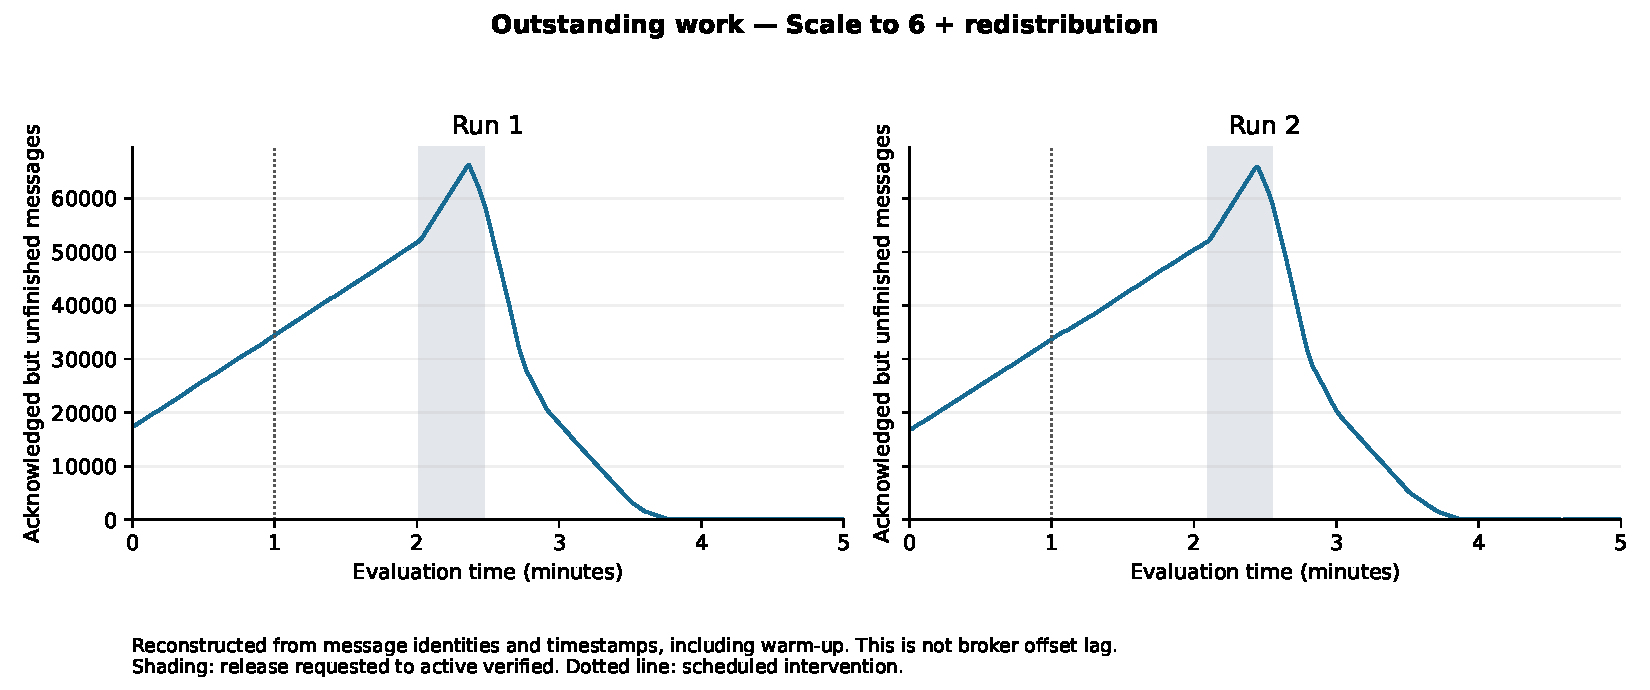
\includegraphics[width=\linewidth]{figures/c2-scaling-intervention-cost-backlog.pdf}
\par\medskip
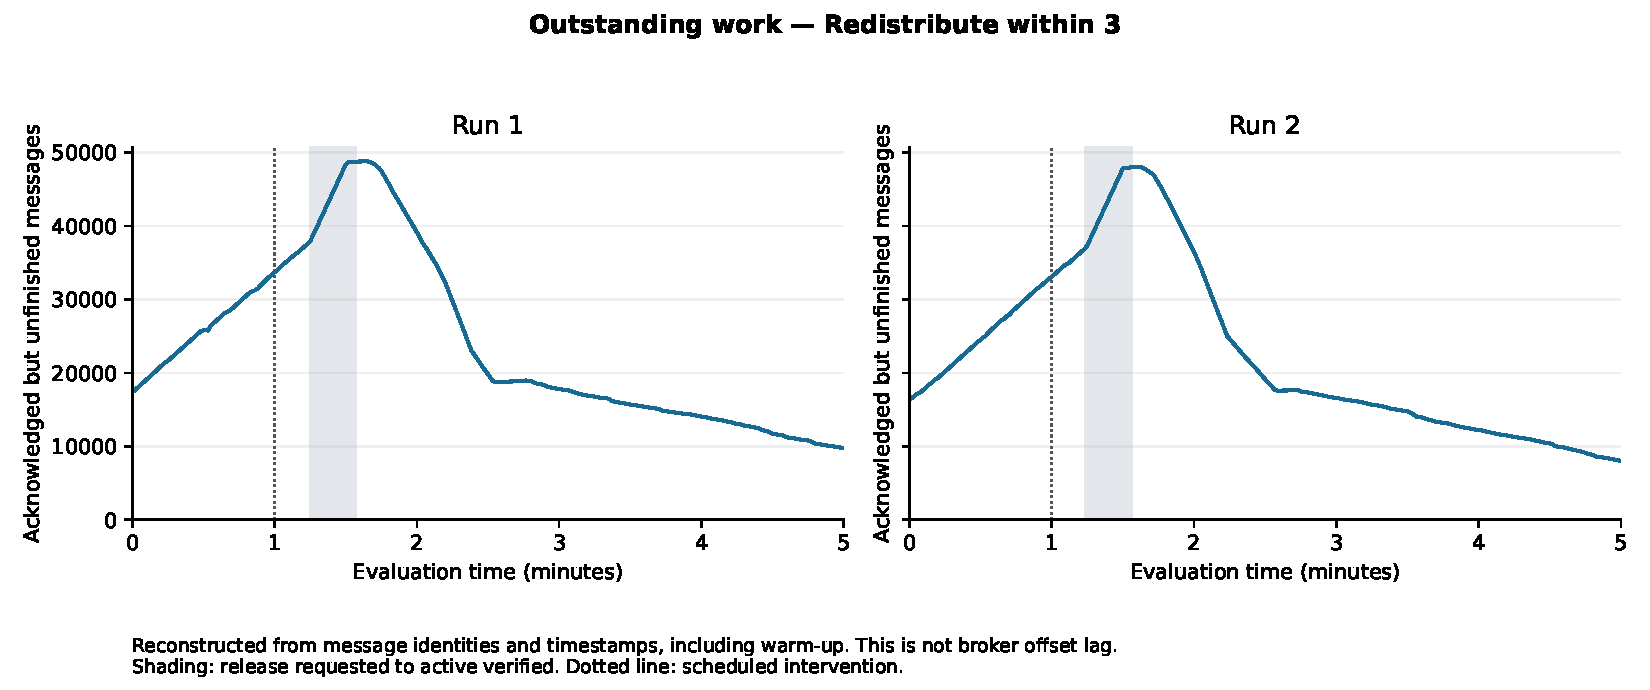
\includegraphics[width=\linewidth]{figures/c2-redistribution-intervention-cost-backlog.pdf}
\caption{Acknowledged but unfinished messages around the intervention. Top: scaling with targeted redistribution. Bottom: redistribution within three consumers. Counts are reconstructed from message events and include warm-up work. They are distinct from offset-based lag and evaluation-only unfinished messages at drain.}
\label{fig:c2-scale-events}
\label{fig:c2-redis-events}
\end{figure}
\clearpage



\clearpage
\section{Supporting Ownership Diagnostics}
\label{app:ownership-diagnostics}

Figures~\ref{fig:ownership-process-memory}--\ref{fig:ownership-consumer-lag} complete the seven metric comparisons for the four 700-message/s ownership trials. All show only the five-minute evaluation interval, with distributed ownership and concentration on Consumers 0, 1 and 2 in the same display order. Each full trial includes one minute of warm-up and two minutes of drain. Display order is different from the actual execution order (distributed, C0, C2, C1).

Consumer 2's mean resident memory, the physical memory occupied by its process, reached 145.4\,MiB in its concentrated trial, compared with approximately 31.9\,MiB for the other consumers in that trial. The cause of this process-memory difference was not identified. The measurement does not represent all memory used on the node. The mean lag-skew ratios across valid observations were 9.241, 9.252, 10.004 and 4.927 in display order. These are means of valid maximum/mean partition-lag ratios, not ratios derived from aggregate lag means. The lower ratio in the overloaded case illustrates the need to interpret relative skew together with backlog magnitude and growth.

\begin{landscape}
\begin{figure}[p]
\centering
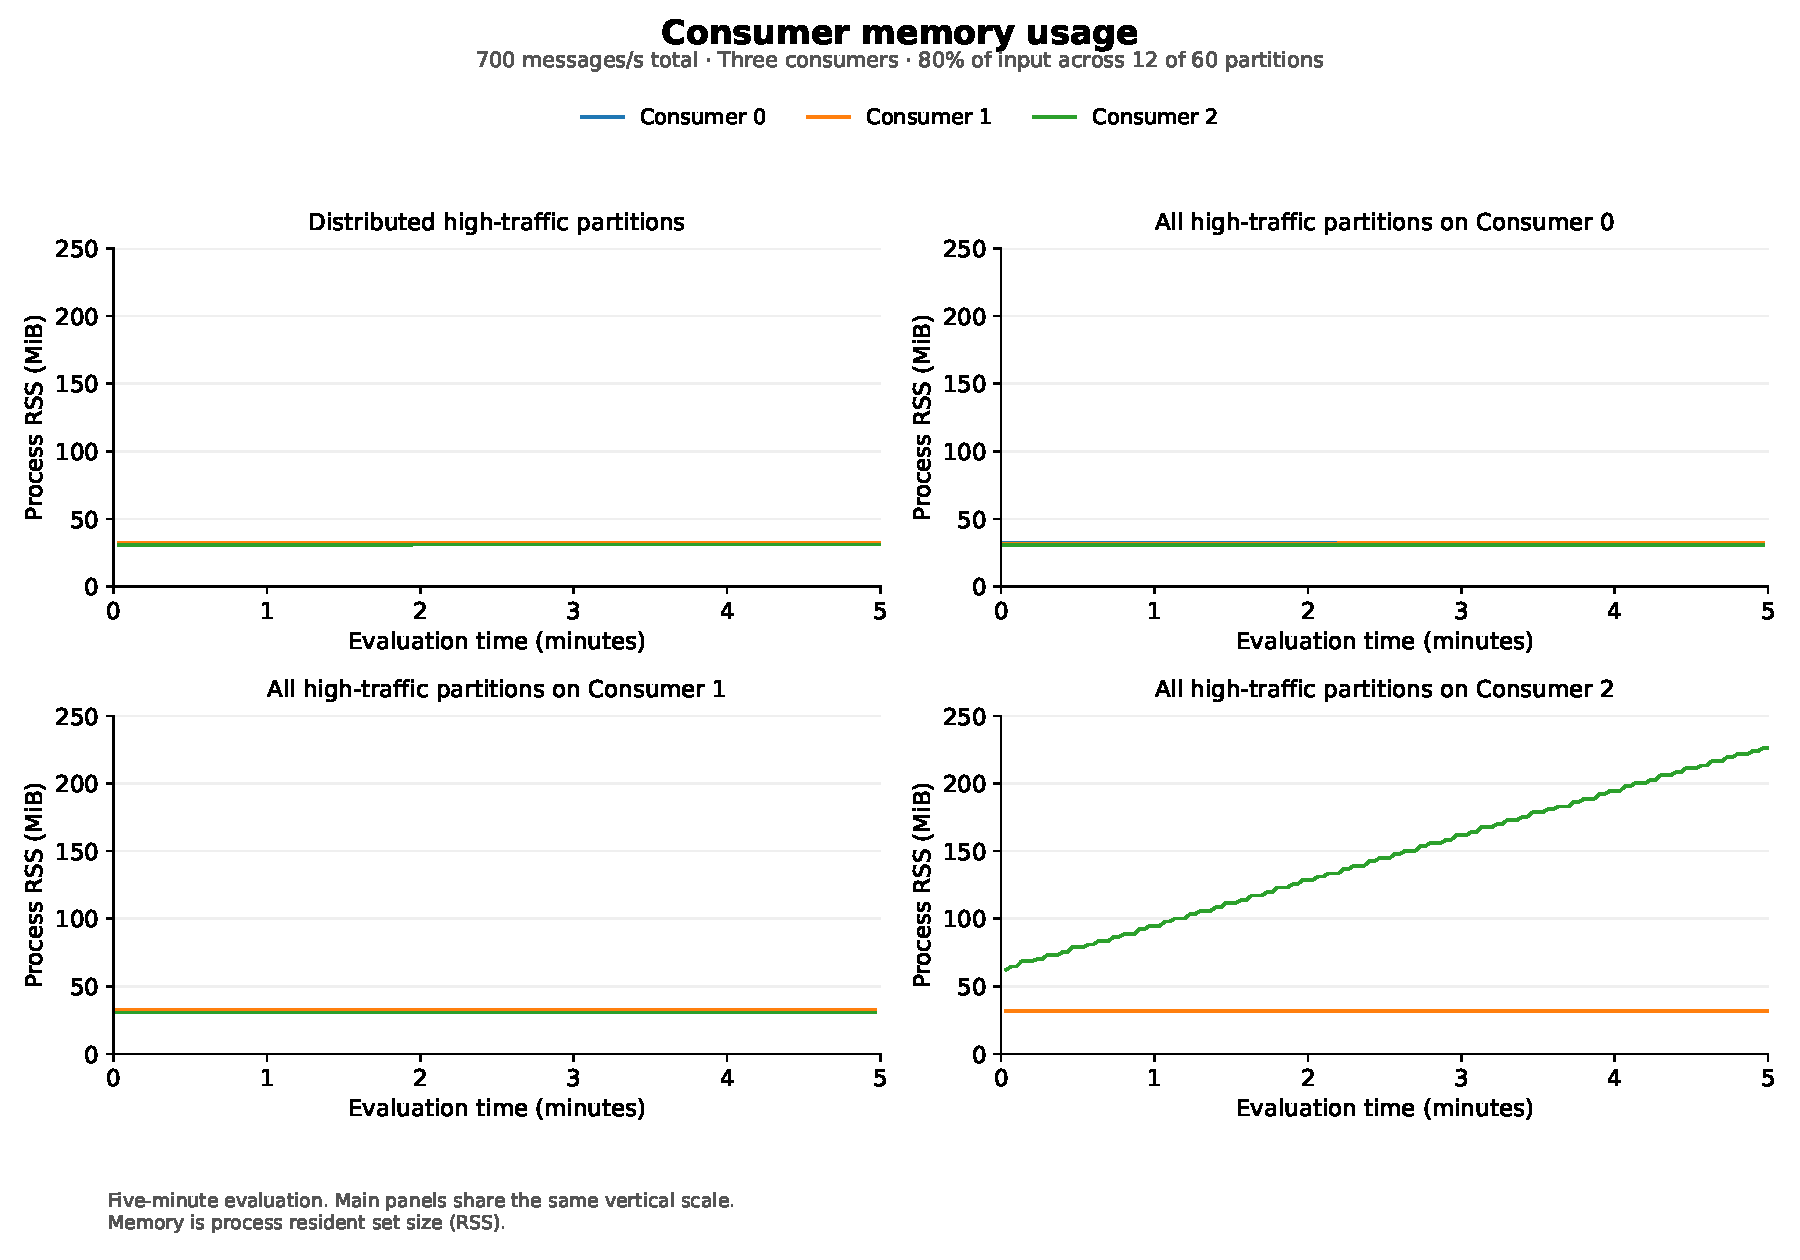
\includegraphics[width=\linewidth,height=5.40in,keepaspectratio]{figures/ownership-memory.pdf}
\caption{Consumer-process resident memory (RSS) during evaluation. Panels share a scale. The concentrated Consumer 2 trial shows increased process memory, but the source of the allocation is not isolated. These measurements exclude other processes, brokers and node-wide memory use.}
\label{fig:ownership-process-memory}
\end{figure}
\end{landscape}

\begin{landscape}
\begin{figure}[p]
\centering
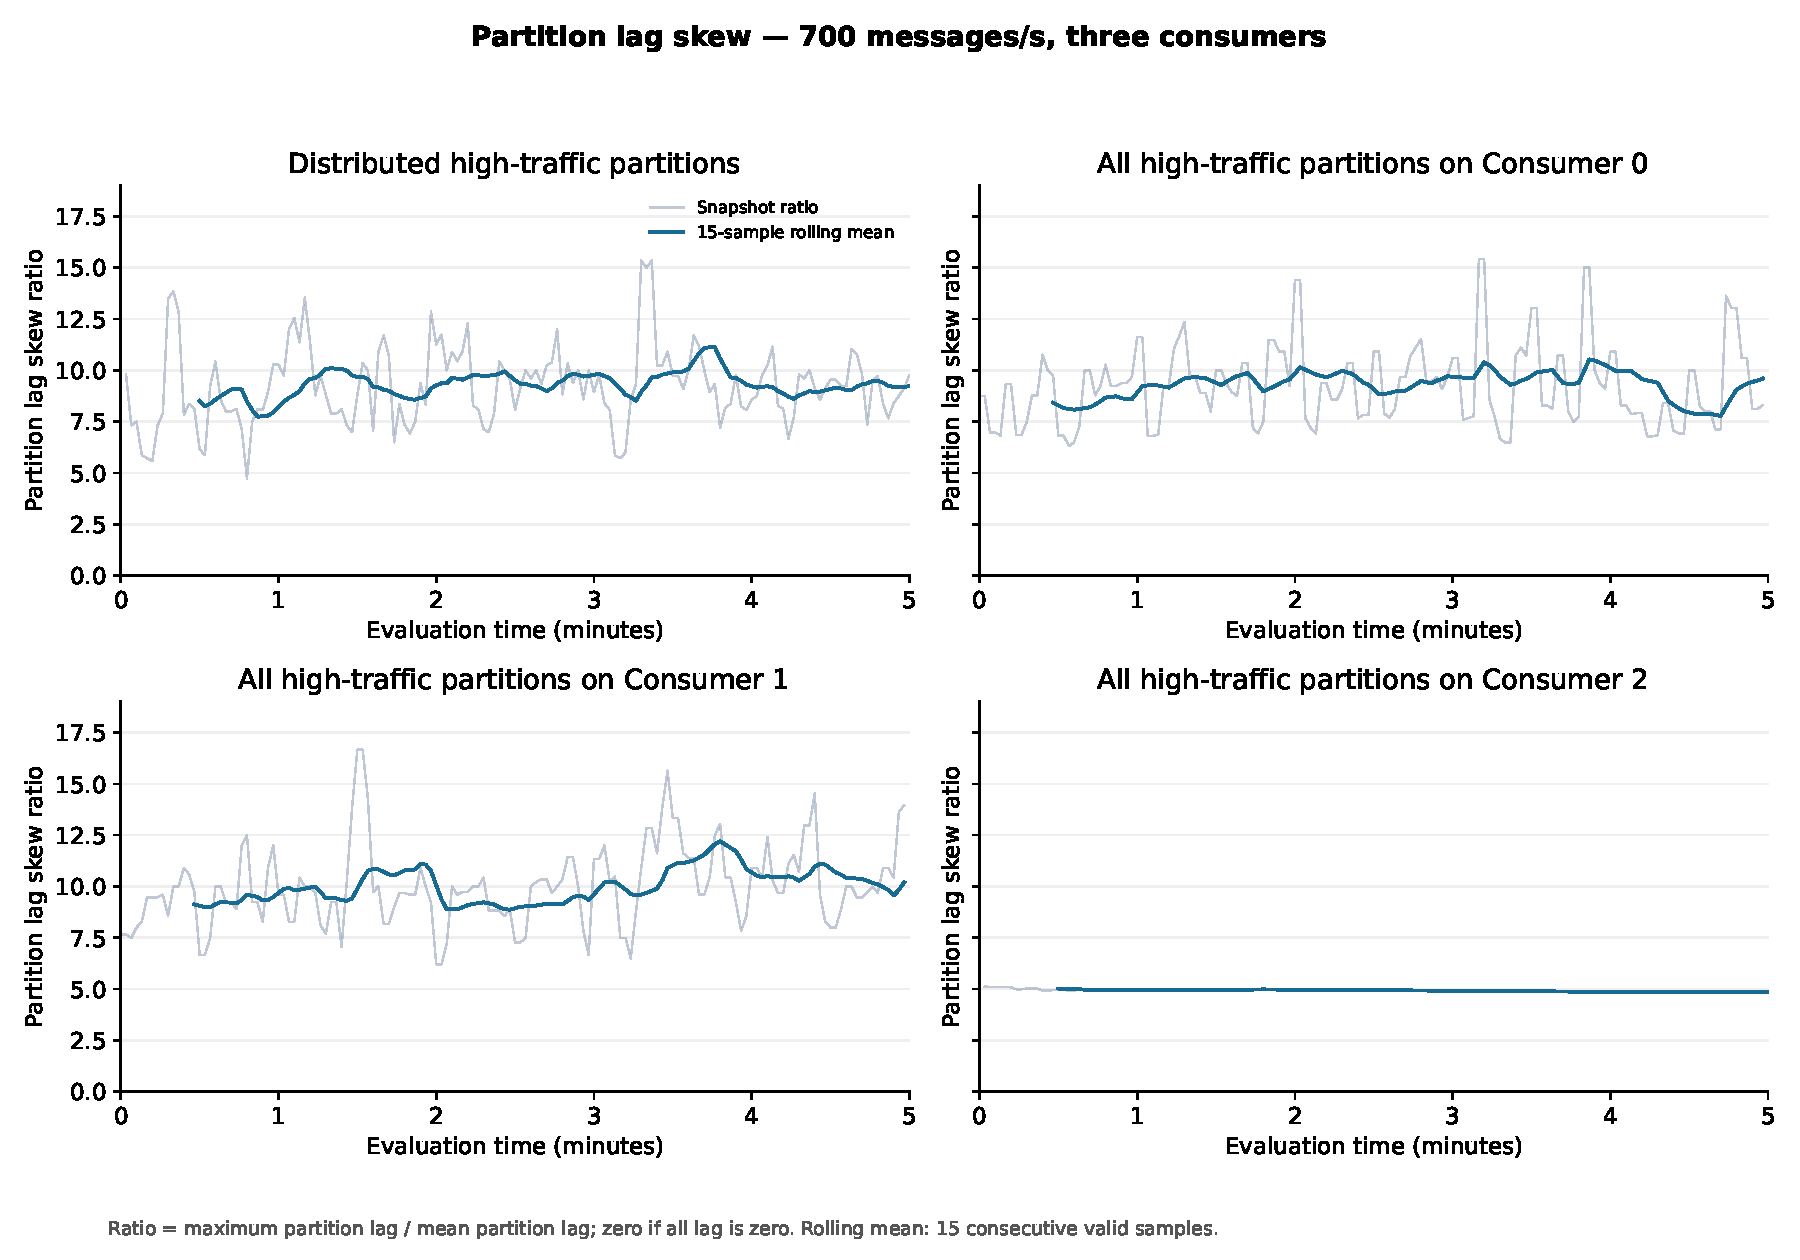
\includegraphics[width=\linewidth,height=5.40in,keepaspectratio]{figures/ownership-skew.pdf}
\caption{Partition lag-skew ratio, defined as maximum partition lag divided by mean partition lag. A high ratio can occur when absolute lag is small. The Consumer 2 concentration trial has substantial lag across multiple high-traffic partitions and a lower mean ratio than the low-lag layouts.}
\label{fig:ownership-skew}
\end{figure}
\end{landscape}

\begin{landscape}
\begin{figure}[p]
\centering
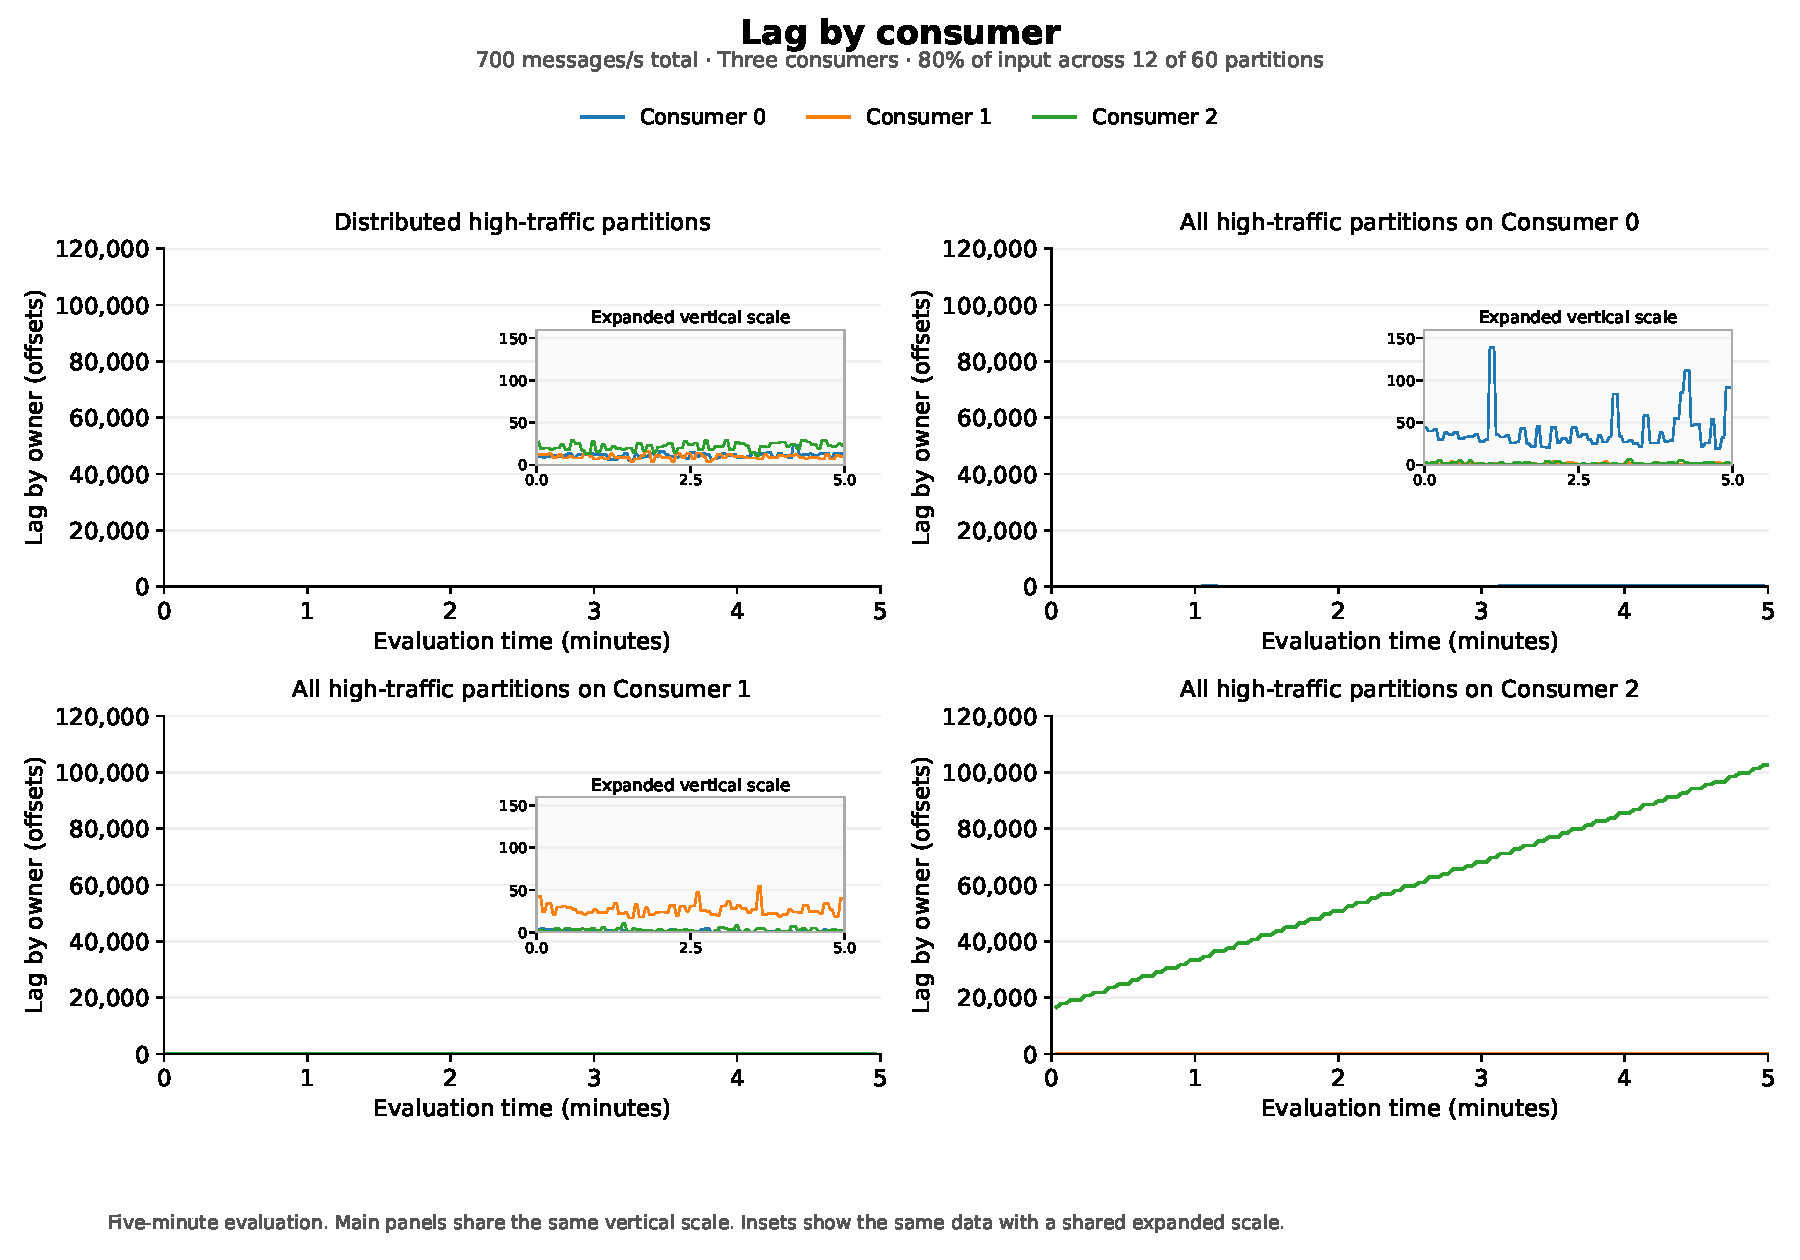
\includegraphics[width=\linewidth,height=5.40in,keepaspectratio]{figures/ownership-owners.pdf}
\caption{Consumer-position lag grouped by the fixed partition owner. Main panels share a scale, while labelled insets expand the small fluctuations. The large lag in the Consumer 2 concentration trial is associated with its assigned partitions. These are fixed initial assignments, not before/after observations of live redistribution.}
\label{fig:ownership-consumer-lag}
\end{figure}
\end{landscape}

\clearpage

\begingroup
\emergencystretch=3em
\clearpage
\section{Supporting Measurements for Live Interventions}
\label{app:live-diagnostics}

The first set of figures retains the per-consumer and time-dependent measurements for the two earlier live-intervention blocks. Each figure compares separate eight-minute trials, comprising one minute of warm-up, five minutes of evaluation and two minutes of drain. The plotted interval is the five-minute evaluation unless stated otherwise. Request markers and shaded coordination intervals describe recorded intervention events; blank intervals remain unavailable observations.

\subsection{Monitoring coverage and interpretation}
Table~\ref{tab:live-lag-coverage} reports consumer-position lag only over valid monitoring intervals. The baseline series cover approximately 99.3\% of evaluation, whereas the intervention series lose coverage around ownership transfer. In particular, the redistribution trials contain intervals without valid lag measurements of approximately evaluation seconds 80--172 and 76--164. Their duration does not equal the approximately 15.3-second verified processing interruption. Neither the sampled maximum nor the mean establishes the true full-transition backlog when observations are missing. The event-derived outstanding-work figures in Section~\ref{sec:live-cost-results} provide complementary evidence without filling these gaps.

AWS documents a related monitoring limitation in Amazon MSK: consumer-lag metrics are emitted only for groups in the \texttt{STABLE} or \texttt{EMPTY} states and are absent while a group is unstable~\cite{awsMskConsumerLag}. This concerns missing measurements, not lost records, and does not establish the cause of gaps in this pipeline.

% Earlier wording retained for reference.
% These five-minute intervention trials used an earlier monitoring implementation. A subsequent technical validation identified why lag remained unavailable after processing resumed: the client position was unresolved until each newly assigned partition first returned a record, despite a verified starting offset for the new assignment. The corrected monitor uses that start only before the partition returns any record and while its client position remains unresolved. The monitor still requires current broker offset limits, valid recorded offsets, and exactly one assigned consumer for each partition. The monitor stops using the temporary starting position once the partition returns records or its ownership is released or revoked. Genuine handover intervals remain unavailable, and missing historical observations are not reconstructed. Total lag requires valid observations for every partition, so unresolved positions prolonged gaps even while processing continued. Recomputing growth over ten seconds reduces the required observation window but cannot restore measurements absent from the original recordings. The validation checks the measurement correction; it is excluded from the 32 trials reported here.
The five-minute trials used an earlier monitor that sometimes continued to report unavailable lag after processing resumed. The client did not report a position for a newly assigned partition until that partition returned its first record. The revised monitor temporarily uses the verified starting position during this interval. It still requires valid broker and processing positions and exactly one assigned consumer per partition, and stops using the temporary position once records arrive or ownership changes. Total lag is reported only when every partition has a valid measurement. Actual transfer intervals remain unavailable, and missing measurements from the earlier trials are not reconstructed. The technical check of this correction is excluded from the 36 performance trials.

Table~\ref{tab:live-lag-coverage} summarizes consumer-position lag during the five-minute evaluation. Means use valid observed intervals and maxima use valid samples. All intervention series fall below the 90\% monitoring-coverage requirement for aggregate backlog comparisons, so these summaries are descriptive and do not support full-period lag-reduction percentages. Latency and unfinished-message outcomes use separate message records.

\begin{table}[!htbp]
\centering\small
\setlength{\tabcolsep}{3pt}
\renewcommand{\arraystretch}{1.1}
\begin{tabular}{@{}lrrrrrr@{}}
\toprule
Response & Run & \shortstack{Mean total\\lag} & \shortstack{Maximum\\total backlog} & \shortstack{Lag coverage\\(\%)} & \shortstack{Maximum\\partition lag} & Mean skew\\
\midrule
\multicolumn{7}{@{}l@{}}{\textbf{Scaling with targeted redistribution}}\\
Keep 3 & 1 & 58,517 & 101,938 & 99.3 & 8,290 & 4.92\\
Targeted scale 6 & 1 & 19,438 & 50,671 & 86.0 & 4,960 & 8.47\\
Keep 3 & 2 & 57,077 & 99,351 & 99.3 & 8,047 & 4.93\\
Targeted scale 6 & 2 & 19,473 & 51,721 & 83.3 & 4,245 & 8.92\\
\midrule
\multicolumn{7}{@{}l@{}}{\textbf{Redistribution within three consumers}}\\
Keep 3 & 1 & 58,189 & 99,805 & 99.3 & 8,109 & 4.93\\
Redistribute 3 & 1 & 19,243 & 37,159 & 67.3 & 3,724 & 9.41\\
Keep 3 & 2 & 57,329 & 99,153 & 99.3 & 8,025 & 4.92\\
Redistribute 3 & 2 & 17,609 & 35,615 & 68.7 & 3,581 & 9.57\\
\bottomrule
\end{tabular}
\caption{Five-minute lag measurements over valid evaluation observations. Missing intervals are excluded, not treated as zero.}
\label{tab:live-lag-coverage}
\label{tab:short-targeted-scaling-diagnostics}
\label{tab:short-redistribution-diagnostics}
\end{table}

Processing-backlog growth and relative lag skew answer different questions. Growth indicates whether queued work is increasing or decreasing; skew indicates how unevenly the measured lag is distributed. A flat positive growth curve indicates continuing accumulation. A high skew ratio can coexist with a small absolute backlog. The redistribution trials illustrate another distinction: backlog growth calculated from the valid intervals across the evaluation remained positive, approximately $+61.0$ and $+54.7$ offsets/s, while growth over the final two minutes was negative. The first summary includes accumulation before the intervention and excludes intervals without valid measurements. It is therefore not simply the difference between the first and last backlog values divided by five minutes.

\clearpage
\begin{landscape}
\begin{figure}[p]
\centering
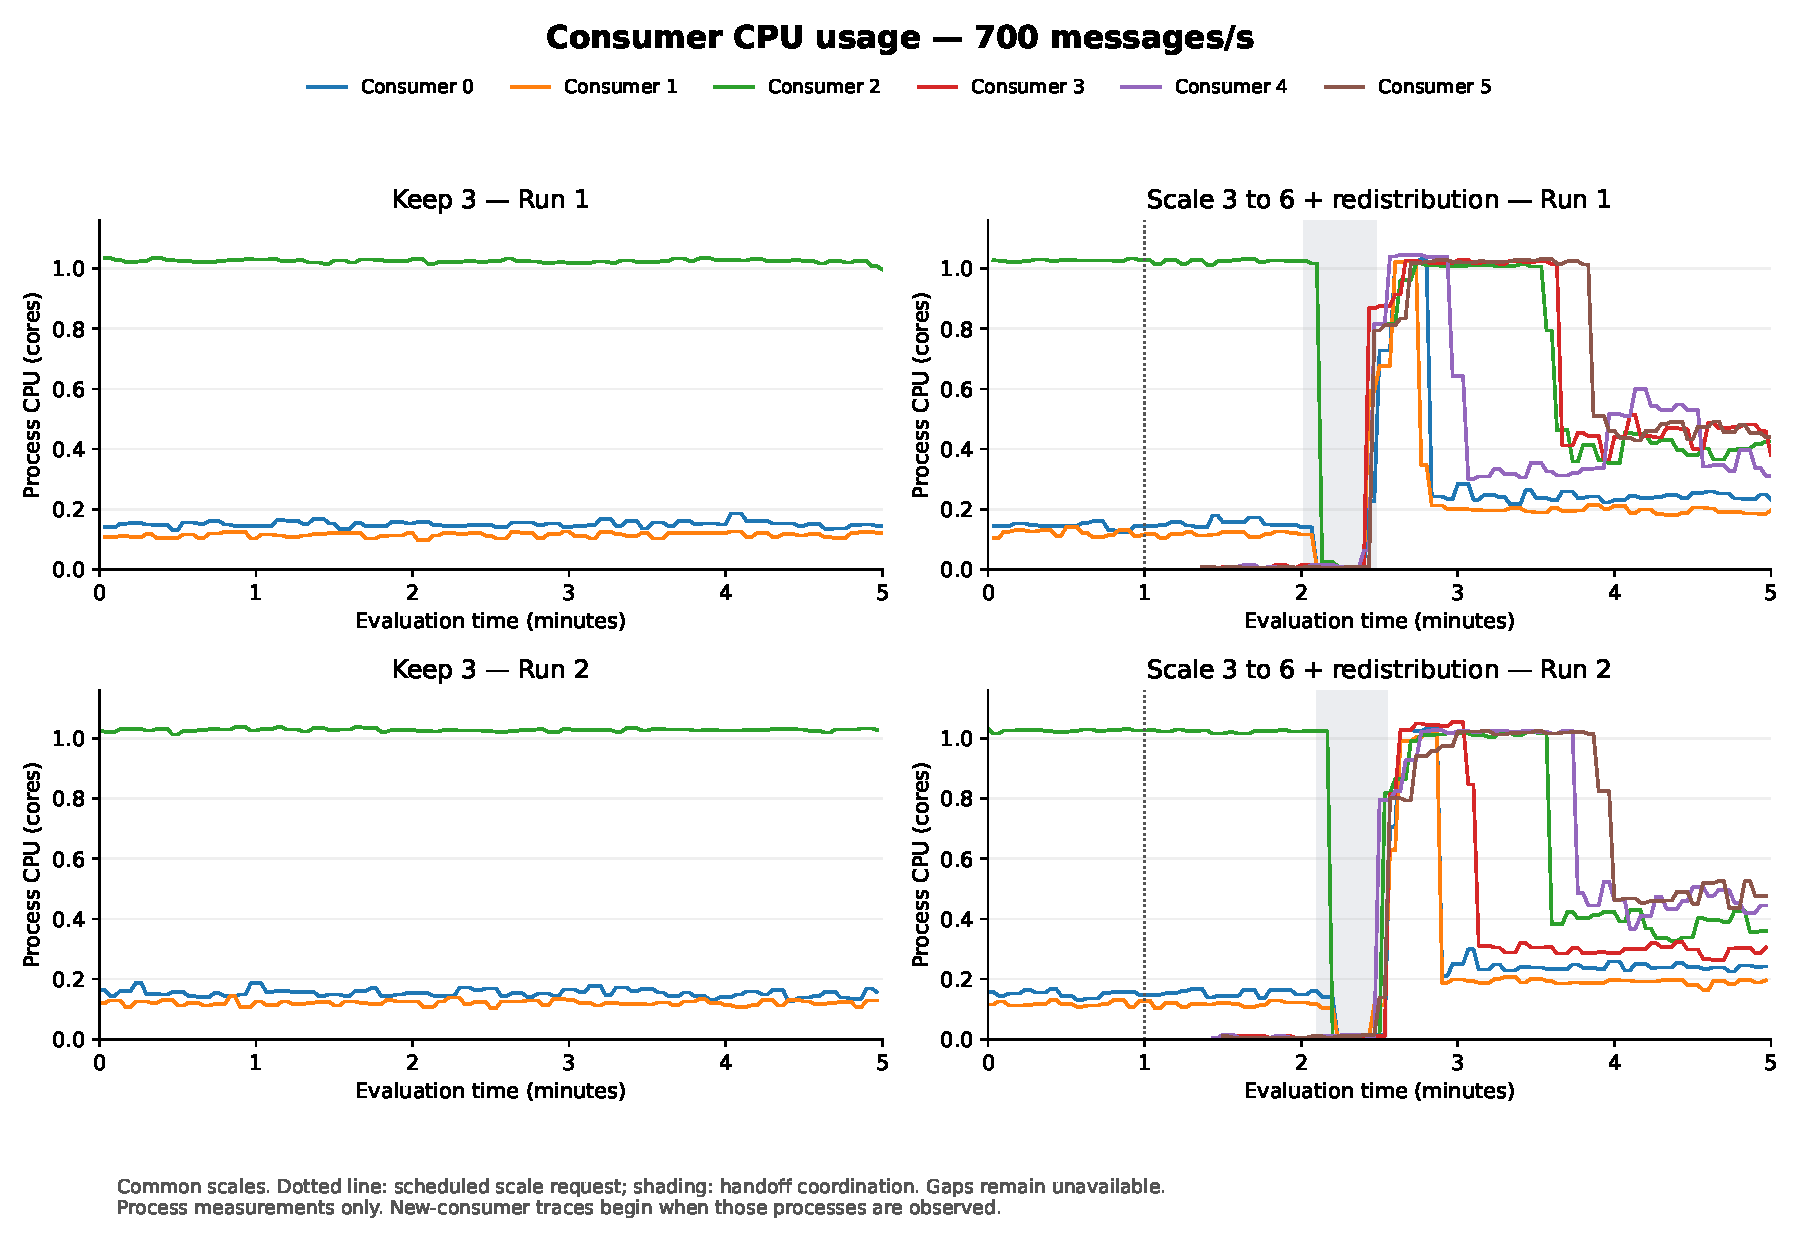
\includegraphics[width=\linewidth,height=5.25in,keepaspectratio]{figures/c2-scaling-cpu.pdf}
\caption{Adding consumers with explicit redistribution: consumer-process CPU use. CPU use is expressed in cores; one core corresponds to 100\% process CPU. It is distinct from requested CPU and excludes whole-node, broker, and producer use. Each panel covers five minutes of evaluation within an eight-minute trial.}
\label{fig:c2-scaling-cpu}
\end{figure}
\end{landscape}
\clearpage
\begin{landscape}
\begin{figure}[p]
\centering
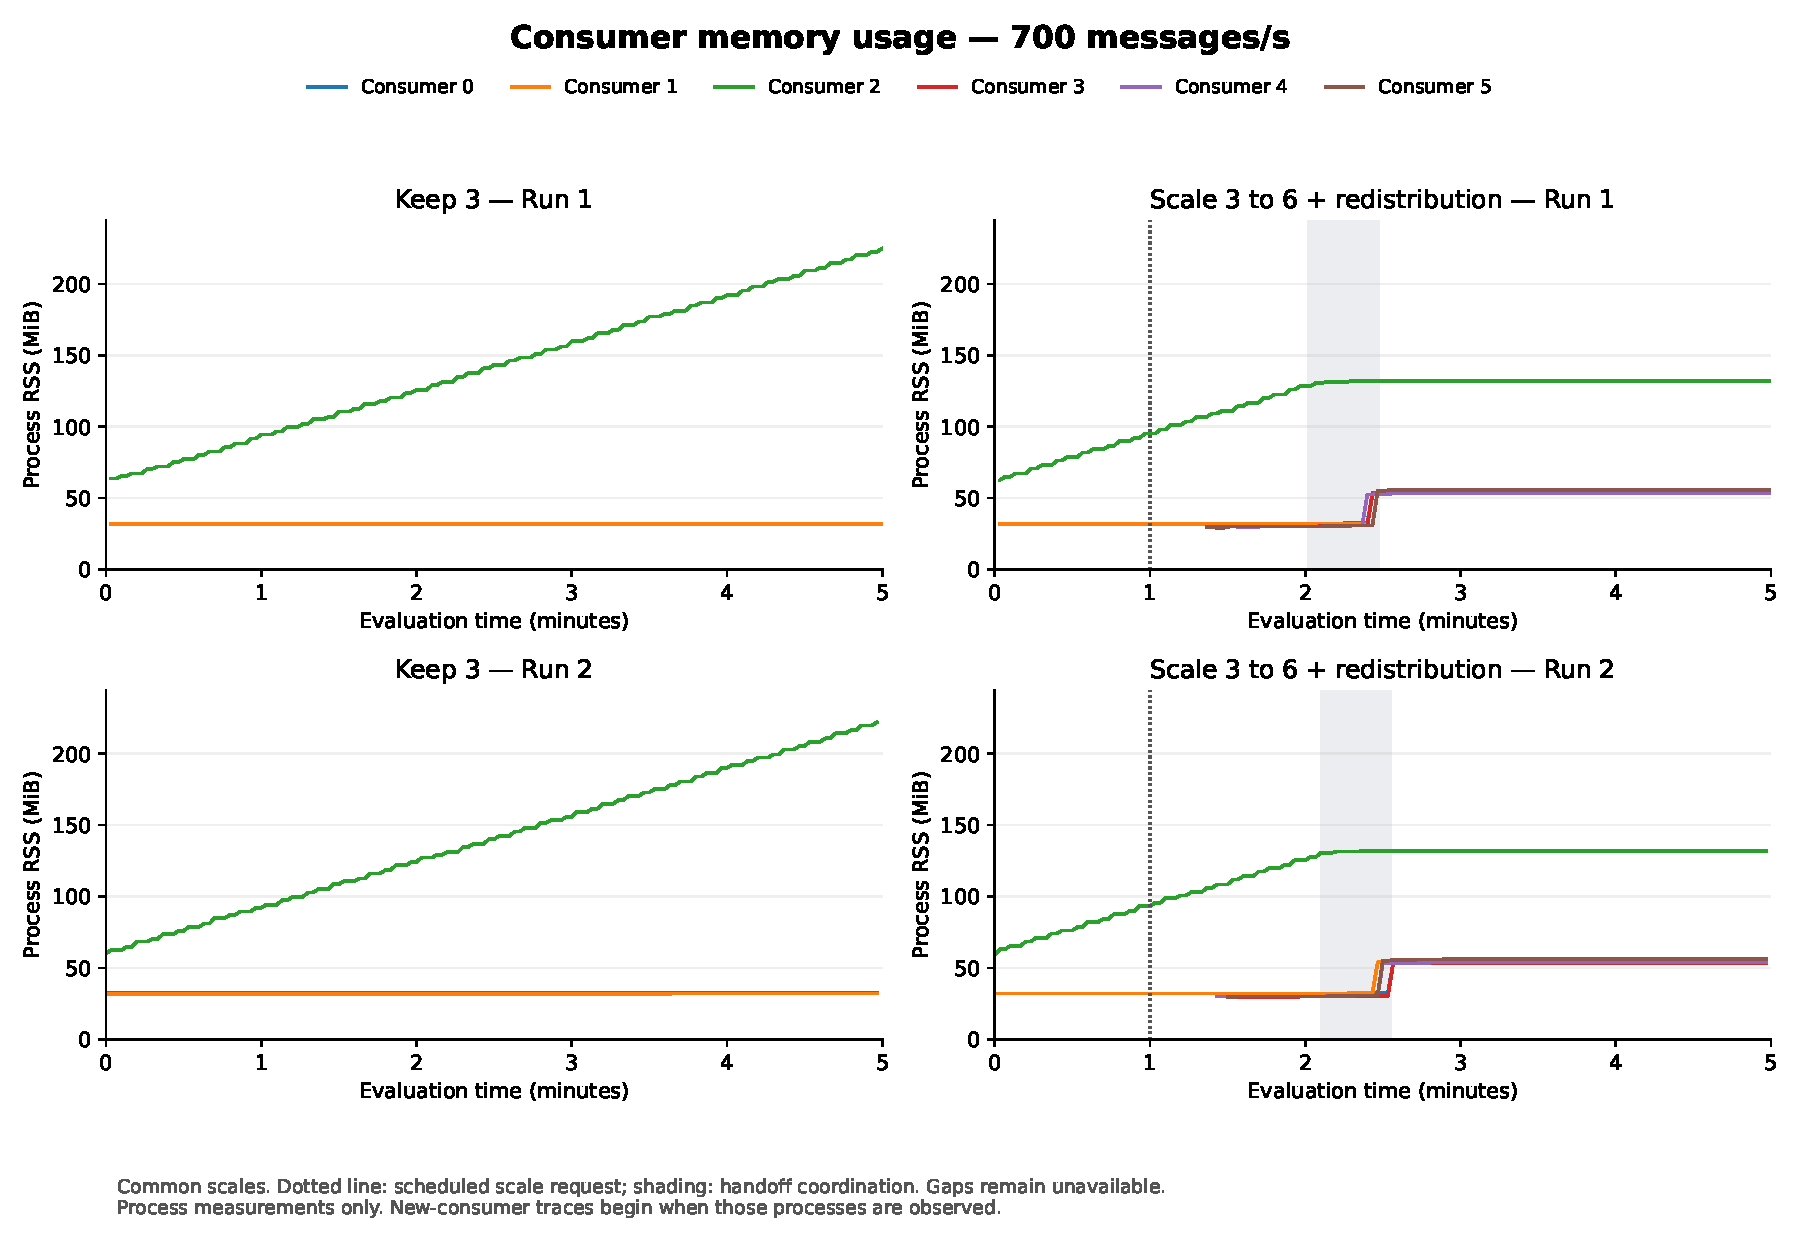
\includegraphics[width=\linewidth,height=5.25in,keepaspectratio]{figures/c2-scaling-memory.pdf}
\caption{Adding consumers with explicit redistribution: consumer-process resident memory. Resident set size measures the memory held by each consumer process. It is not the Kubernetes memory request, a transfer-volume measurement or a monetary cost. Each panel covers five minutes of evaluation within an eight-minute trial.}
\label{fig:c2-scaling-memory}
\end{figure}
\end{landscape}
\clearpage
\begin{landscape}
\begin{figure}[p]
\centering
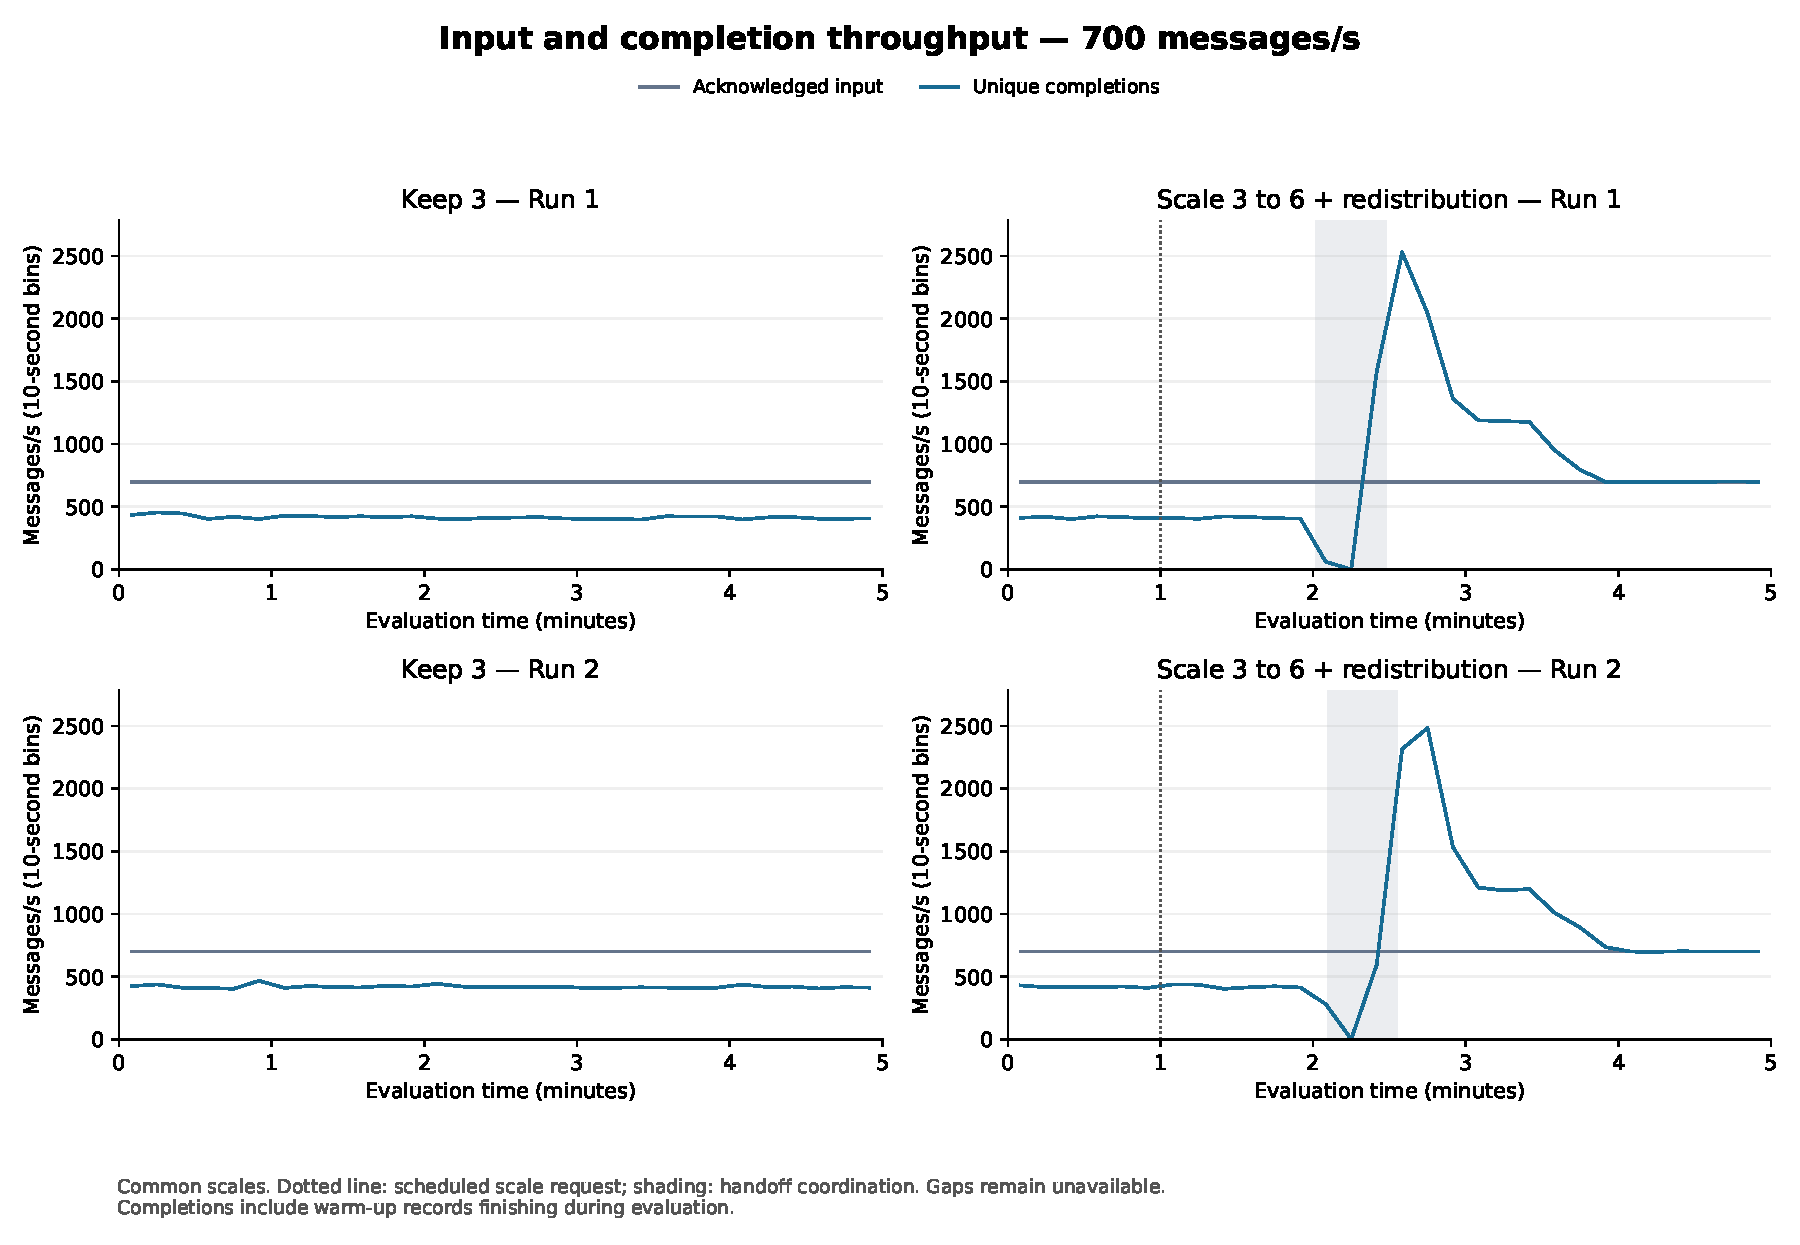
\includegraphics[width=\linewidth,height=5.25in,keepaspectratio]{figures/c2-scaling-throughput.pdf}
\caption{Adding consumers with explicit redistribution: acknowledged input and distinct completion throughput. Ten-second bins show input and processing progress. Completions can include queued warm-up messages, so catch-up throughput can exceed the 700-message/s input rate. Each panel covers five minutes of evaluation within an eight-minute trial.}
\label{fig:c2-scaling-throughput}
\end{figure}
\end{landscape}
\clearpage
\begin{landscape}
\begin{figure}[p]
\centering
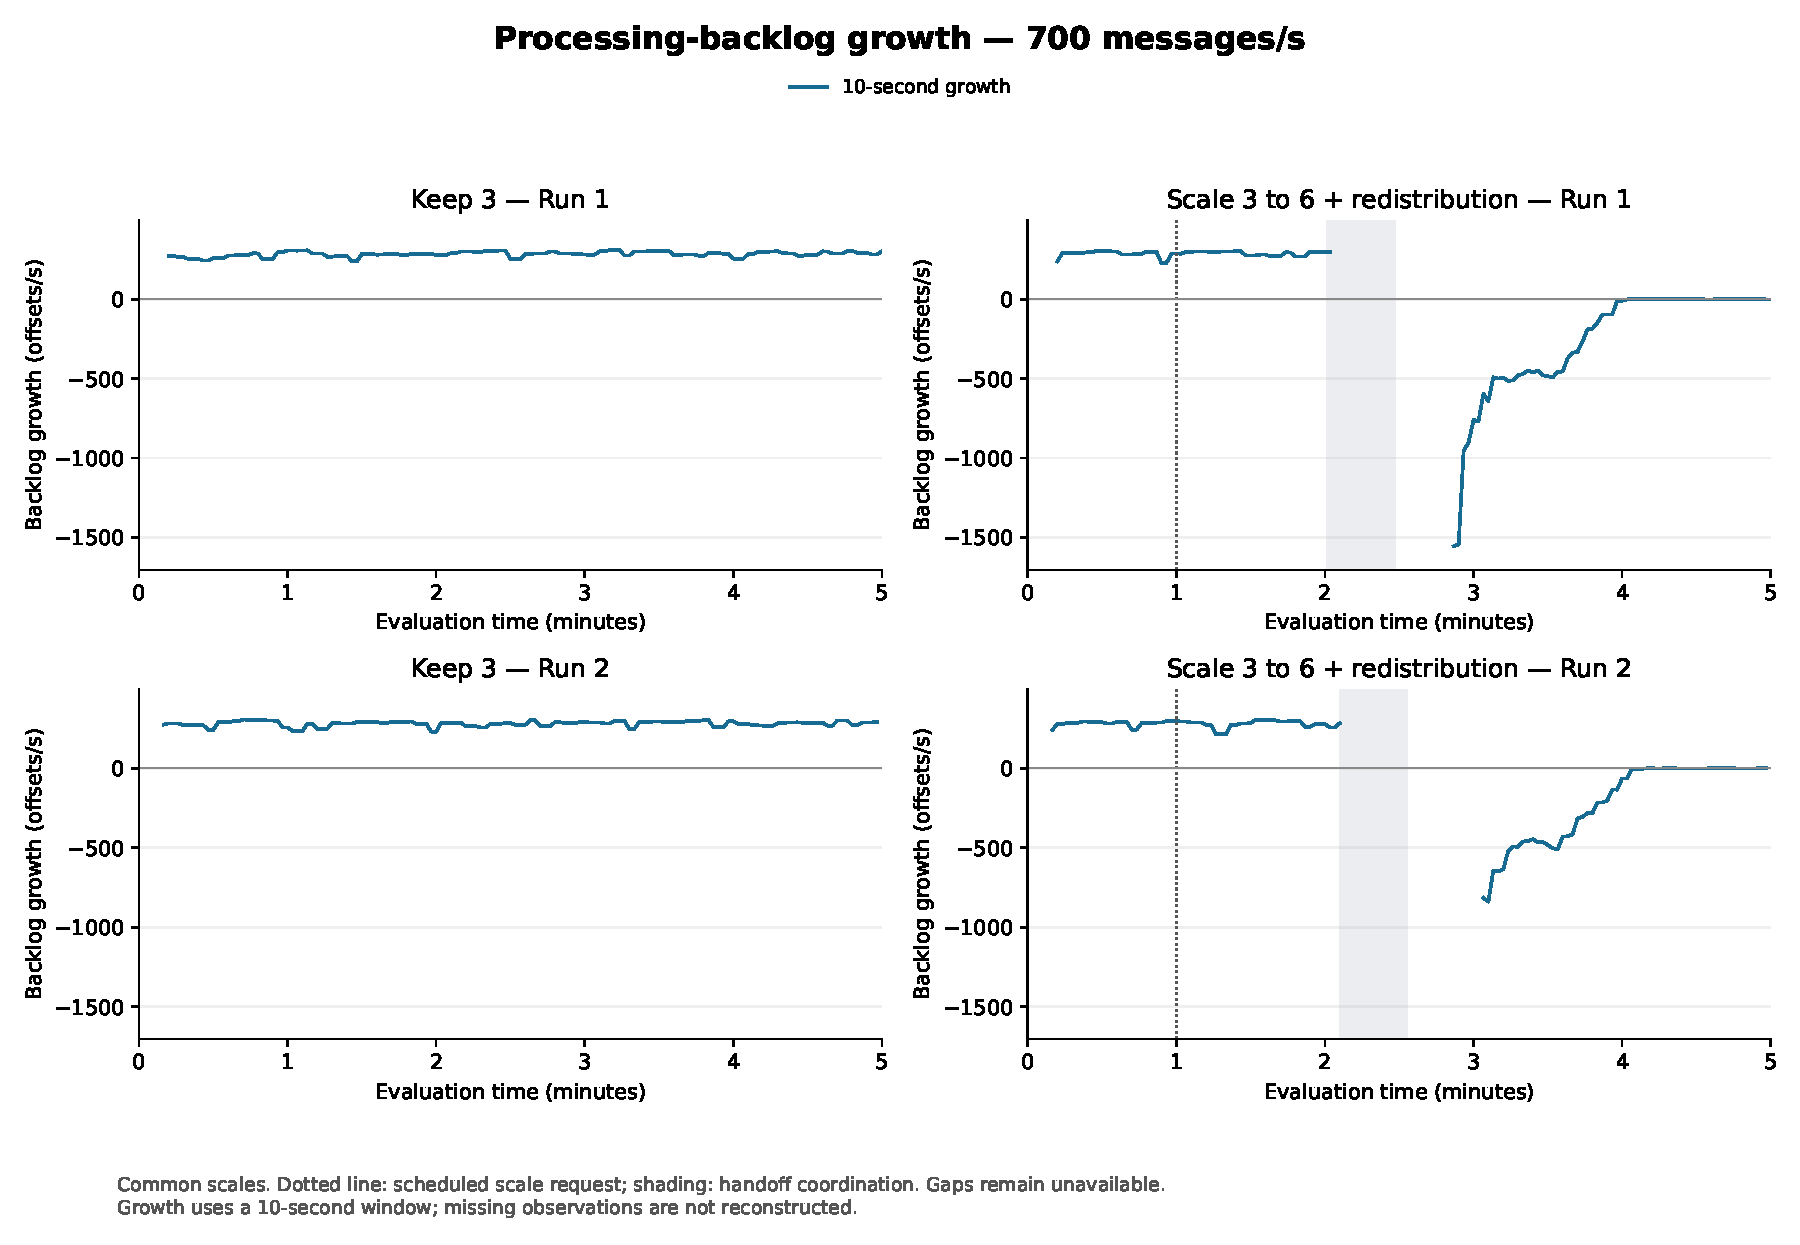
\includegraphics[width=\linewidth,height=5.10in,keepaspectratio]{figures/c2-scaling-growth.pdf}
\caption{Adding consumers with explicit redistribution: processing-backlog growth. Growth uses the position up to which all preceding messages have completed, measured over a ten-second window, shortened from thirty seconds after the trials and applied consistently across this block. Negative values indicate catch-up, not necessarily an empty backlog. Invalid intervals and ownership or offset resets are not bridged; a complete valid window is required before growth resumes. The separate requirement for thirty seconds of low backlog before confirming recovery is unchanged. Each panel covers five minutes of evaluation within an eight-minute trial.}
\label{fig:c2-scaling-growth}
\end{figure}
\end{landscape}
\clearpage
\begin{landscape}
\begin{figure}[p]
\centering
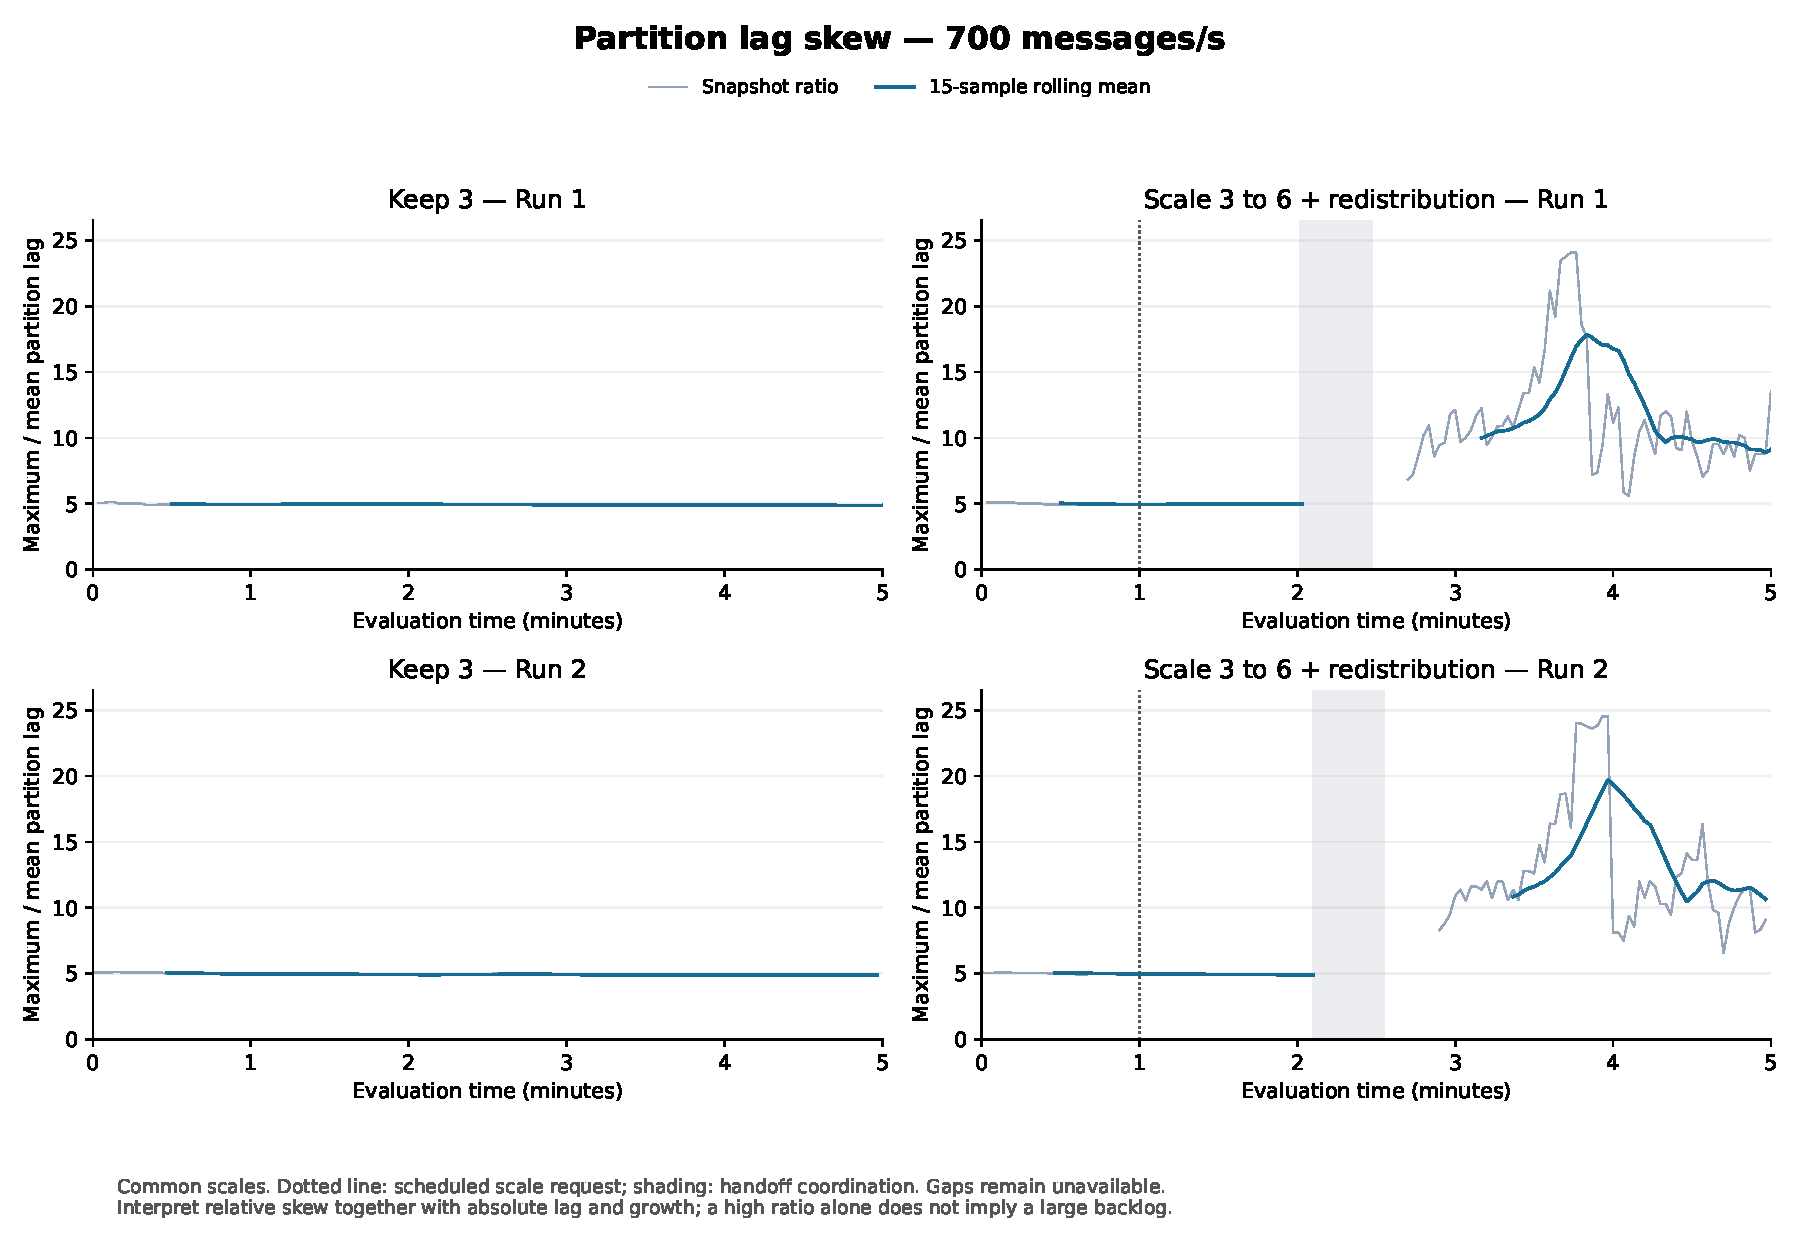
\includegraphics[width=\linewidth,height=5.25in,keepaspectratio]{figures/c2-scaling-skew.pdf}
\caption{Adding consumers with explicit redistribution: partition-level lag skew. The maximum-to-mean ratio is interpreted with absolute lag and growth. A high relative ratio alone does not establish severe overload; a ratio near one can also coexist with broadly distributed backlog. Each panel covers five minutes of evaluation within an eight-minute trial.}
\label{fig:c2-scaling-skew}
\end{figure}
\end{landscape}
\clearpage

\clearpage
\begin{landscape}
\begin{figure}[p]
\centering
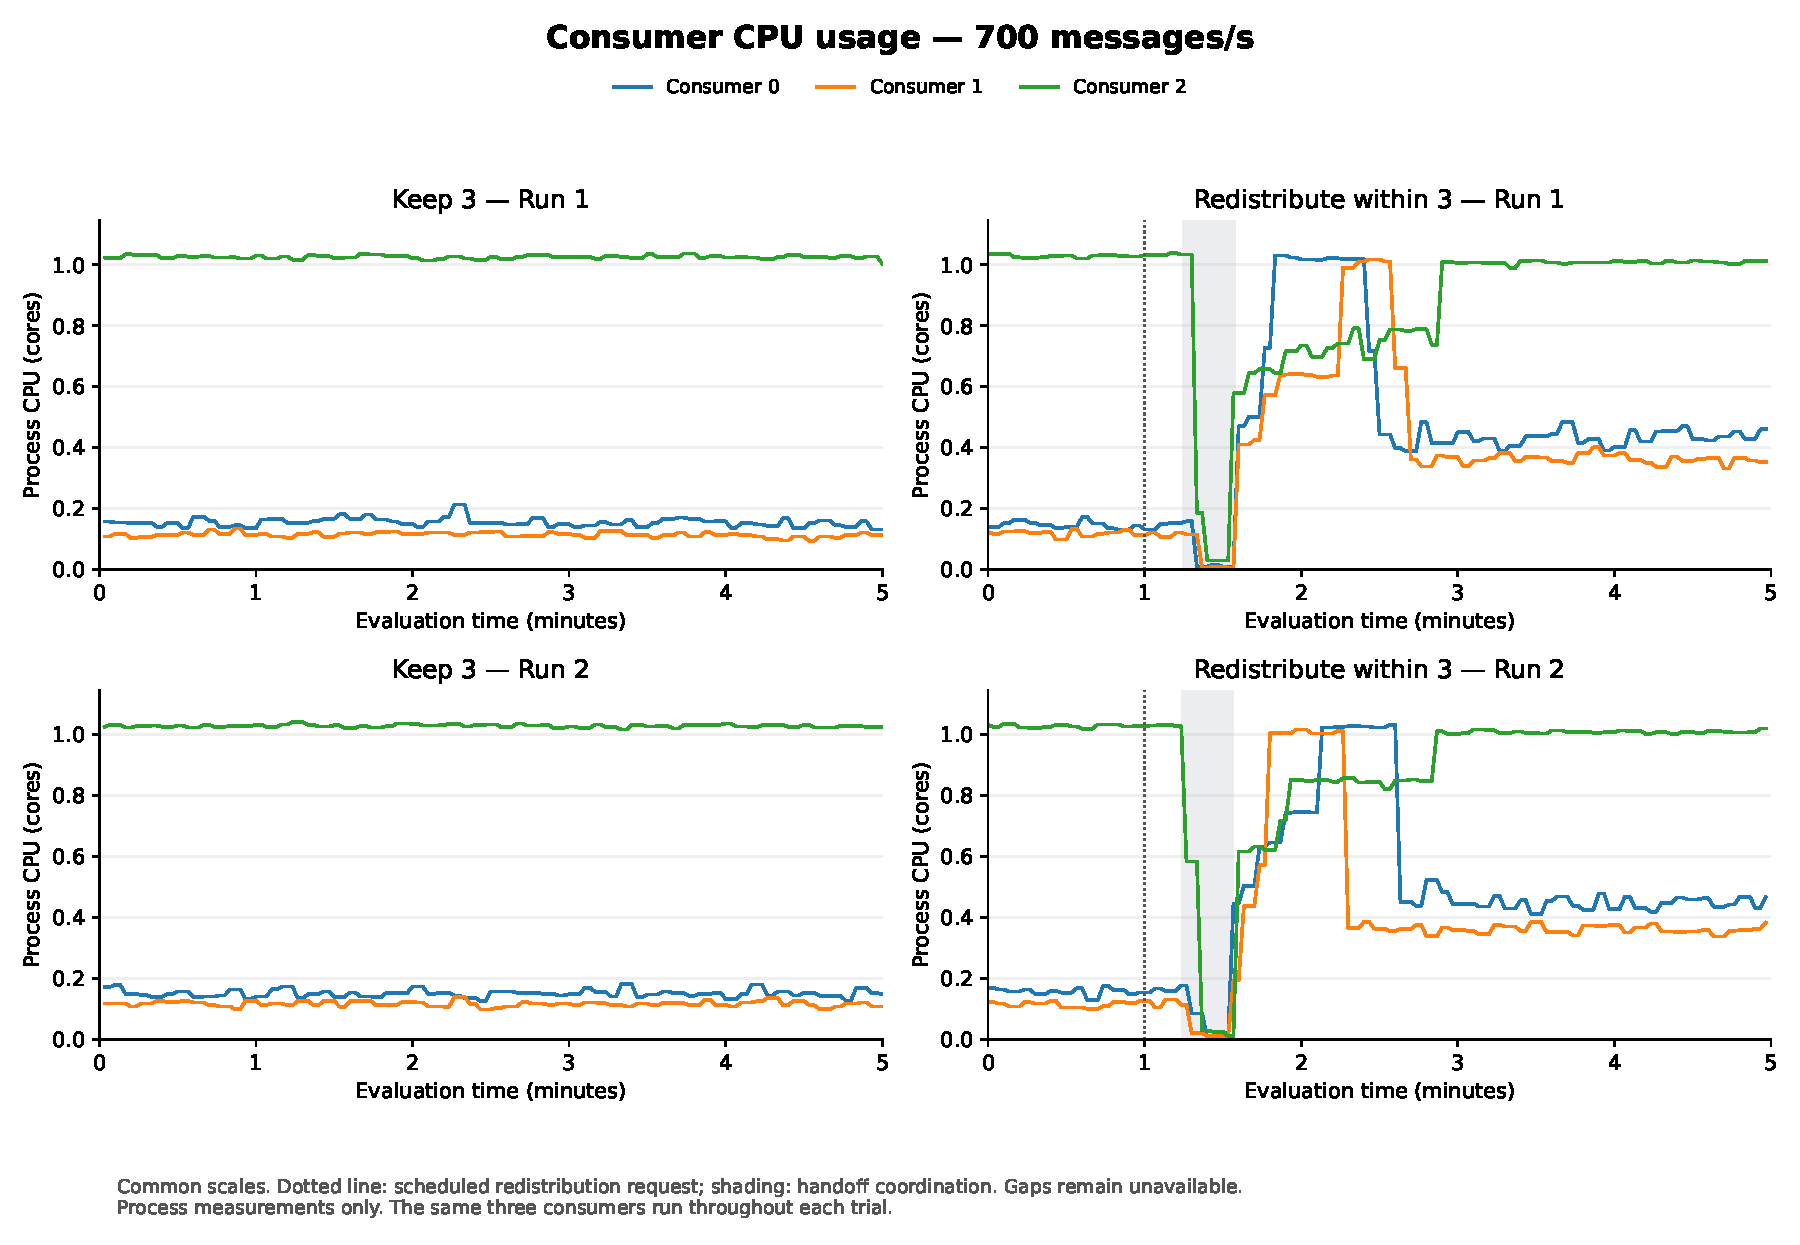
\includegraphics[width=\linewidth,height=5.25in,keepaspectratio]{figures/c2-redistribution-cpu.pdf}
\caption{Redistribution within three consumers: consumer-process CPU use. CPU use is expressed in cores; one core corresponds to 100\% process CPU. It is distinct from requested CPU and excludes whole-node, broker and producer use. Each panel covers five minutes of evaluation within an eight-minute trial.}
\label{fig:c2-redistribution-cpu}
\end{figure}
\end{landscape}
\clearpage
\begin{landscape}
\begin{figure}[p]
\centering
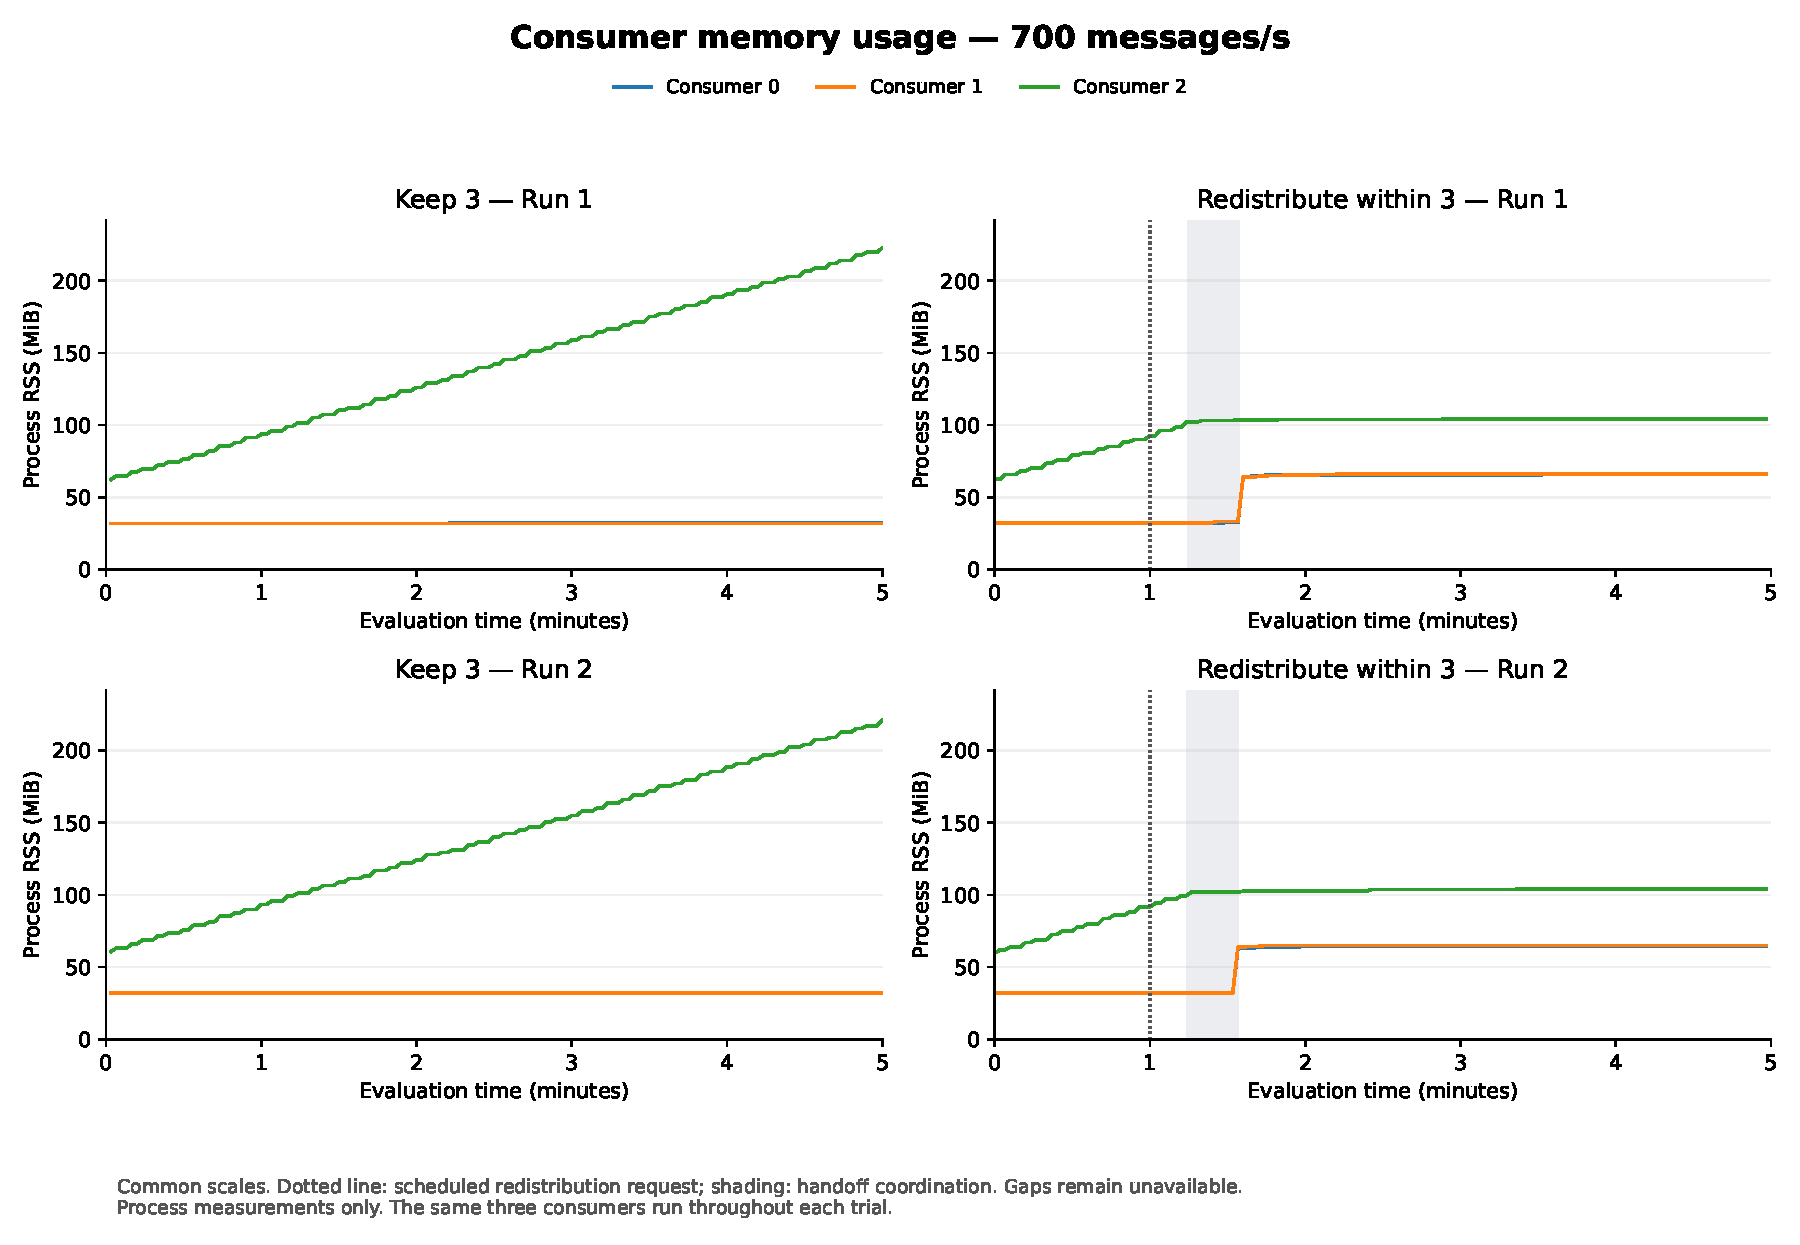
\includegraphics[width=\linewidth,height=5.25in,keepaspectratio]{figures/c2-redistribution-memory.pdf}
\caption{Redistribution within three consumers: consumer-process resident memory. Resident set size measures the memory held by each consumer process. It is not the Kubernetes memory request, a transfer-volume measurement or a monetary cost. Each panel covers five minutes of evaluation within an eight-minute trial.}
\label{fig:c2-redistribution-memory}
\end{figure}
\end{landscape}
\clearpage
\begin{landscape}
\begin{figure}[p]
\centering
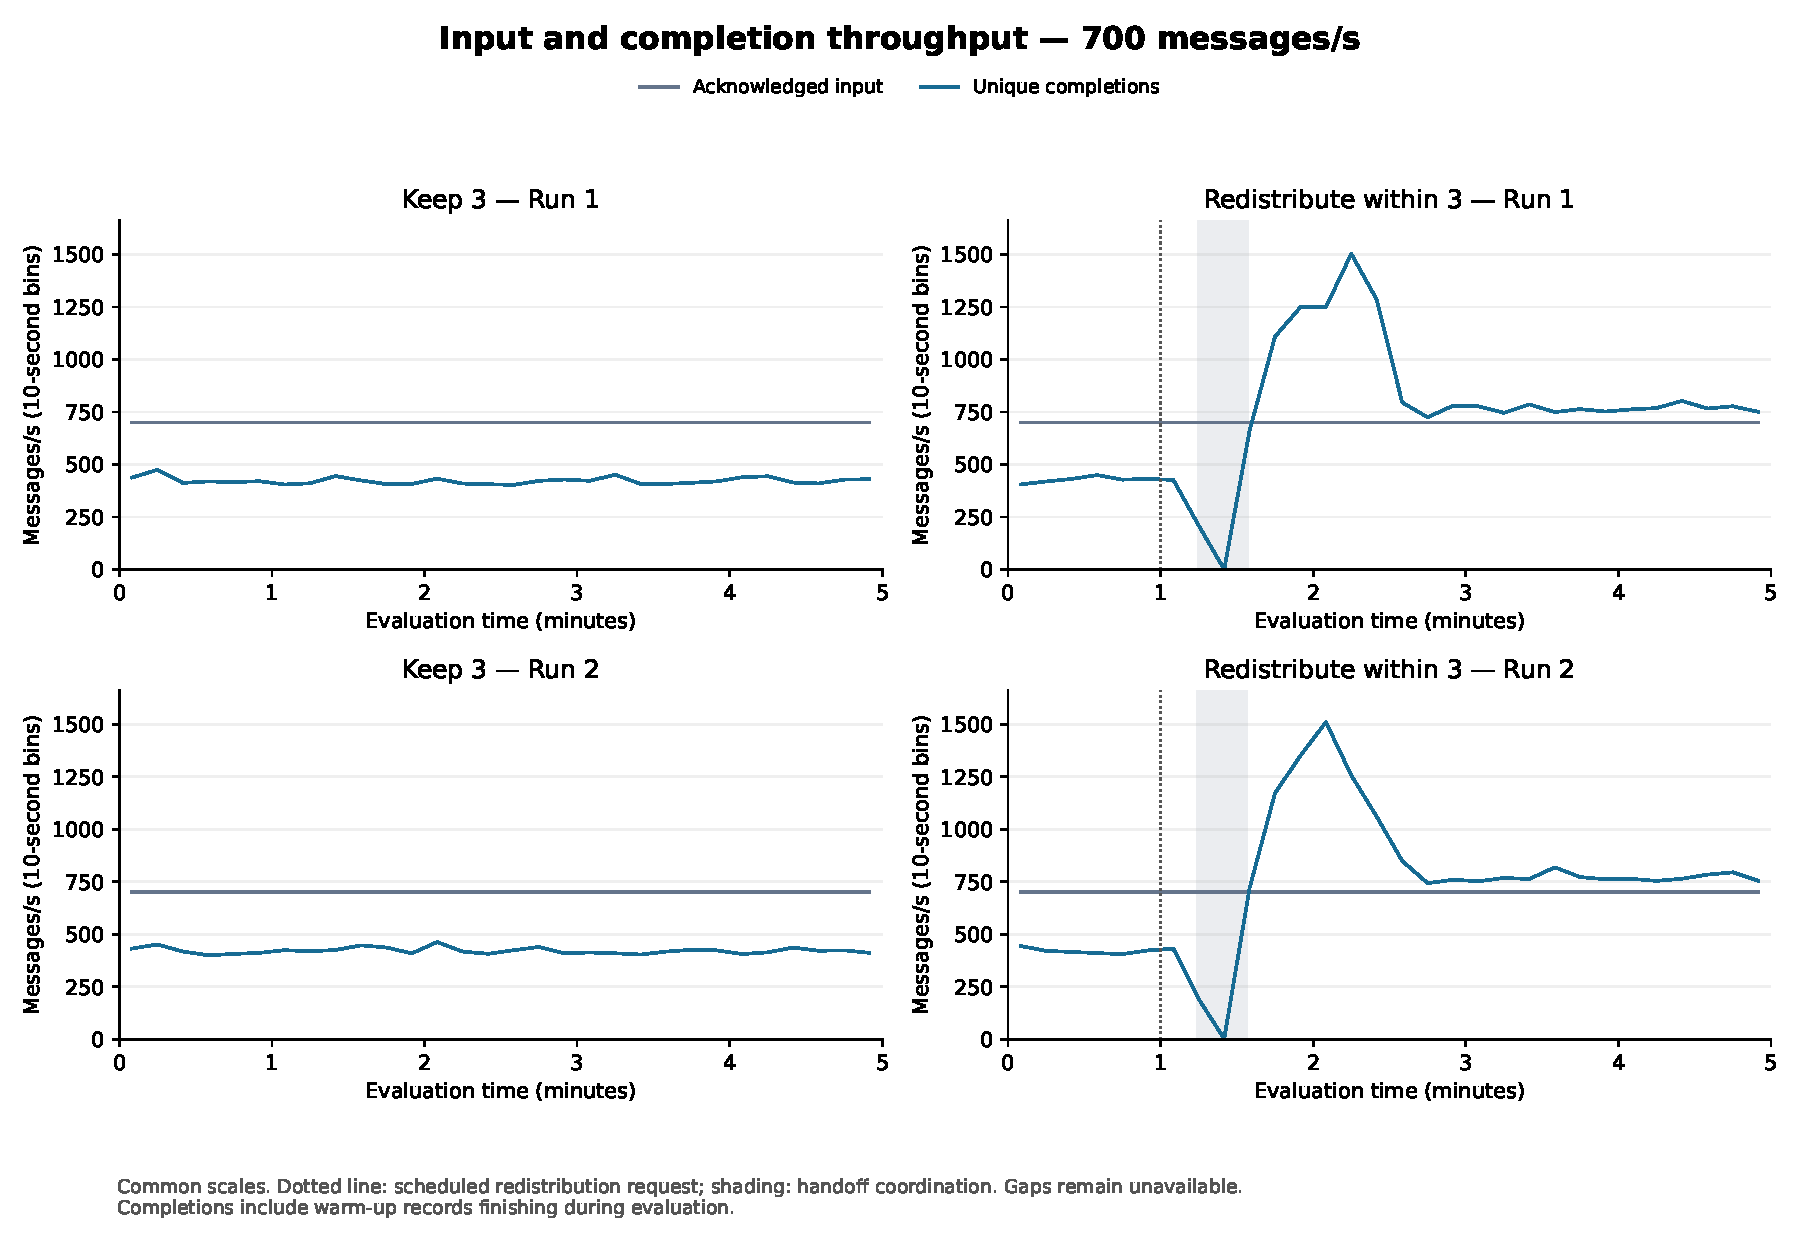
\includegraphics[width=\linewidth,height=5.25in,keepaspectratio]{figures/c2-redistribution-throughput.pdf}
\caption{Redistribution within three consumers: acknowledged input and distinct completion throughput. Ten-second bins show input and processing progress. Completions can include queued warm-up messages, so catch-up throughput can exceed the 700-message/s input rate. Each panel covers five minutes of evaluation within an eight-minute trial.}
\label{fig:c2-redistribution-throughput}
\end{figure}
\end{landscape}
\clearpage
\begin{landscape}
\begin{figure}[p]
\centering
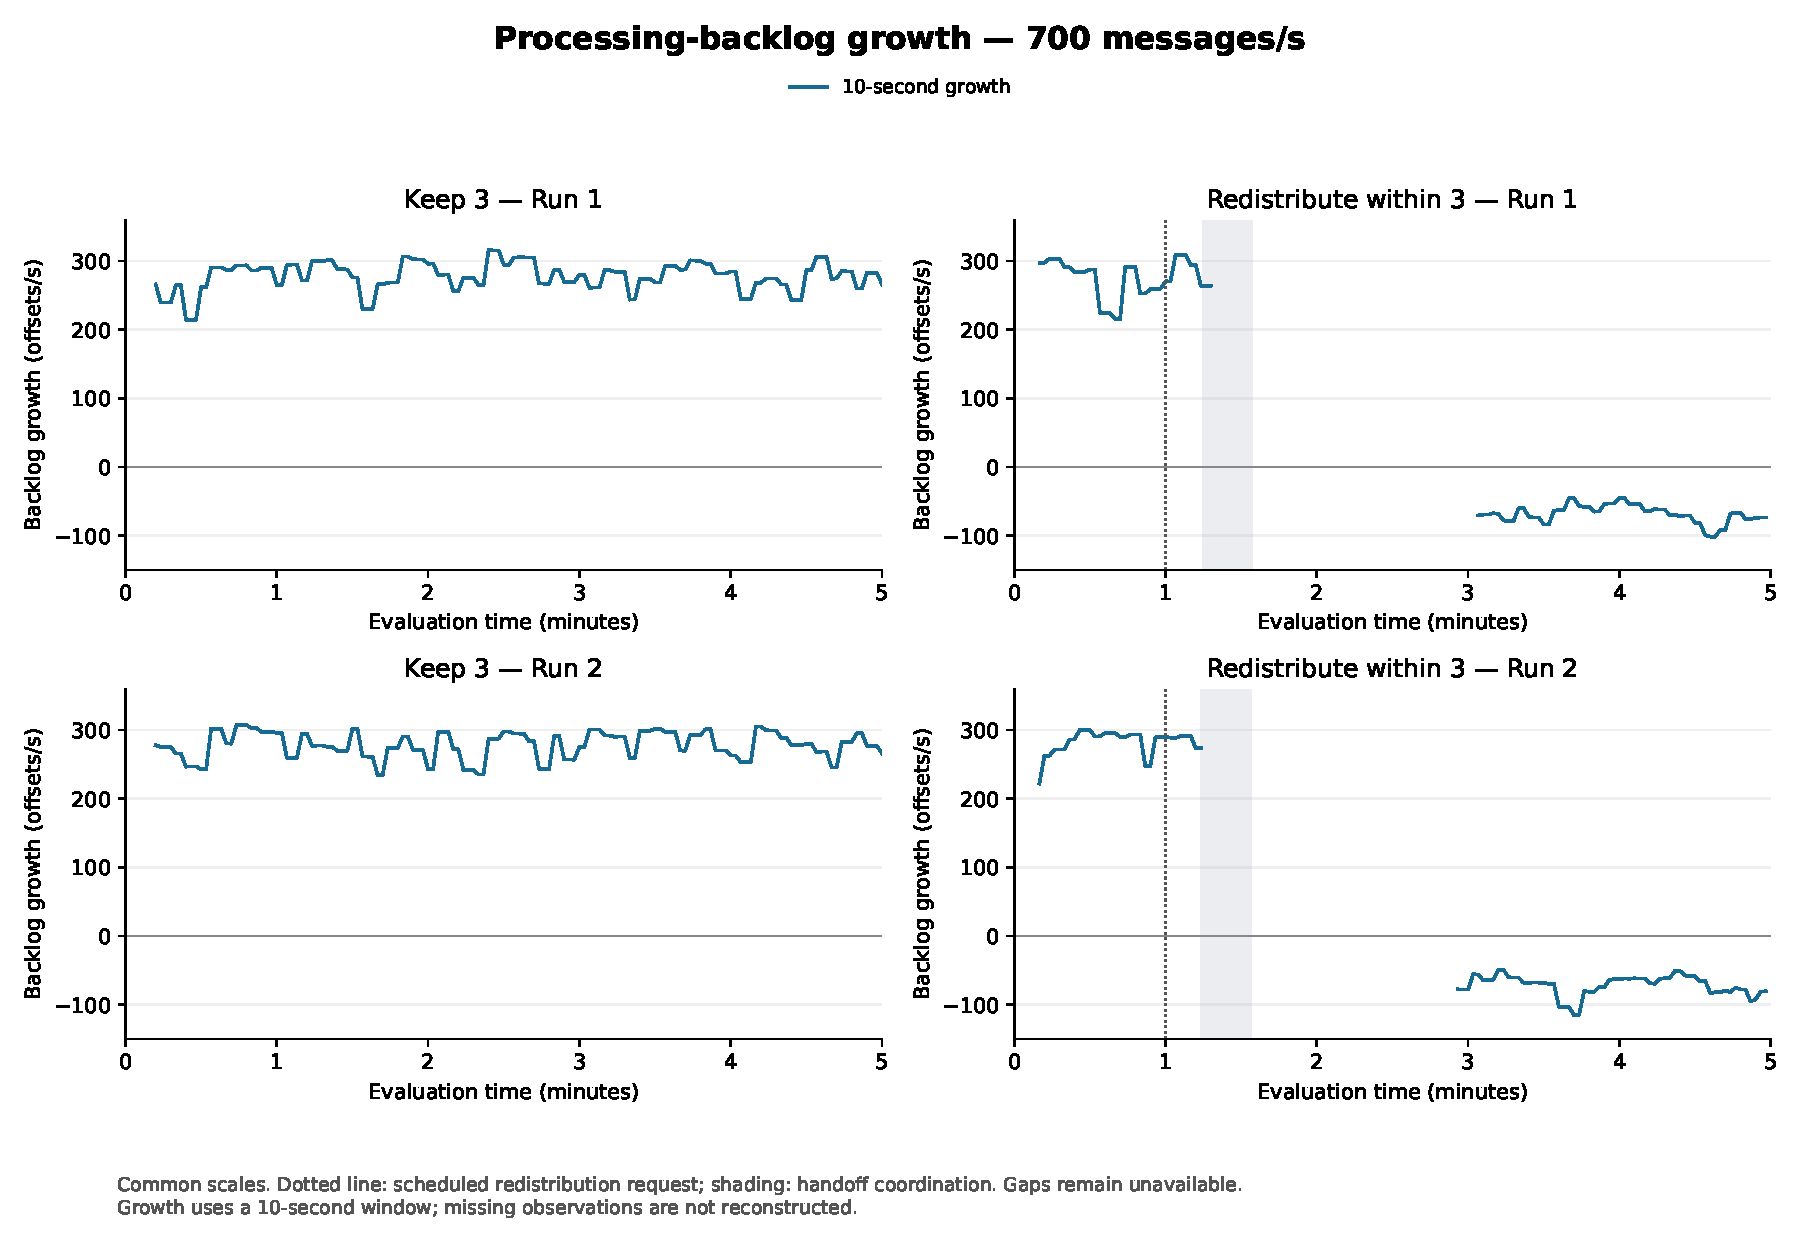
\includegraphics[width=\linewidth,height=5.10in,keepaspectratio]{figures/c2-redistribution-growth.pdf}
\caption{Redistribution within three consumers: processing-backlog growth. Growth uses the position up to which all preceding messages have completed, measured over a ten-second window, shortened from thirty seconds after the trials and applied consistently across this block. Negative values indicate catch-up, not necessarily an empty backlog. Invalid intervals and ownership or offset resets are not bridged; a complete valid window is required before growth resumes. The separate requirement for thirty seconds of low backlog before confirming recovery is unchanged. Each panel covers five minutes of evaluation within an eight-minute trial.}
\label{fig:c2-redistribution-growth}
\end{figure}
\end{landscape}
\clearpage
\begin{landscape}
\begin{figure}[p]
\centering
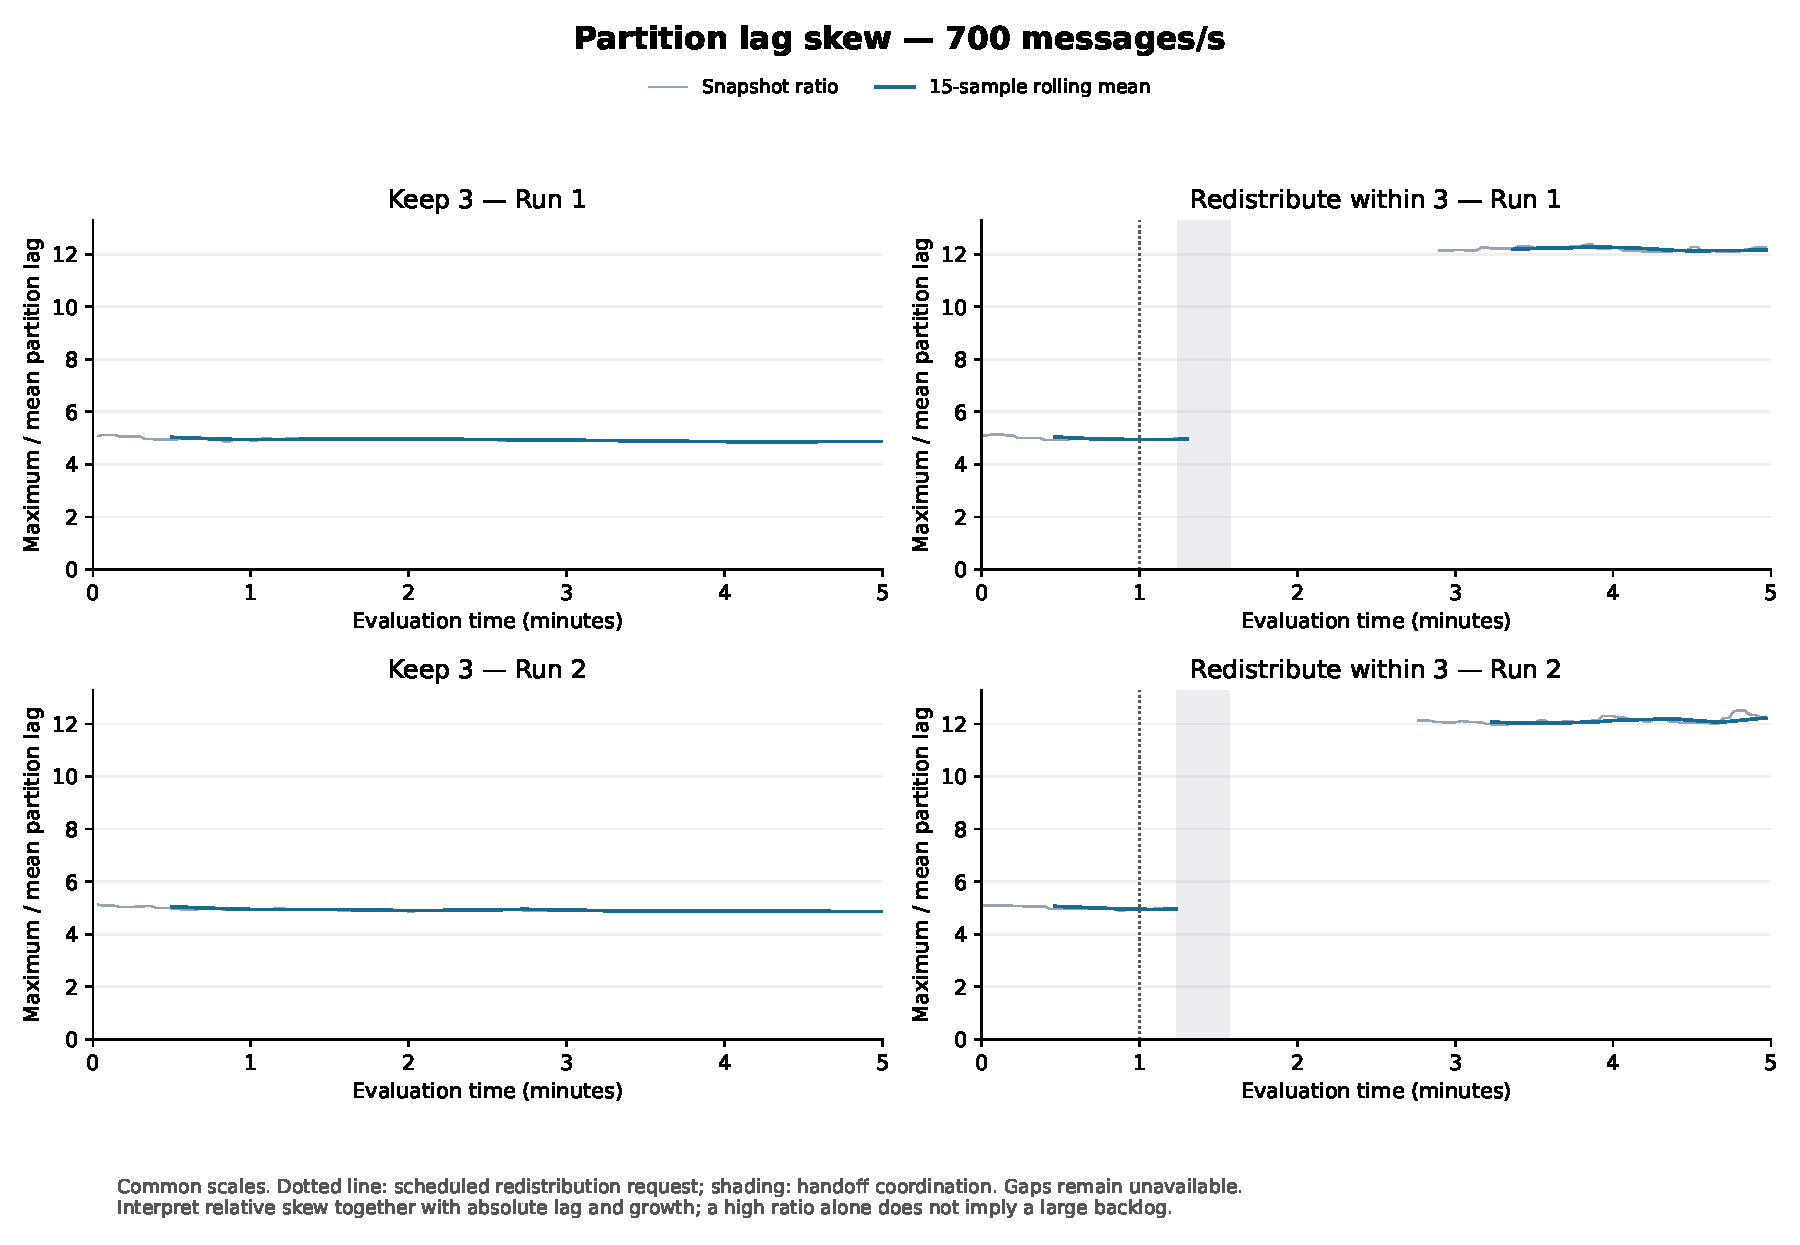
\includegraphics[width=\linewidth,height=5.25in,keepaspectratio]{figures/c2-redistribution-skew.pdf}
\caption{Redistribution within three consumers: partition-level lag skew. The maximum-to-mean ratio is interpreted with absolute lag and growth. A high relative ratio alone does not establish severe overload; a ratio near one can also coexist with broadly distributed backlog. Each panel covers five minutes of evaluation within an eight-minute trial.}
\label{fig:c2-redistribution-skew}
\end{figure}
\end{landscape}
\clearpage



\begin{landscape}
\begin{figure}[p]
\centering
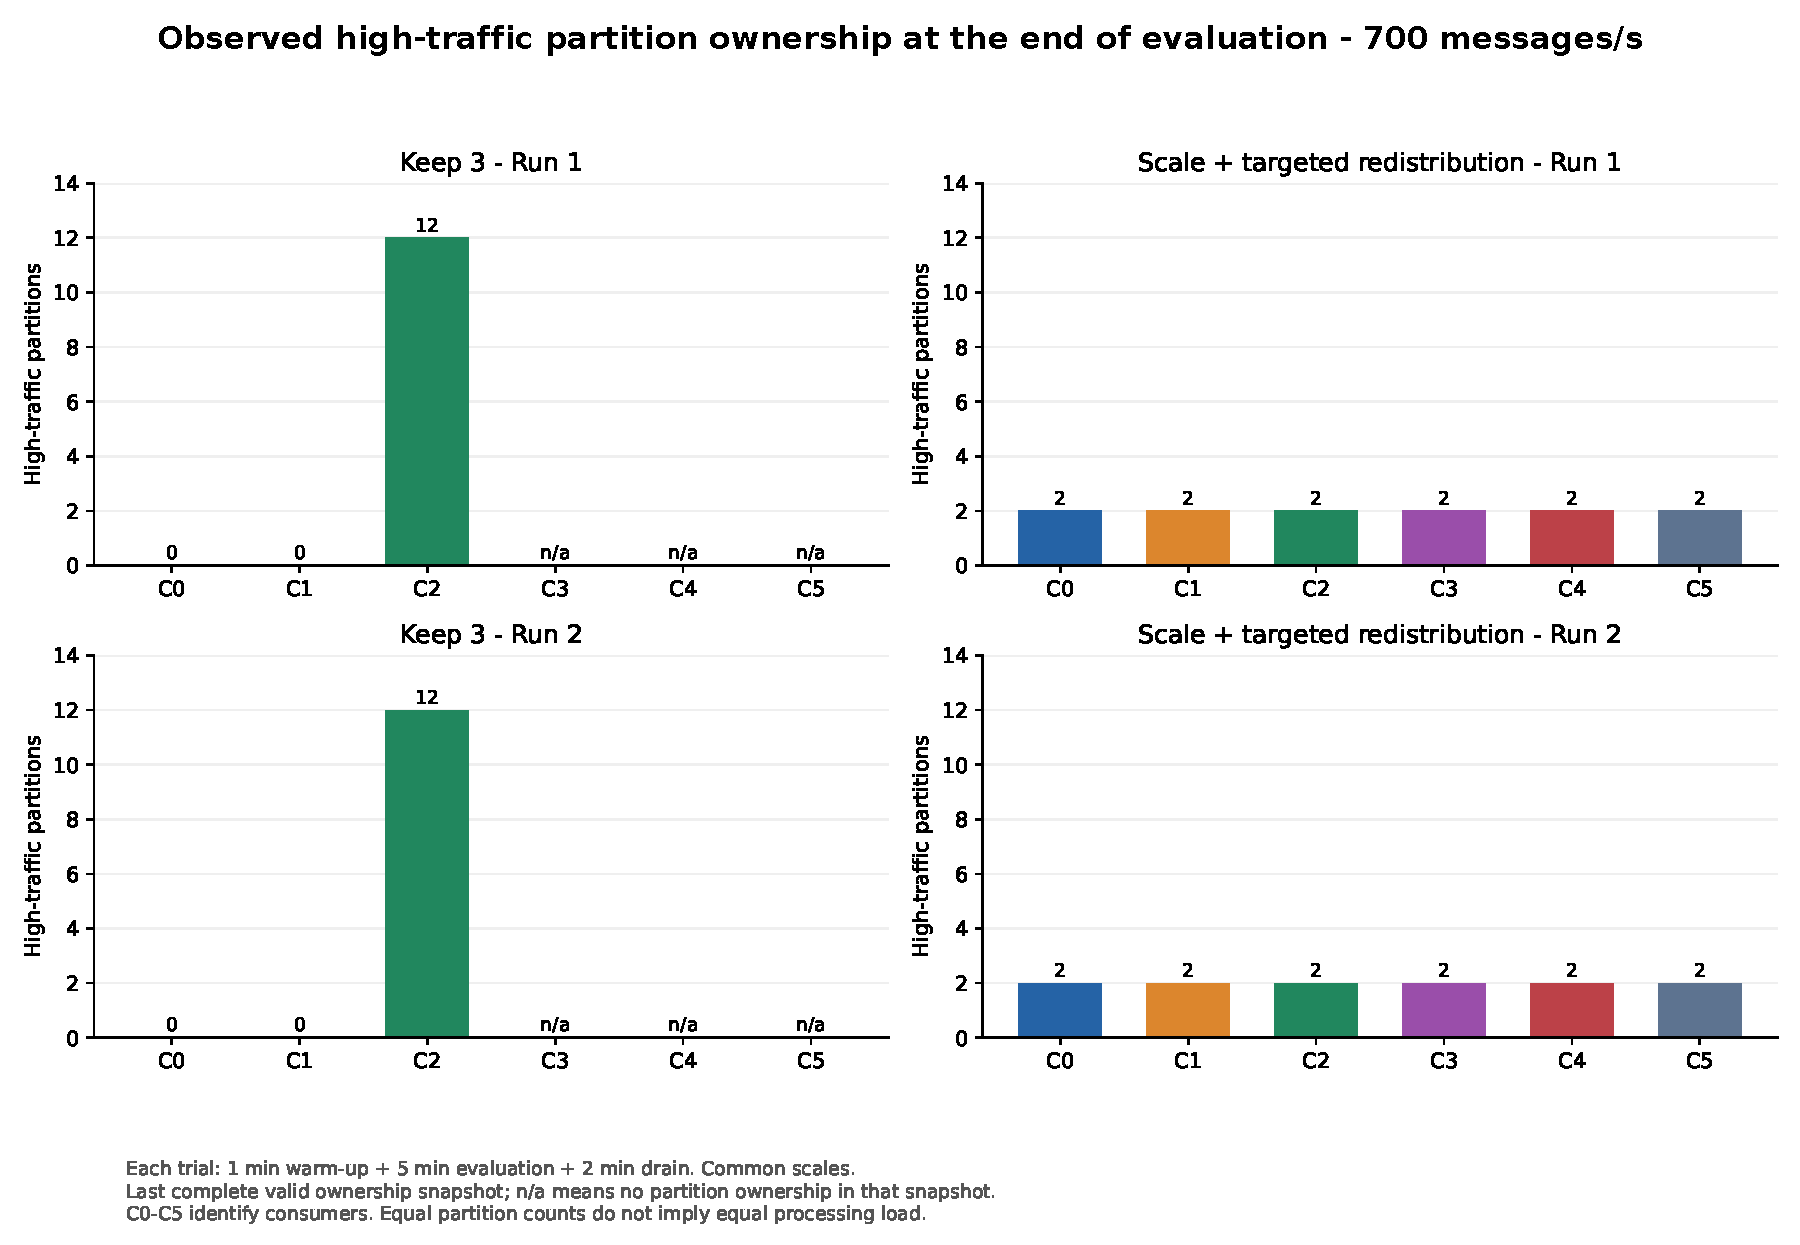
\includegraphics[width=\linewidth,height=5.1in,keepaspectratio]{figures/c2-scaling-ownership.pdf}
\caption{Observed high-traffic partition ownership in the five-minute scaling-with-redistribution trials. Baselines retained all twelve on Consumer 2; targeted scaling placed two on each of six consumers. Equal partition counts do not establish equal load.}
\label{fig:c2-scaling-ownership}
\end{figure}
\end{landscape}
\clearpage

\begin{landscape}
\begin{figure}[p]
\centering
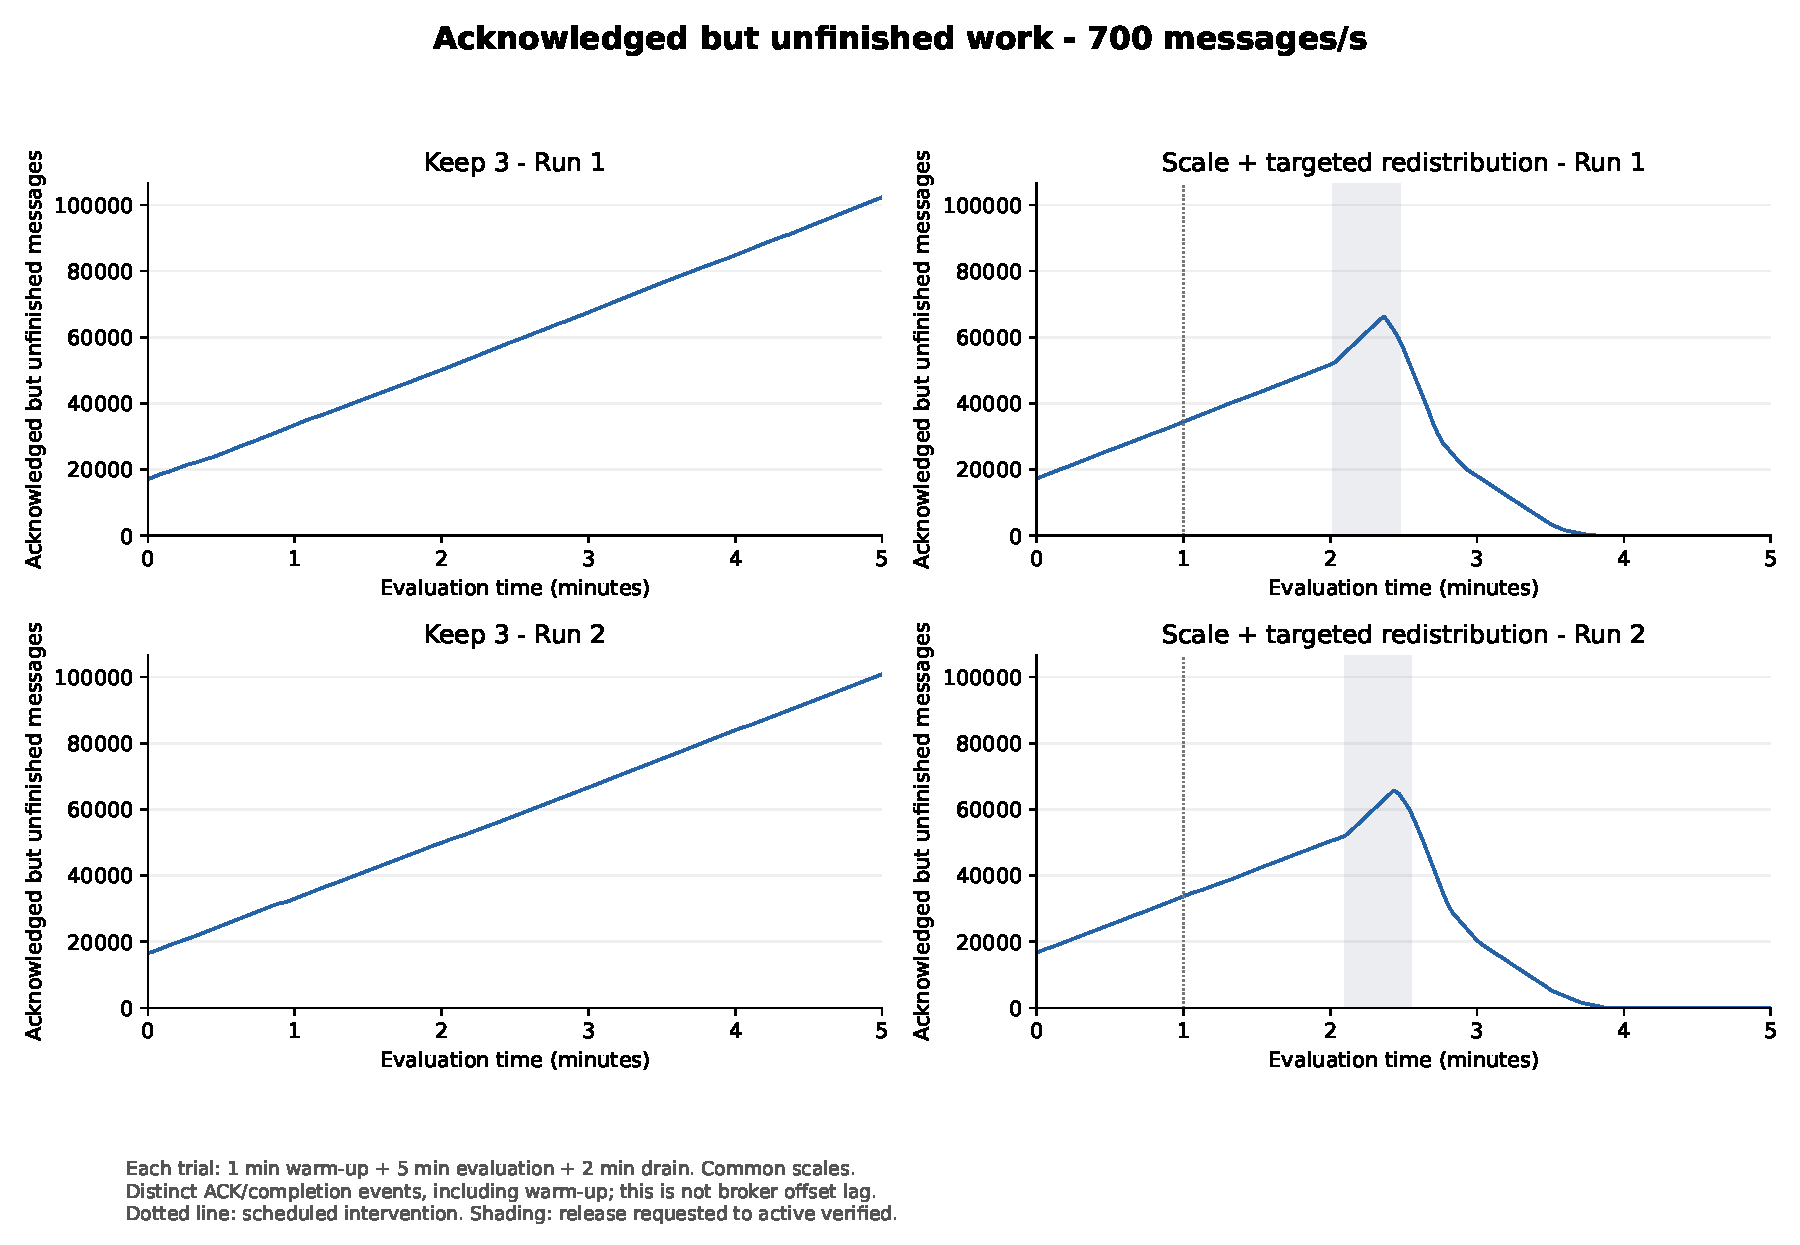
\includegraphics[width=\linewidth,height=5.1in,keepaspectratio]{figures/c2-scaling-outstanding.pdf}
\caption{Distinct acknowledged messages not yet completed during the five-minute scaling-with-redistribution trials, including warm-up work. The dotted line marks the scheduled intervention; shading spans release request to verified active ownership. Each full trial lasts eight minutes including warm-up and drain.}
\label{fig:c2-scaling-outstanding}
\end{figure}
\end{landscape}
\clearpage

\begin{landscape}
\begin{figure}[p]
\centering
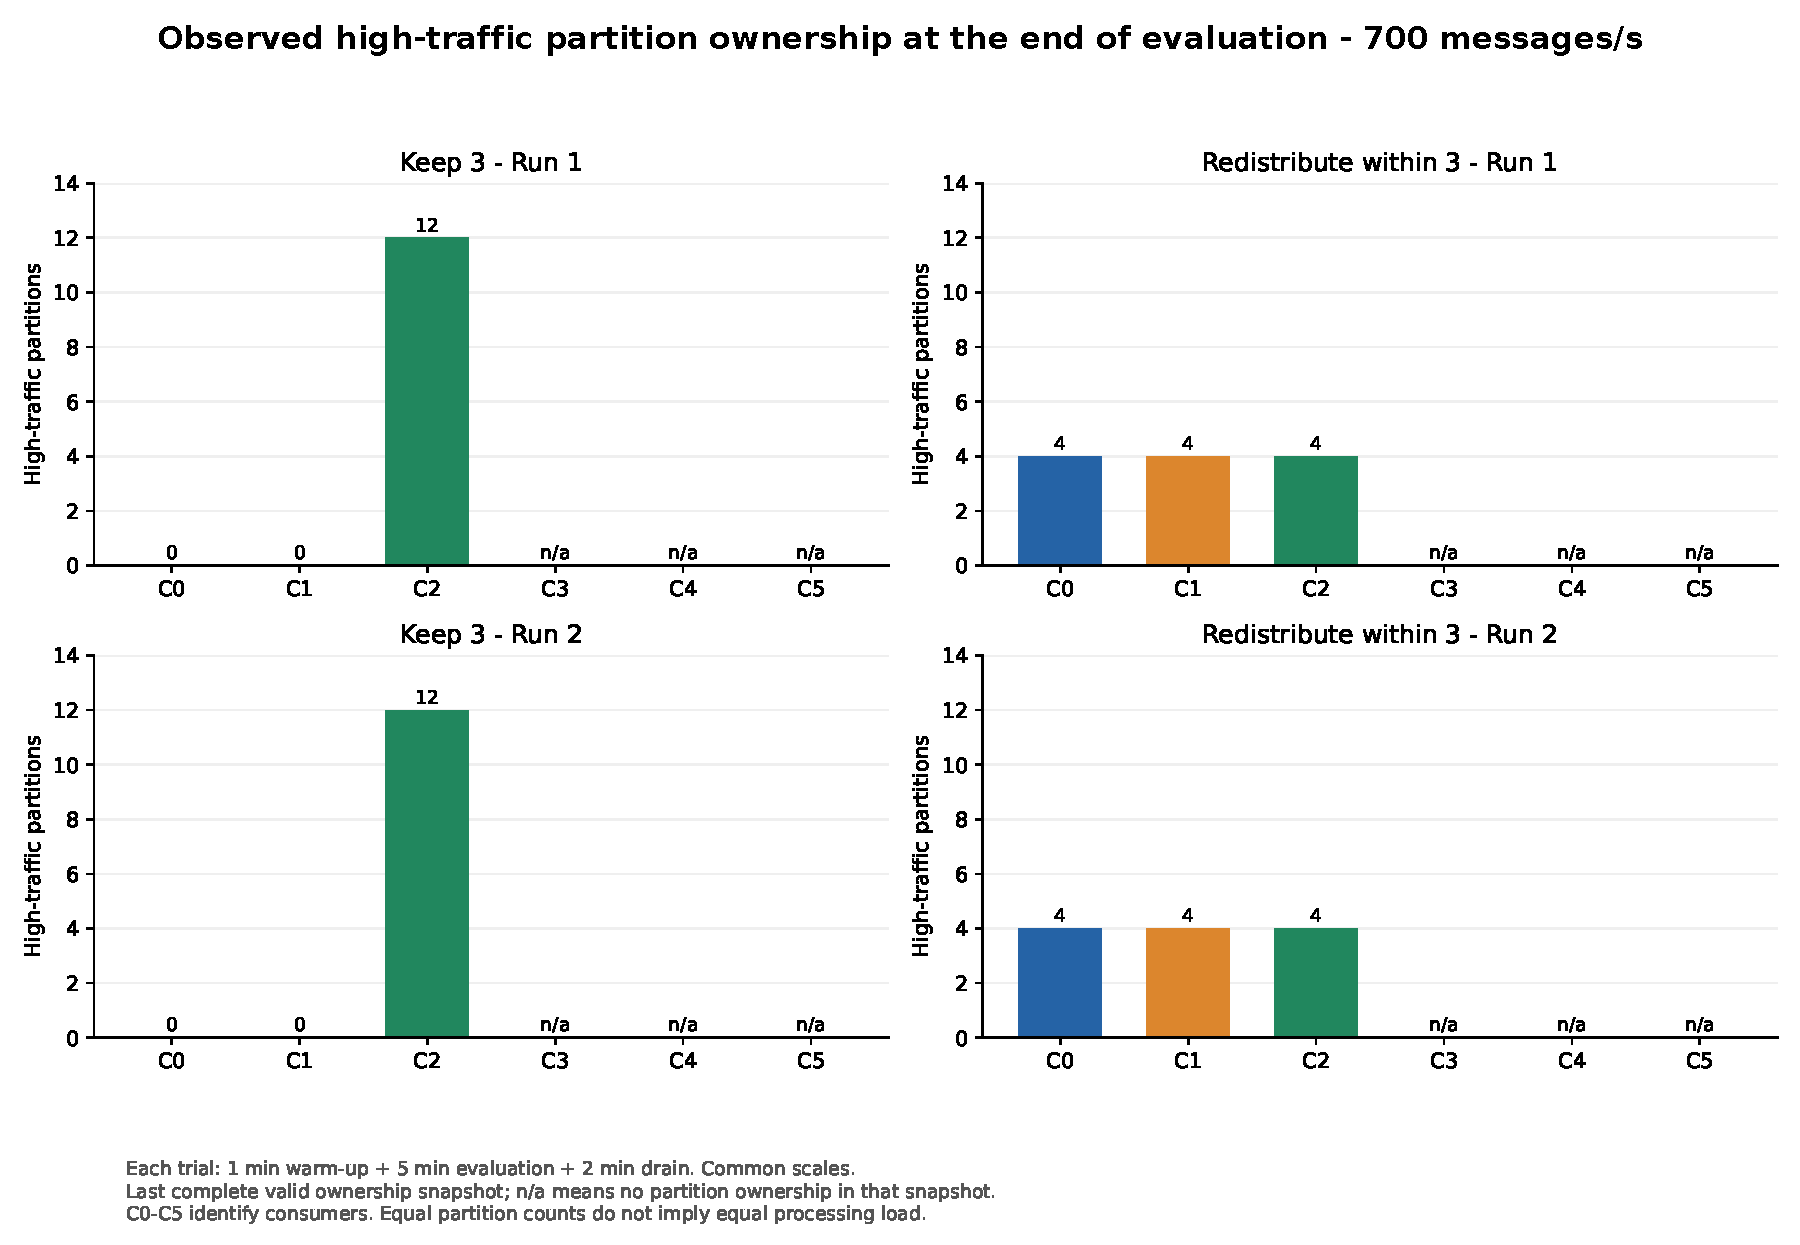
\includegraphics[width=\linewidth,height=5.1in,keepaspectratio]{figures/c2-redistribution-ownership.pdf}
\caption{Observed high-traffic partition ownership in the five-minute redistribution trials. Baselines retained all twelve on Consumer 2; redistribution placed four on each existing consumer. Counts use the final complete valid ownership snapshot; absent consumers are marked n/a.}
\label{fig:c2-redistribution-ownership}
\end{figure}
\end{landscape}
\clearpage

\begin{landscape}
\begin{figure}[p]
\centering
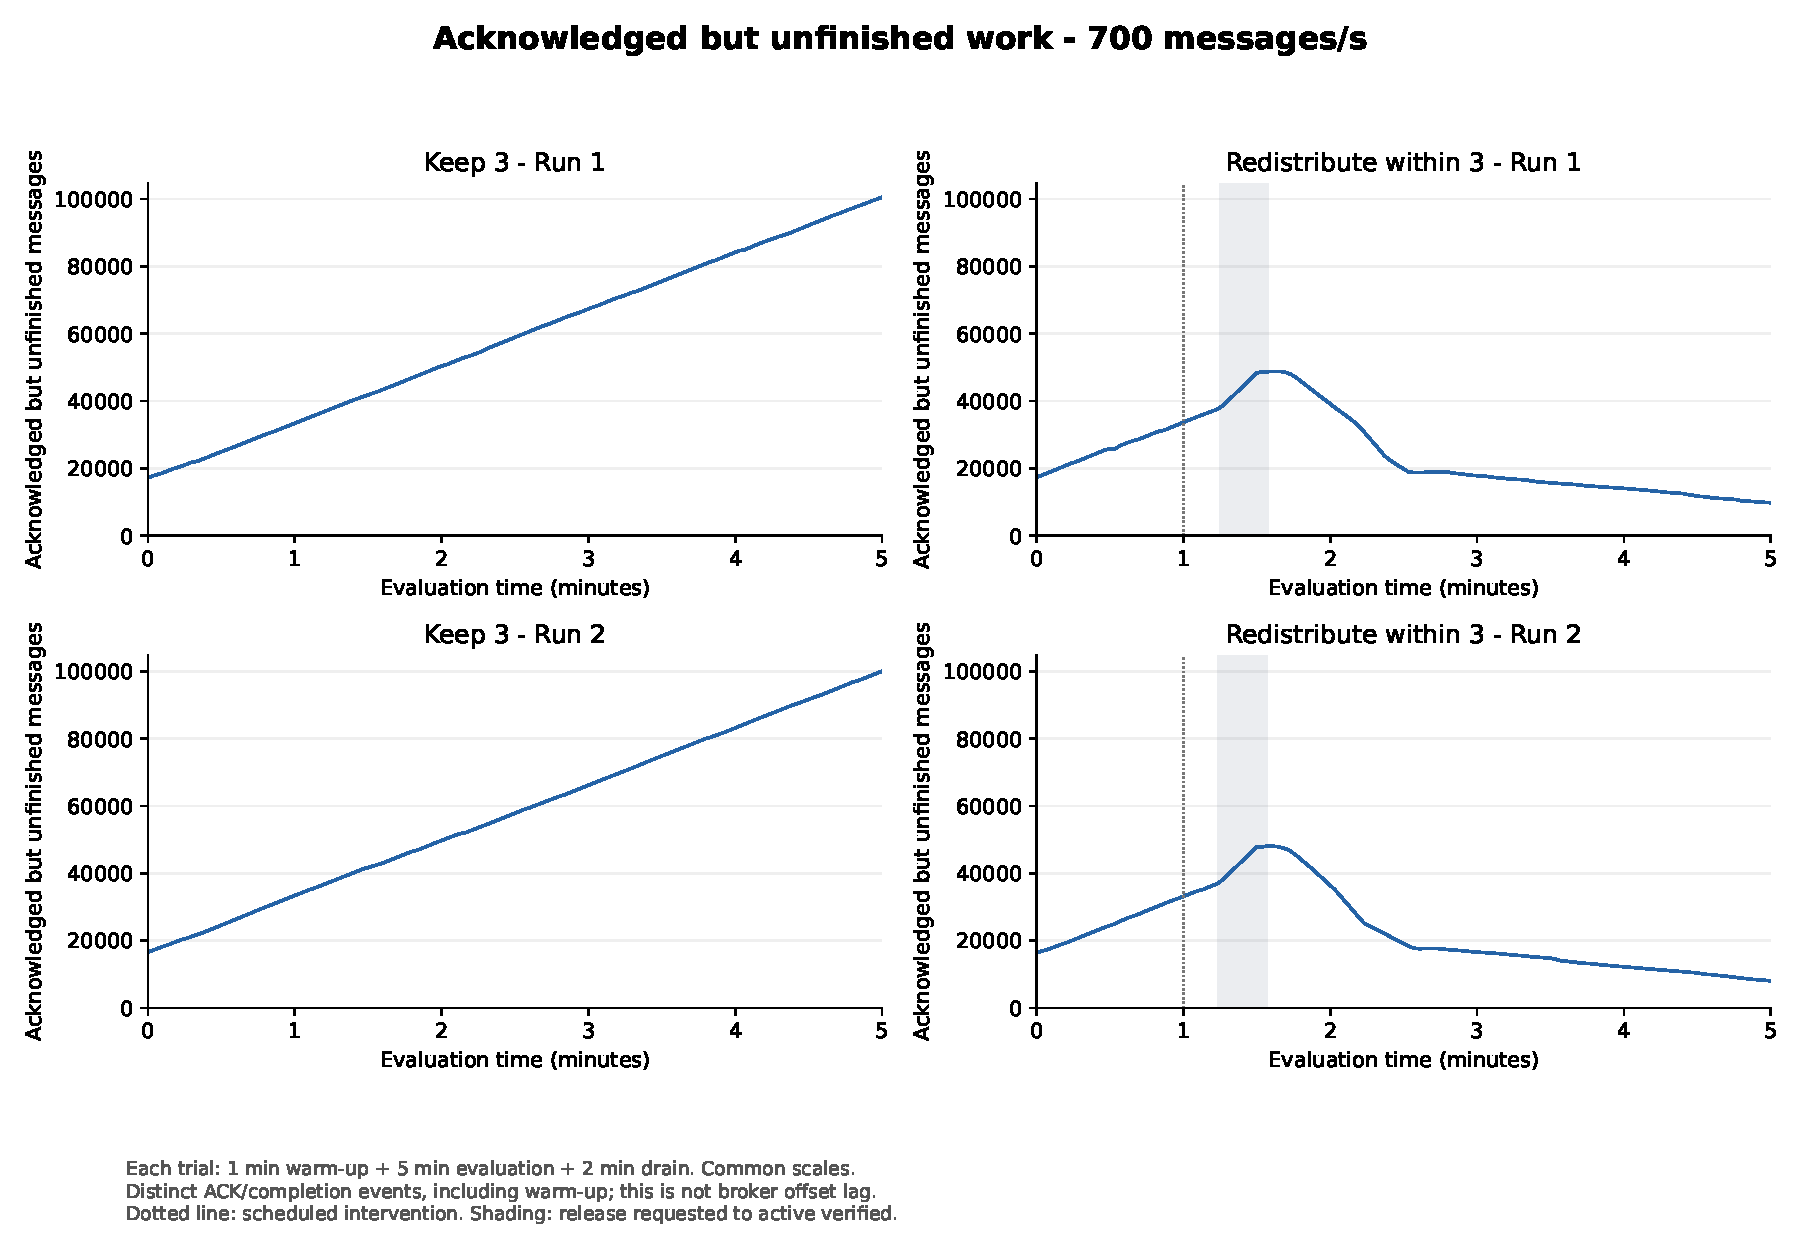
\includegraphics[width=\linewidth,height=5.1in,keepaspectratio]{figures/c2-redistribution-outstanding.pdf}
\caption{Distinct acknowledged messages not yet completed during the five-minute redistribution trials, including warm-up work. Event records show unfinished work decreasing after the intervention despite gaps in offset-based lag measurements. These curves are not the evaluation-only unfinished-message percentage at the drain cutoff.}
\label{fig:c2-redistribution-outstanding}
\end{figure}
\end{landscape}
\clearpage

% Ten-minute diagnostics are consolidated in the main results.
\endgroup

\subsection{Persistent-hot and partition-lag diagnostics}
These two earlier blocks each used a five-minute evaluation, one-minute warm-up and two-minute drain, with 210,000 successfully published evaluation messages per trial. Each block contains its own unchanged-assignment baseline and its intervention, each run twice. They remain separate comparisons rather than being pooled into the later ten-minute experiments. Tables~\ref{tab:live-performance}, \ref{tab:live-resources} and~\ref{tab:live-lag-coverage} collect the outcomes, resource use and lag summaries. The figures below add persistent-hot counts and maximum and mean partition lag.

The historical monitoring gaps are retained. Some predate the correction that initializes a returned-record position from a verified assignment offset while the client position remains unresolved. The correction was not applied retrospectively to invent missing values. Missing observations also restart the fifteen-observation persistence history, so the diagnostic gap may last longer than the ownership transfer itself. A shorter growth window cannot recover measurements that were never available. No comparison of these blocks with the later ten-minute blocks isolates duration alone: dates, selected partition identities and the monitoring implementation also changed.
The figures use the same measurement definitions as the proposal. These runs have five minutes of evaluation followed by two minutes of drain; warm-up is excluded from the resource totals. The one-second SLO calculation includes overdue unfinished messages.




\begin{figure}[!htbp]
\centering
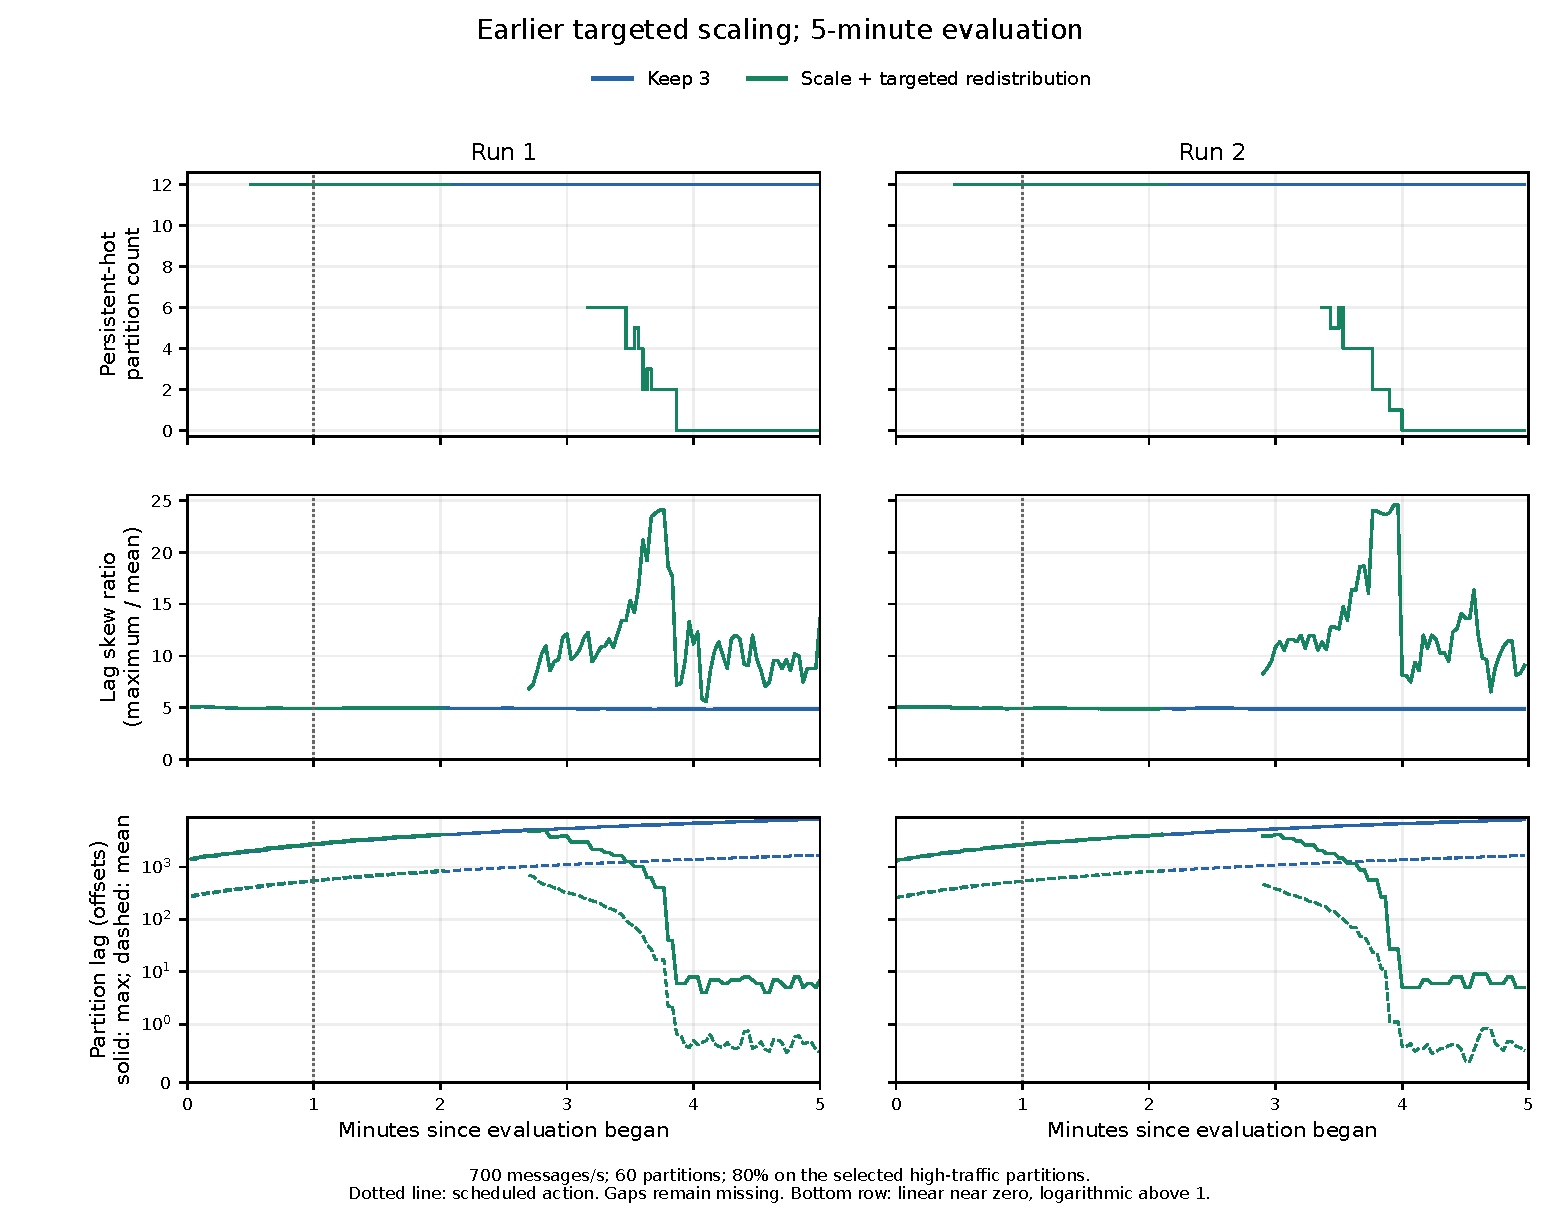
\includegraphics[width=\linewidth,height=.79\textheight,keepaspectratio]{figures/short-targeted-scaling-diagnostics.pdf}
\caption{Partition-level measurements during five-minute scaling-with-reassignment trials. The panels show persistent-hot-partition count, lag skew, and maximum and mean partition lag. Missing observations are left as gaps.}
\label{fig:short-targeted-scaling-diagnostics}
\end{figure}



\begin{figure}[!htbp]
\centering
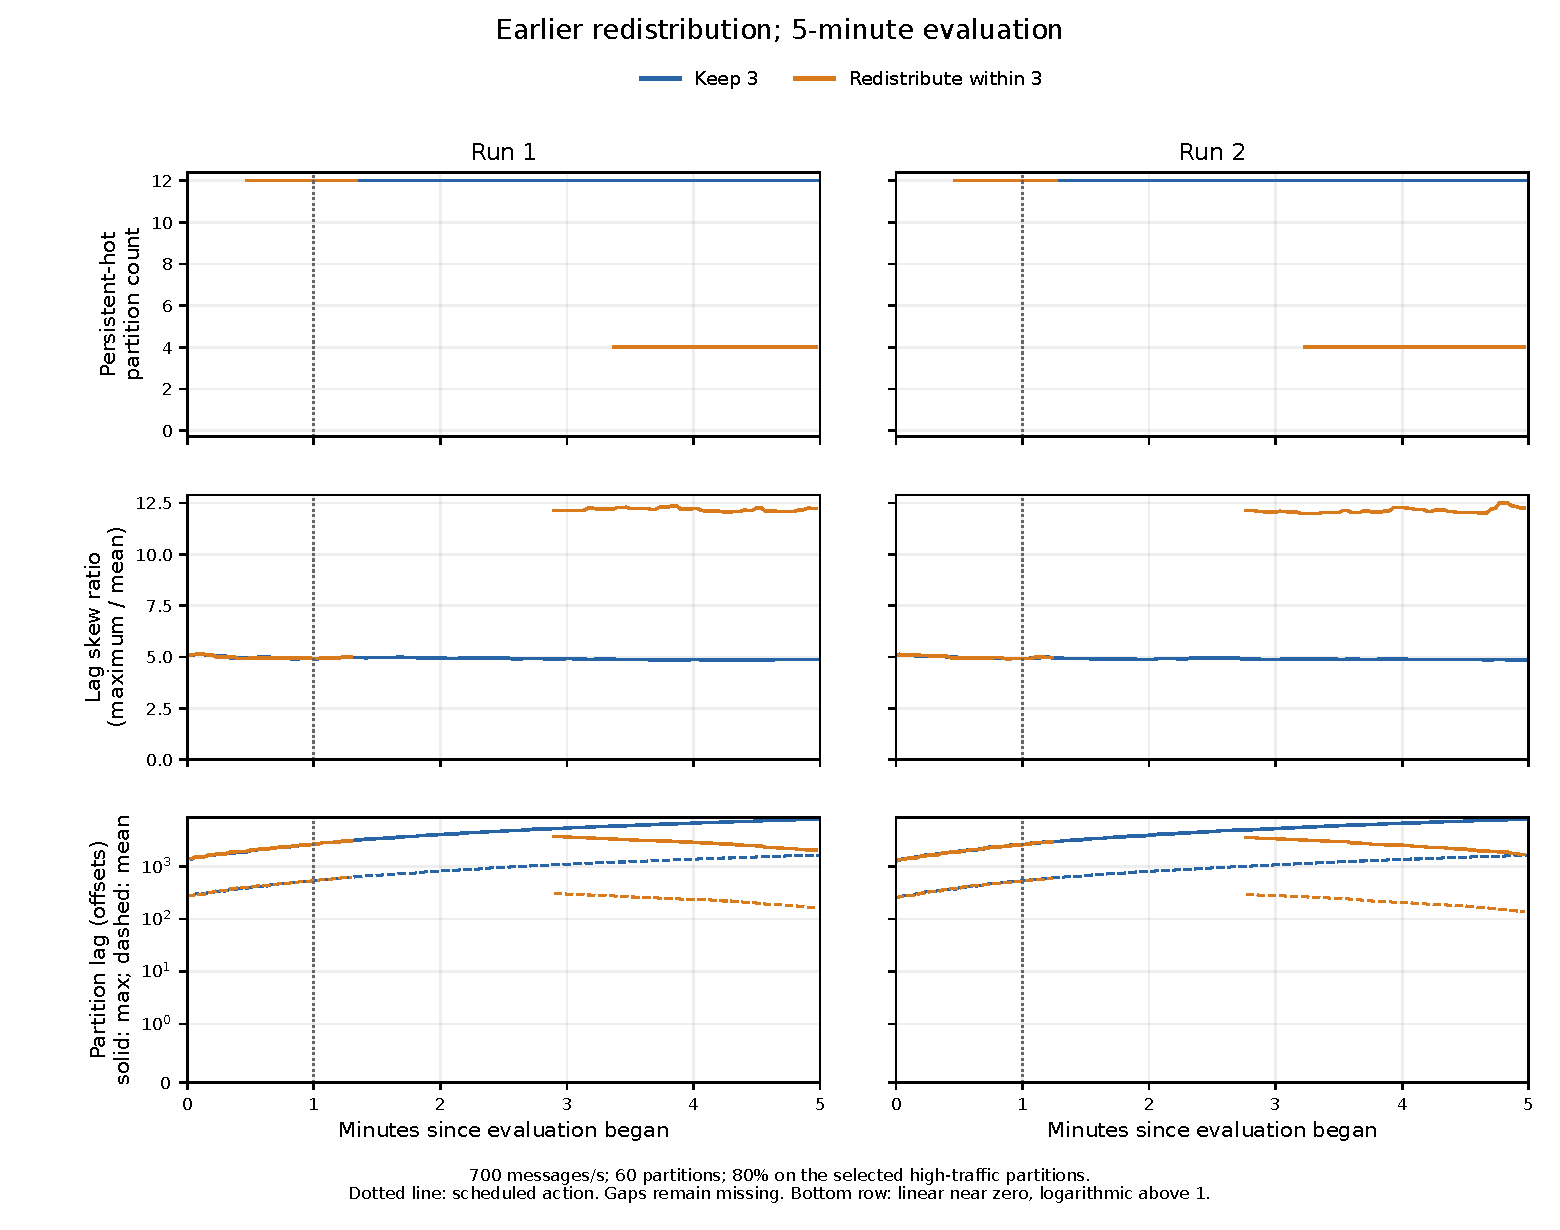
\includegraphics[width=\linewidth,height=.79\textheight,keepaspectratio]{figures/short-redistribution-diagnostics.pdf}
\caption{Partition-level measurements during five-minute reassignment trials with three consumers. The panels show persistent-hot-partition count, lag skew, and maximum and mean partition lag. Missing observations are left as gaps.}
\label{fig:short-redistribution-diagnostics}
\end{figure}
\clearpage

\clearpage
\section{Completion-Deadline Sensitivity}
\label{app:short-deadline-sensitivity}
The one-second SLO and half-second sensitivity threshold were applied retrospectively to these older trials. Overdue unfinished evaluation messages count as violations; no completion latency is assigned to them. The original 99-ms results remain in the experiment records.
\begin{table}[!htbp]
\centering\small
\setlength{\tabcolsep}{3pt}
\renewcommand{\arraystretch}{1.1}
\begin{tabular}{@{}lrrr@{}}
\toprule
Response & Run & Misses $>0.5$ s (\%) & Misses $>1$ s (\%)\\
\midrule
\multicolumn{4}{@{}l@{}}{\textbf{Scaling with targeted redistribution}}\\
Keep 3 & 1 & 83.447 & 83.418\\
Targeted scale 6 & 1 & 57.312 & 57.011\\
Keep 3 & 2 & 83.258 & 83.239\\
Targeted scale 6 & 2 & 58.572 & 58.171\\
\midrule
\multicolumn{4}{@{}l@{}}{\textbf{Redistribution within three consumers}}\\
Keep 3 & 1 & 83.438 & 83.413\\
Redistribute 3 & 1 & 61.794 & 61.591\\
Keep 3 & 2 & 83.278 & 83.241\\
Redistribute 3 & 2 & 61.100 & 60.840\\
\bottomrule
\end{tabular}
\caption{Completion-deadline sensitivity for the five-minute trials.}
\label{tab:short-targeted-scaling-deadline-sensitivity}
\label{tab:short-redistribution-deadline-sensitivity}
\end{table}

\begin{thebibliography}{1}
\bibitem{awsMskConsumerLag} Amazon Web Services. \emph{Monitor consumer lags}. Amazon MSK documentation. \url{https://docs.aws.amazon.com/msk/latest/developerguide/consumer-lag.html}. Accessed September 29, 2026.
\end{thebibliography}
\end{document}
